%----------------------------------------------------------------------------------------
%	PACKAGES AND OTHER DOCUMENT CONFIGURATIONS
%----------------------------------------------------------------------------------------

\documentclass[paper=letter, fontsize=11pt]{scrartcl} % A4 paper and 11pt font size

\usepackage[T1]{fontenc} % Use 8-bit encoding that has 256 glyphs
\usepackage{fourier} % Use the Adobe Utopia font for the document - comment this line to return to the LaTeX default
\usepackage[english]{babel} % English language/hyphenation
\usepackage{amsmath,amsfonts,amsthm} % Math packages
\usepackage{graphicx}
\usepackage{float}
\usepackage{import}
\usepackage{filecontents}
\usepackage{cite}
\usepackage{caption}
\usepackage{pdfpages}
\usepackage{booktabs}
\usepackage{dirtytalk}
\usepackage{url}
\usepackage{hyperref}
\usepackage{sectsty} % Allows customizing section commands
\allsectionsfont{\centering \normalfont\scshape} % Make all sections centered, the default font and small caps

\usepackage{fancyhdr} % Custom headers and footers
\pagestyle{fancyplain} % Makes all pages in the document conform to the custom headers and footers
\fancyhead{} % No page header - if you want one, create it in the same way as the footers below
\fancyfoot[L]{} % Empty left footer
\fancyfoot[C]{} % Empty center footer
\fancyfoot[R]{\thepage} % Page numbering for right footer
\renewcommand{\headrulewidth}{0pt} % Remove header underlines
\renewcommand{\footrulewidth}{0pt} % Remove footer underlines
\setlength{\headheight}{13.6pt} % Customize the height of the header

\numberwithin{equation}{section} % Number equations within sections (i.e. 1.1, 1.2, 2.1, 2.2 instead of 1, 2, 3, 4)
\numberwithin{figure}{section} % Number figures within sections (i.e. 1.1, 1.2, 2.1, 2.2 instead of 1, 2, 3, 4)
\numberwithin{table}{section} % Number tables within sections (i.e. 1.1, 1.2, 2.1, 2.2 instead of 1, 2, 3, 4)

% \setlength\parindent{0pt} % Removes all indentation from paragraphs - comment this line for an assignment with lots of text

\usepackage{rotating}

% Custom colors
\usepackage{color}
\usepackage{listings}
\usepackage{framed}
\usepackage{caption}
\usepackage{bm}
\usepackage{xfrac}
\captionsetup[lstlisting]{font={small,tt}}

\definecolor{mygreen}{rgb}{0,0.6,0}
\definecolor{mygray}{rgb}{0.5,0.5,0.5}
\definecolor{mymauve}{rgb}{0.58,0,0.82}

\lstset{ %
  backgroundcolor=\color{white},   % choose the background color; you must add \usepackage{color} or \usepackage{xcolor}
  basicstyle=\ttfamily\footnotesize, % the size of the fonts that are used for the code
  breakatwhitespace=false,         % sets if automatic breaks should only happen at whitespace
  breaklines=true,                 % sets automatic line breaking
  captionpos=b,                    % sets the caption-position to bottom
  commentstyle=\color{mygreen},    % comment style
  deletekeywords={...},            % if you want to delete keywords from the given language
  escapeinside={\%*}{*)},          % if you want to add LaTeX within your code
  extendedchars=true,              % lets you use non-ASCII characters; for 8-bits encodings only, does not work with UTF-8
  frame=single,                    % adds a frame around the code
  keepspaces=true,                 % keeps spaces in text, useful for keeping indentation of code (possibly needs columns=flexible)
  columns=flexible,
  keywordstyle=\color{blue},       % keyword style
  language=Python,                 % the language of the code
  morekeywords={*,...},            % if you want to add more keywords to the set
  numbers=left,                    % where to put the line-numbers; possible values are (none, left, right)
  numbersep=5pt,                   % how far the line-numbers are from the code
  numberstyle=\tiny\color{mygray}, % the style that is used for the line-numbers
  rulecolor=\color{black},         % if not set, the frame-color may be changed on line-breaks within not-black text (e.g. comments (green here))
  showspaces=false,                % show spaces everywhere adding particular underscores; it overrides 'showstringspaces'
  showstringspaces=false,          % underline spaces within strings only
  showtabs=false,                  % show tabs within strings adding particular underscores
  stepnumber=1,                    % the step between two line-numbers. If it's 1, each line will be numbered
  stringstyle=\color{mymauve},     % string literal style
  tabsize=4,                       % sets default tabsize to 2 spaces
}

\usepackage{enumitem}

% \usepackage{lineno}
% \linenumbers

%----------------------------------------------------------------------------------------
%	TITLE SECTION
%----------------------------------------------------------------------------------------

\newcommand{\horrule}[1]{\rule{\linewidth}{#1}} % Create horizontal rule command with 1 argument of height

\title{
\normalfont \normalsize
\textsc{University of California, Davis} \\ [25pt] % Your university, school and/or department name(s)
\horrule{2pt} \\[0.4cm] % Thin top horizontal rule
\huge Hubble Reboost Vehicle (HRV): \\ Preliminary Design Review % The assignment title
\horrule{2pt} \\[0.5cm] % Thick bottom horizontal rule
}

\author{
M. Cooper, H. Hasseeb, K. Jenks, J. Karasinski, \\M. LeVasseur, C. Lorenzen, J. Packer} % Your name

% \date{\normalsize\today} % Today's date or a custom date
\date{} % Today's date or a custom date

\begin{document}

\pagenumbering{gobble}
\maketitle % Print the title
\newpage

\pagenumbering{roman}

\tableofcontents
\newpage
% \listoffigures
% \newpage
% \listoftables
% \newpage

\pagenumbering{arabic}

%----------------------------------------------------------------------------------------
%	Introduction
%----------------------------------------------------------------------------------------

\section{Introduction}
% \begin{figure}[h!]
% \begin{center}
% 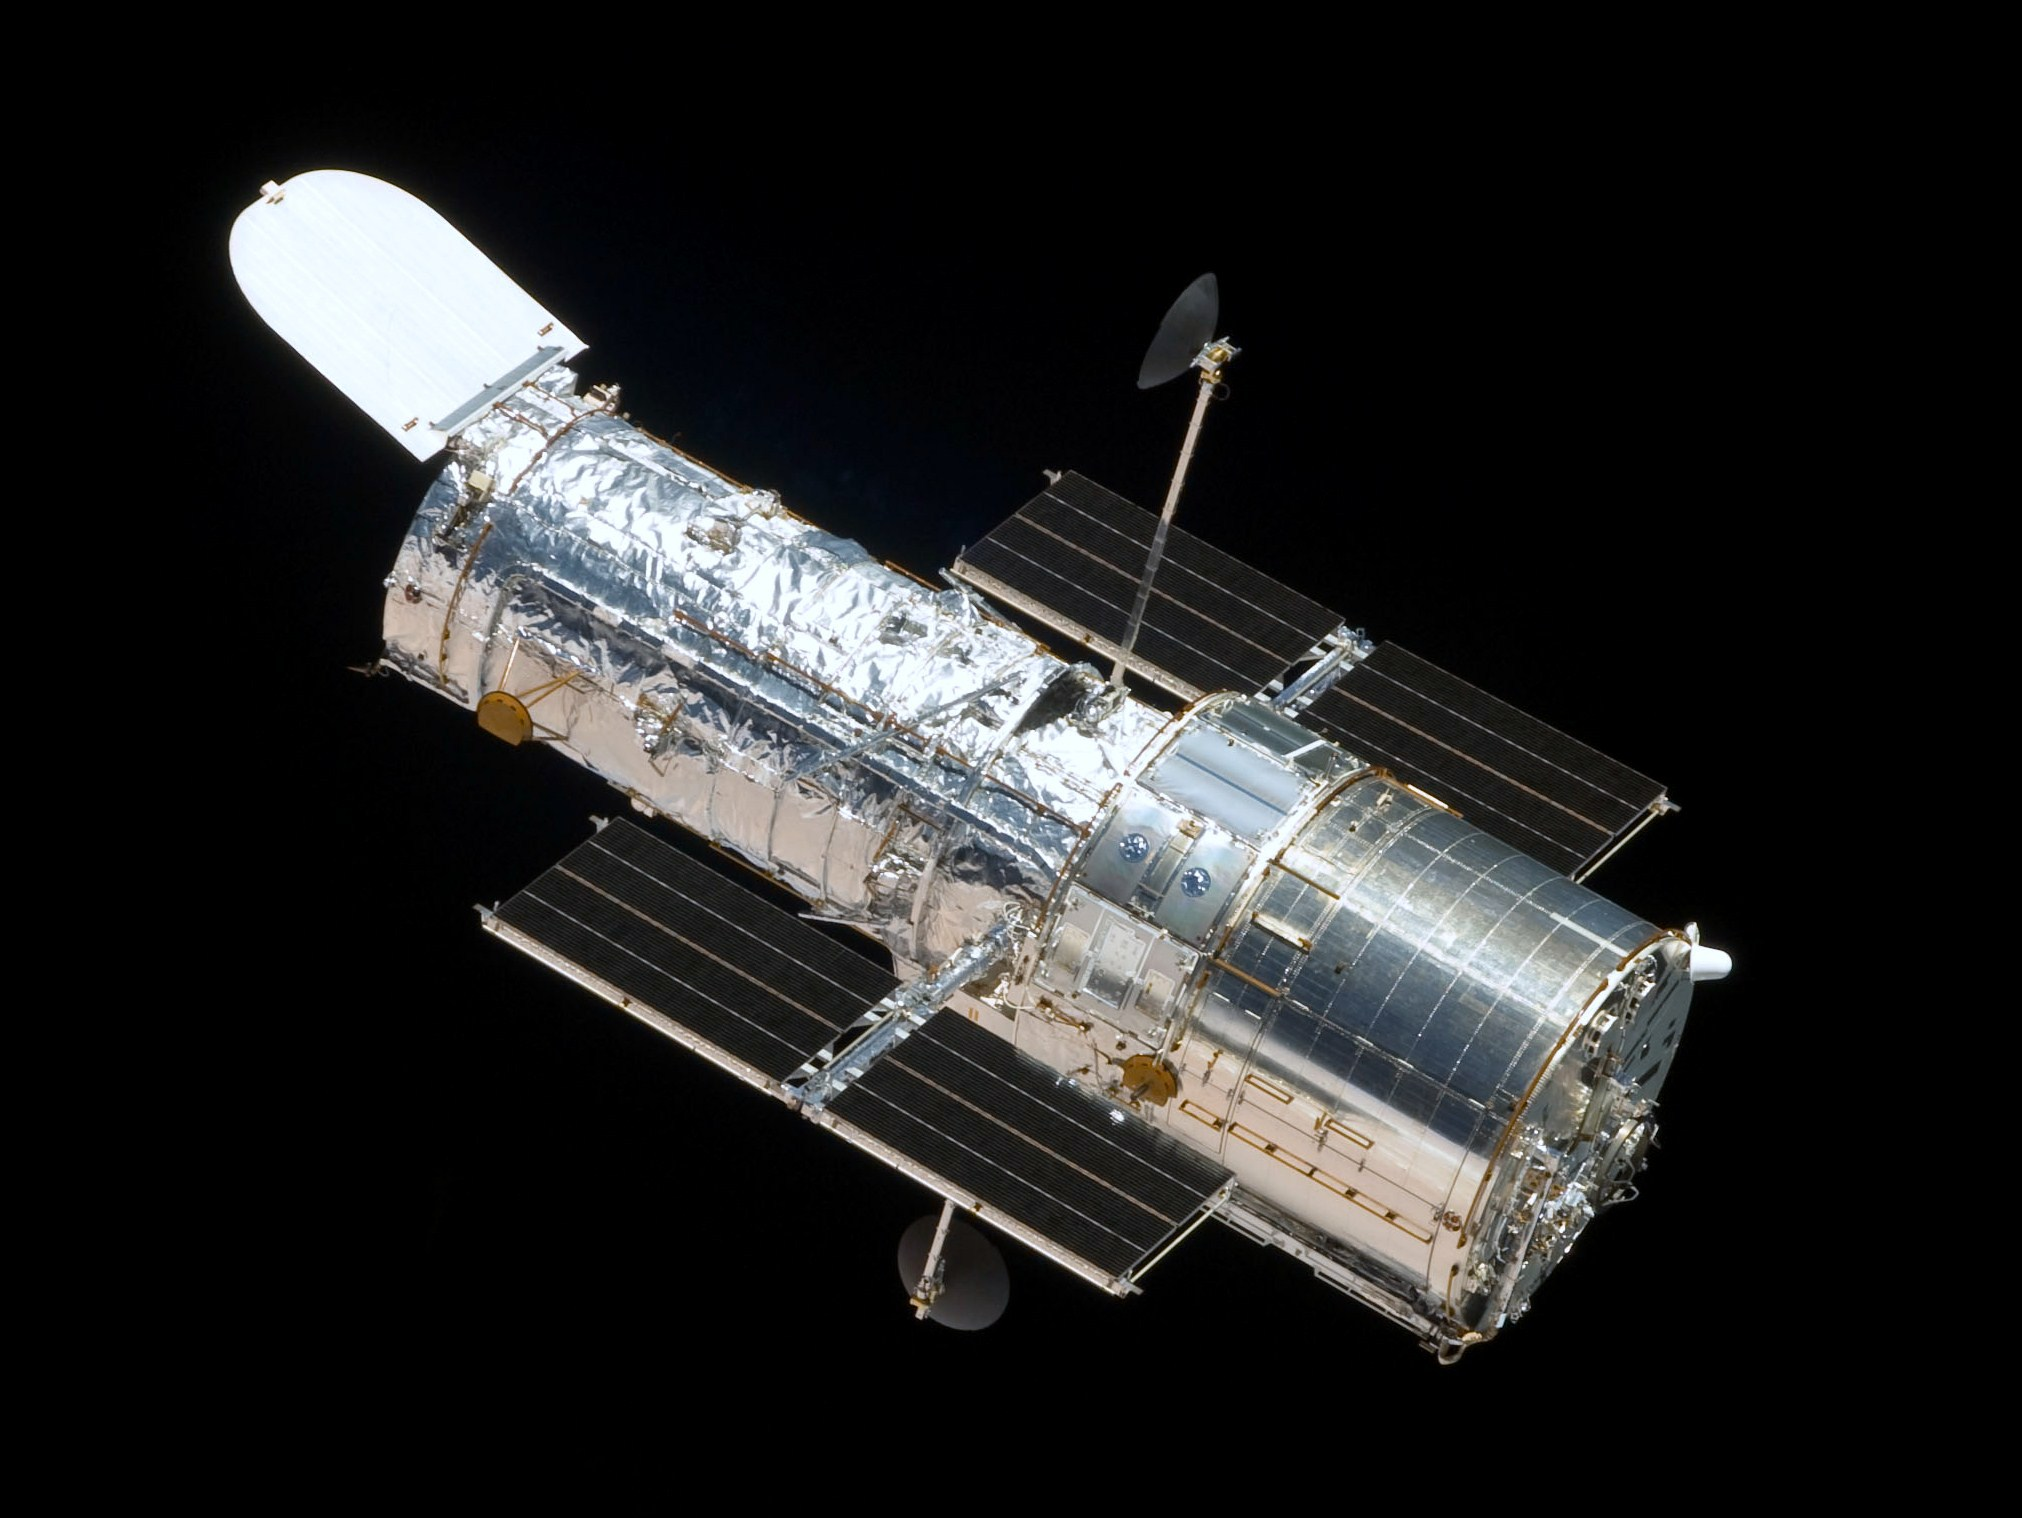
\includegraphics[width=1\textwidth]{imgs/HST-SM4.jpeg}
% \caption{The Hubble Space Telescope as seen from the departing Space Shuttle Atlantis, flying Servicing Mission 4 (STS-125), the fifth and final human spaceflight to it.}
% \label{fig:density}
% \end{center}
% \end{figure}

\begin{figure}[tbh]
\begin{center}
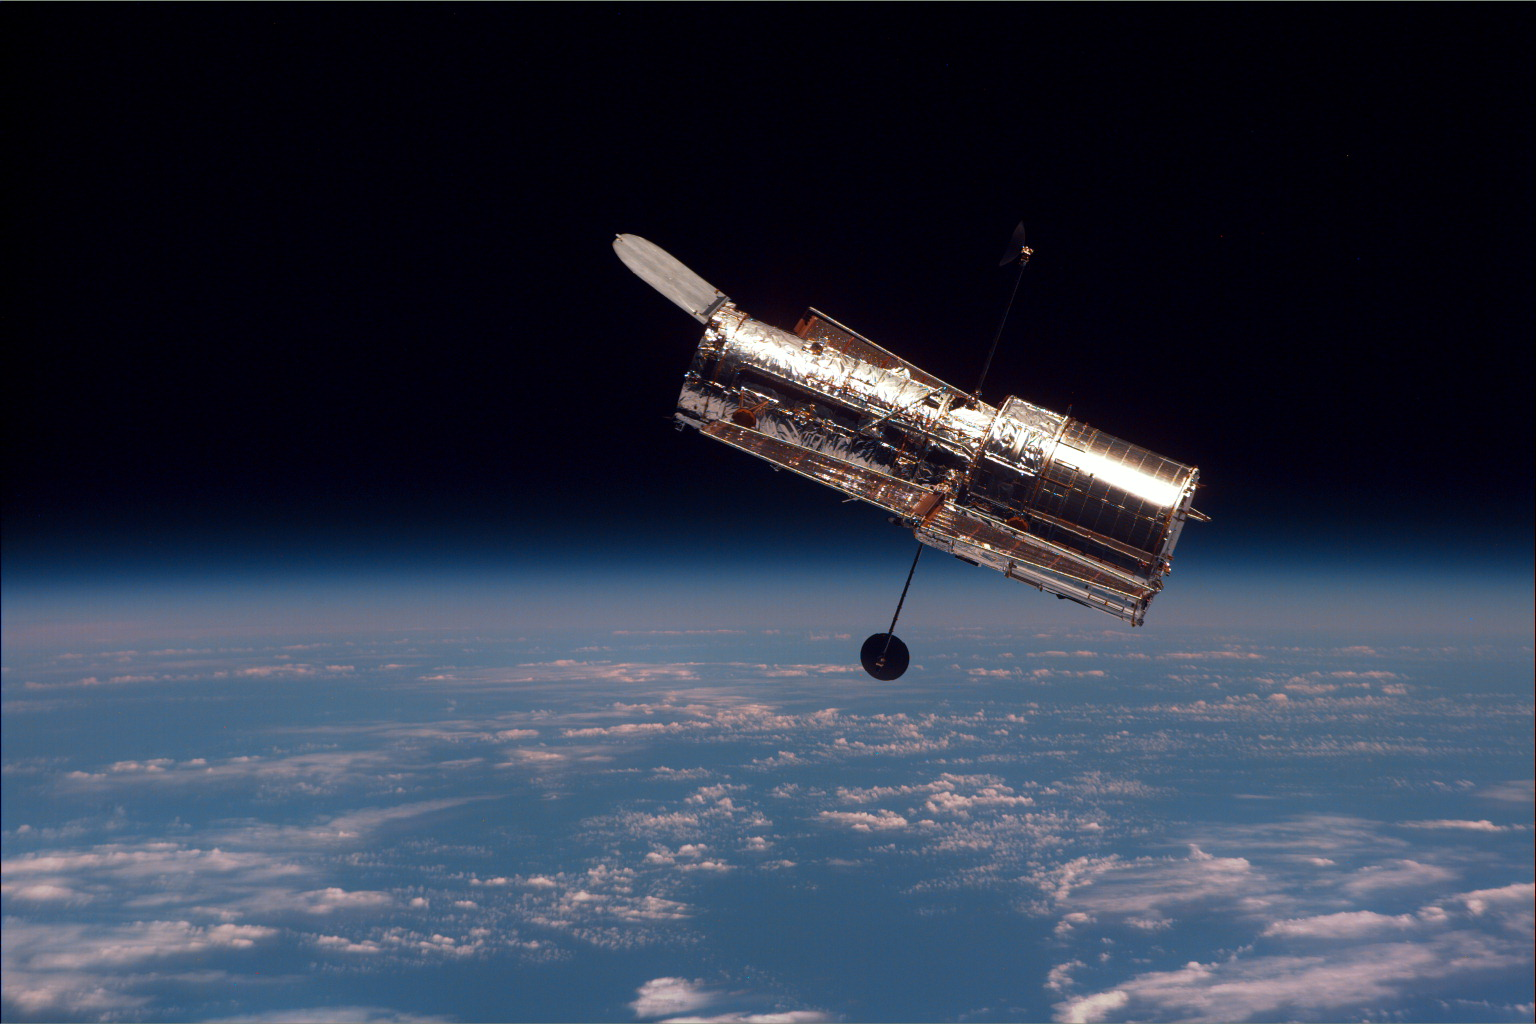
\includegraphics[width=1\textwidth]{imgs/hst.jpg}
\caption{This photograph of NASA's Hubble Space Telescope was taken on the second servicing mission to the observatory in 1997.}
% \label{fig:density}
\end{center}
\end{figure}

\subsection{Importance of Mission}
On April 24, 1990, the Hubble Space Telescope (HST) was launched on the space shuttle Discovery from Kennedy Space Center in Florida. Since its launch, it has traveled more than 3 billion miles along the circular low Earth orbit, and has made more than 1.2 million scientific observations. The reboost mission will play a crucial role in extending the HST lifespan, and allow it to make more scientific observations.

\par The HST had been developed to gather light from cosmic objects to understand our universe. The necessity for this telescope was the insufficient image resolution of the pre-existing ground-based telescopes resulting from the interference with the earth's atmosphere. The HST was able to provide stable imagery with a sensitivity to wavelengths ranging from ultraviolet to near infrared, which were inaccessible to ground-based telescopes.

\par Major scientific discoveries have risen from the HST mission. Based on its observations, the rate at which the universe is expanding had been determined, the age of the universe had become more refined, and distances to Cepheid variable stars had been computed to an accuracy of 10\%. In addition, HST has discovered galaxies billions of light years away, distant supernovae, and evidence of black holes. More than 9,000 technical papers have been published on astronomical observations made by the HST. In sum, the reboost mission can extend the HST lifespan and lead to key future breakthroughs in our understanding of the universe.

\subsection{Mission Purpose}
The Hubble Reboost Vehicle (HRV) shall extend the Hubble Space Telescope's (HST) operational lifetime to 5 years beyond the James Webb Space Telescope's (JWST) October 2023 launch date. This will be achieved by reboosting HST into a circular orbit such that its useful operation until orbit decay is extended to October of 2028.

\subsection{Mission Timeline}
The mission to reboost the HST will be composed of multiple phases, as described in the table below. The entire duration of the mission will be no longer than 60 hours.

A launch date (September 2019) was chosen to provide the most direct route to the HST. By launching when the HST is directly over the launch site (Kennedy Space Center), the reboost vehicle will match its inclination and longitude of ascending node. This prevents the need for any costly plane changes.


\begin{table}[H]
\begin{center}
\begin{tabular}{l r}
\toprule
Mission Phase & Duration (hours) \\
\midrule
1. Launch (delivered to parking orbit) & 1.27 \\
2. Maintain parking orbit for necessary phasing time & up to 24 \\
3. Transfer to HST altitude & 1.53 \\
4. Rendezvous and dock with the HST & 0.75 \\
5. Boost HST to new orbit & 1.60 \\
6. Undock and separate from HST & 1.5 \\
7. Maintain orbit for necessary phasing time & up to 24 \\
8. Deorbit to burn up in the atmosphere & 0.77 \\
\bottomrule
Max time: & 55.22 \\
\bottomrule
\end{tabular}
\end{center}
% \caption{}
% \label{properties}
\end{table}

\subsection{Stakeholders}

% \begin{figure}[H]
%     \centering
%     \begin{subfigure}[b]{0.4\textwidth}
%         \includegraphics[width=\textwidth]{imgs/xtreme_deep_field.png}
%     \end{subfigure}
%     ~ %add desired spacing between images, e. g. ~, \quad, \qquad, \hfill etc.
%     %(or a blank line to force the subfigure onto a new line)
%      \begin{subfigure}[b]{0.4\textwidth}
%         \includegraphics[width=\textwidth]{imgs/Pillars_of_creation_2014_HST_WFC3_medium_res.jpg}
%     \end{subfigure}
%     ~ %add desired spacing between images, e. g. ~, \quad, \qquad, \hfill etc.
%       %(or a blank line to force the subfigure onto a new line)
%     \begin{subfigure}[b]{0.4\textwidth}
%         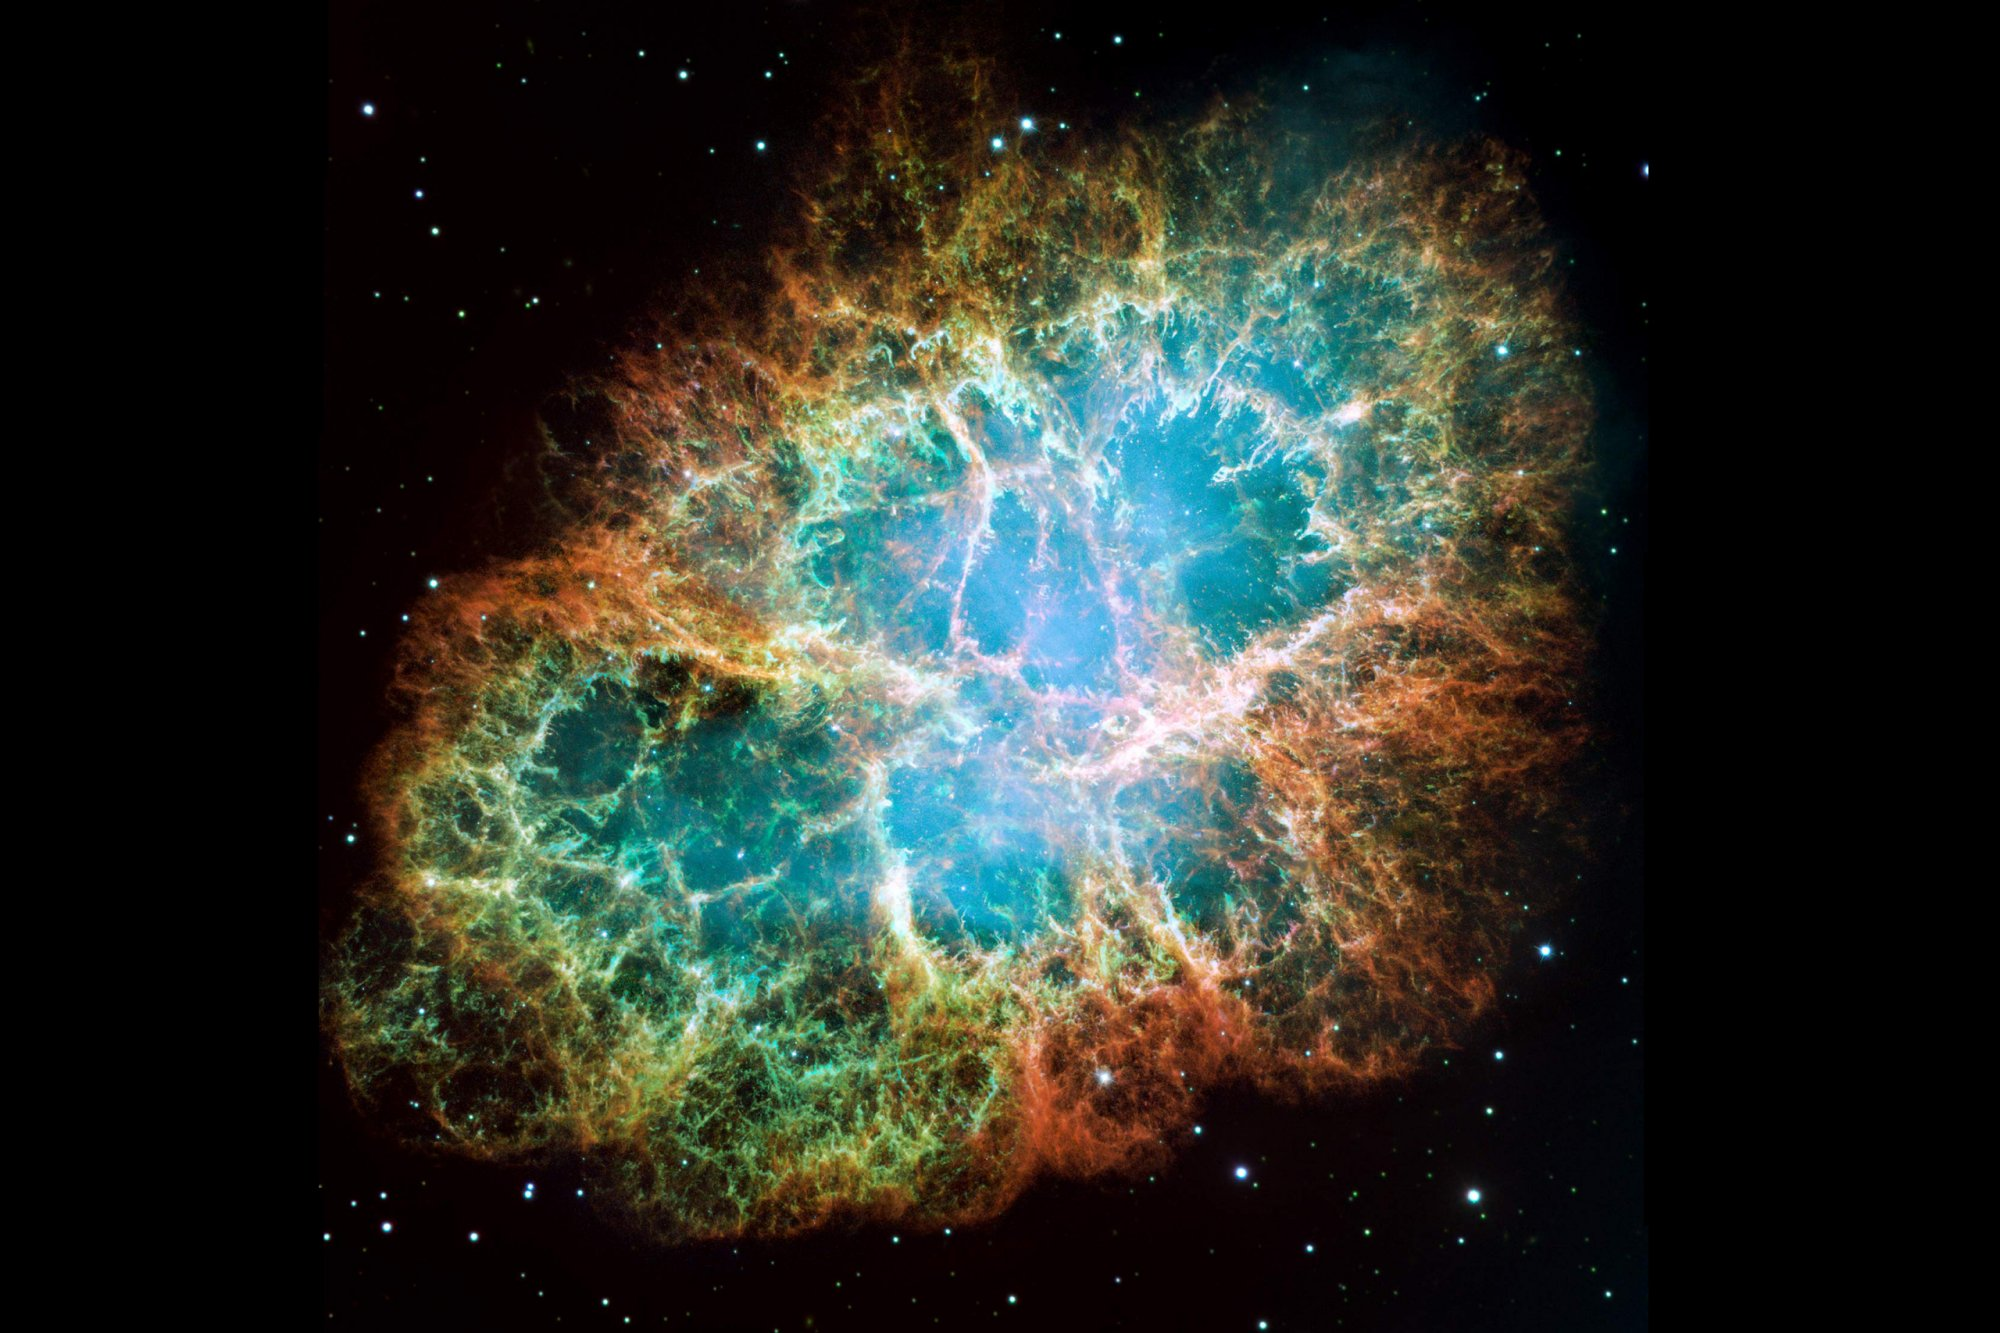
\includegraphics[width=\textwidth]{imgs/crab.jpg}
%     \end{subfigure}
%     ~ %add desired spacing between images, e. g. ~, \quad, \qquad, \hfill etc.
%     %(or a blank line to force the subfigure onto a new line)
%     \begin{subfigure}[b]{0.4\textwidth}
%         \includegraphics[width=\textwidth]{imgs/M104_ngc4594_sombrero_galaxy_hi-res.jpg}
%     \end{subfigure}
%     \caption{Hubble has taken many photos of iconic space objects, including the Hubble Extreme Deep Field, Pillars of Creation, the Crab Nebulae, and the Sombrero Galaxy.}
%     \label{fig:animals}
% \end{figure}

Hubble has a many stakeholders. Hubble has made a large number of important discoveries, leading to significant changes in how we think about the universe. Among its primary mission targets was to measure distances to Cepheid variable stars more accurately than ever before. Accurate measurement of the Cepheid variable constrains the value of the Hubble constant, the measure of the rate at which the universe is expanding, which has allowed scientists to very accurately calculate the age of the universe.

Hubble has also been extremely successful in generating public relations, both due to its scientific achievements and the wealth of memorable images it has produced. The public is extremely invested in Hubble, both from their large contributions to its construction and operational costs. Aside from Hubble's scientific goals, it also helps fulfill two of NASA's key agency objectives to
\begin{itemize}
\setlength\itemsep{0em}
\item Improve science literacy by engaging the public in NASA missions and discoveries, and their benefits, through such avenues as public programming, community outreach, mass media, and the Internet.
\item Increase public awareness and understanding of how research and innovations in aerospace technology affect and improve the quality of life.
\end{itemize}

The HST was built by the United States space agency NASA, with contributions from the European Space Agency (ESA). The Space Telescope Science Institute (STScI) selects Hubble's targets and processes the resulting data, while the Goddard Space Flight Center controls the spacecraft~\cite{hubble_essentials}. As such, NASA, ESA, STScI, and NASA Goddard are among the chief stakeholders in a robotic reboost mission. Other organizations that have constructed and worked with HST, such as JPL and ITT, would obviously be affected by our interacting with HST. A list of the most important stakeholders contains
\begin{itemize}
\setlength\itemsep{0em}
\item NASA Headquarters (HQ)
\item NASA Goddard Space Flight Center (GSFC)
\item The European Space Agency (ESA)
\item The Space Telescope Science Institute (STScI)
\item The Jet Propulsion Laboratory (JPL)
\item ITT (formerly Kodak)
\item International universities and space agencies
\item The National Reconnaissance Office (NRO)
\item Department of Defense (DoD)
\item Other governmental organizations
\item The public
\end{itemize}

While none of the stakeholders involved in the Hubble project would object to extending the project for several years, damaging Hubble would be much worse than leaving it in it's current orbit. As such, the primary goal of the HRV is to do no harm to Hubble. The mission can succeed only if we can it can be accomplished within the stakeholders' limits of acceptable risk.

\subsection{Concept of Operations}
\begin{figure}[H]
\begin{center}
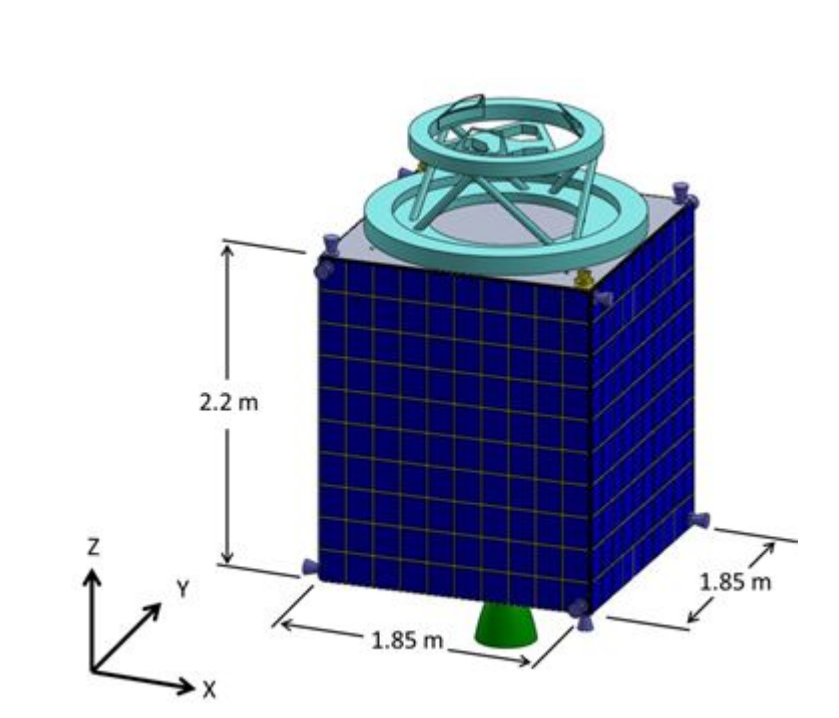
\includegraphics[width=.75\textwidth]{spacecraft_final.png}
\caption{Hubble Reboost Vehicle.}
% \label{fig:density}
\end{center}
\end{figure}

HRV mission control will be performed from NASA's Goddard Space Flight Center (GSFC). The site was chosen in order to incorporate several members of the HST team into the HRV team. Communication to both the HRV and HST will be performed primarily through the White Sands Complex and existing Tracking and Data Relay Satellite System (TDRSS). NASA's Kennedy Space Center (KSC) was selected as the launch site in order to launch into HST's orbit.

Upon launch the craft will be under the control of the United Launch Alliance (ULA). Telemetry will be monitored by the GSFC ground crew but control will not be handed over until the payload fairing separation. Upon being ejected from the payload, any primary systems not running start up. The HRV ``wakes up'' and starts to determine its attitude and position. During this time GSFC is also making attempts for their first radio acquisition. With the system fully booted and telemetry coming in, the HRV can start its mission.

The first step of the mission is to increase the HRV orbit out of the parking orbit. This requires a large burn to transfer to an orbit closer to HST then another burn to circularize. Any mission critical operation such as this requires confirmation from the ground crew. HRV telemetry and the calculated burn are relayed to the ground crew. The ground crew confirms the information and gives the HRV the go ahead to perform the burn. Any time the HRV is waiting for a critical response, a timer is also started. If an extended period of time passes without a command then end-of-mission deorbit procedures are started.

After circularizing to an orbit below HST, the rendezvous starts. The HRV is allowed to phase towards the HST until starting the final approach. The final approach is performed in two stages depending on the distance from the target. At this point the HST starts relaying telemetry directly to HRV through the low-gain antennas. In the last moments of docking the craft is given more autonomy. There is no time to check every correction; therefore a standard manual abort/override is built into the system.

Once the berthing has taken place, the HST's attitude control system is used to repoint the pair of craft for a prograde burn. HRV performs the burn to increase the craft's orbit. HST rotates the pair of craft for a retrograde burn. HRV performs a burn to circularize into the final target orbit. All of these are critical operations requiring the ground crew to confirm any actions.

With the main goal of the mission done, HRV detaches and separates to a safe distance. Once a sufficient distance is achieved from HST a final large burn is performed to deorbit the HRV. Before this burn is performed the final entry point is recalculated to ensure entry over the Pacific Ocean.


%----------------------------------------------------------------------------------------
%	REQUIREMENTS
%----------------------------------------------------------------------------------------

\section{Requirements} \label{section:reqs}

\subsection{Customer Requirements}

The mission of the Hubble Reboost Vehicle (HRV) is to
\say{Reboost HST spacecraft to circular orbit so that useful operation until orbit decay is extended to 5 years beyond the JWST 10/23 launch date, i.e. to 10/28.} \\
\\
Thirteen requirements of the vehicle are taken directly from the Mission Requirements. To this end, the HRV must
\begin{enumerate}[label=(\alph*)]
\item Launch on an existing US launcher from Cape Canaveral into the HST orbit
\item Rendezvous and dock with HST
\item Use HST or rebooster ADCS to orient combined spacecraft for reboost
\item Reboost thrust must result in solar array boom deflection of no more than 50 cm
\item Undock from HST and destructively deorbit into atmosphere
\item Send and receive state-vector, attitude, and system health telemetry to/from HST
\item Send and receive state-vector, attitude, and system health telemetry to/from NASA Mission Control Center (MCC), either directly, or indirectly via HST and or TDRS satellites
\item Be able to recover from one Single Event Upset per hour in the onboard Command and Control Computer
\item No requirement on duration of mission
\item Power and thermal requirements not specified --- to be determined by design to meet mission objectives
\item Main body of spacecraft bus must include MMOD shielding
\item ADCS must be able to recover from/override both jet-fail-on, and jet-fail cases during proximity operations without collision of mission failure
\item Loss of communications between rebooster and HST or MCC must not result in collision
\end{enumerate}

\subsection{Technical Requirements}

From the customer requirements come the technical requirements.  The technical requirements break the customer requirement up into specific goals to be accomplished by the summation of subsystems within the HRV.

\begin{enumerate}
\item The HRV shall not damage the HST (Primary Mission)
\item The HRV shall reboost HST to an altitude that extends HST's operational timeline to October 2028 (Primary Mission)
\item The HRV shall be within the mass/volume limits of an available launch vehicles (a)
\item The HRV shall have the ability to perform proximity operations with HST (b)
\item The HRV shall have the ability to dock and undock with HST (b,e)
\item The HRV or HST shall have the ability to adjust the attitude of the combined HST and HRV (c)
\item The HRV shall limit acceleration of HST such that the solar array boom deflection is no more than 50 cm (d)
\item The HRV shall have sufficient delta-V remaining to destructively deorbit at the end of the mission (e)
\item The HRV shall have the ability to determine its state vector (f)
\item The HRV shall have the ability to determine its attitude (f)
\item The HRV shall have the ability to determine its system health (f)
\item The HRV shall have the ability to transmit and receive data to HST (f)
\item The HRV shall have the ability to transmits and receive data with ground control (g)
\item The HRV shall have multiple rad tolerant processors. (h)
\item The HRV shall perform its mission until complete or the mission has been aborted (i)
\item The HRV shall store sufficient power (j)
\item The HRV shall generate sufficient power. (j)
\item The HRV shall have the ability to stay within acceptable thermal ranges. (j)
\item The HRV shall have sufficient MMOD shielding to minimize risk due to impact (k)
\item The HRV shall be able to recover from thruster failure (l)
\item The HRV shall have a failsafe to safely deorbit in case of communication loss. (m)
\end{enumerate}

\subsection{System Requirements}
The technical requirements are then distributed among the relevant subsystems to make system requirements to be fulfilled by the various components.

\subsubsection{Electronics/Power}
\begin{enumerate}
\item The C\&DH computer shall utilize a minimum of three processors (h)
\item The C\&DH shall utilize a failsafe program to deorbit the HRV in case of communication loss (m)
\item The solar panels shall generate sufficient energy (j)
\item The primary battery cells shall store enough power to maintain operation standard operation (j)
\item The primary battery cells shall store enough power for the entire rendezvous phase
\item The backup battery cells shall store enough power for the entire rendezvous phase
\end{enumerate}

\subsubsection{Communications}
\begin{enumerate}
\item The communication system shall utilize an S-band antenna (f)
\item The communication system shall utilize a Ku-band antenna (g)
\end{enumerate}

\subsubsection{Guidance, Navigation, and Control}
\begin{enumerate}
\item The ADCS shall detect the attitude of the HRV. (f)
\item The ADCS shall determine the absolute and HST-relative state vectors. (f)
\item The ADCS shall process complex types of data and transfer attitude data to the ground station. (g)
\item The ADCS shall provide required control torques to adjust attitude and stabilize the HRV.(b)
\item The ADCS shall be able to recover from/override both jet-fail-on, and jet-fail cases. (l)
\end{enumerate}


\subsubsection{Rendezvous and Docking}
There is one customer requirement to consider in designing the rendezvous and docking. \say{(b), Rendezvous and dock with HST}.

To address this customer requirement, several system level requirements are set
\begin{enumerate}
\item A rendezvous plan shall be established.
\item A docking plan shall be established.
\item The rendezvous and docking plan shall have sufficient flight heritage.
\item Sufficient sensors shall exist to measure the state of the HRV for both absolute and relative navigation during rendezvous and docking.
\item Sufficient knowledge and control over the vehicle state shall be present in order to meet soft capture mechanism (SCM) docking requirements.
\end{enumerate}


\subsubsection{Propulsion}
The propulsion requirements for the mission depend on the maneuvering required for each phase. The propulsion requirements for each phase of the mission can be summarized as follows

\begin{enumerate}
\item Launch
\begin{enumerate}
    \item The propellant tanks shall carry enough propellant to make up for orbital insertion inaccuracy (-30 km) (a)
    \item $\Delta V$ included in phase 3 (a)
\end{enumerate}
\item Parking Orbit
\begin{enumerate}
    \item The parking orbit shall be maintained for the phasing time required. (b)
    \item The propellant tanks shall carry enough propellant to overcome perturbations \& dodge debris while in the parking orbit (b)
    \item The propulsion system shall provide a total $\Delta V$ of approximately 150 m/s for this segment of the mission (b)
\end{enumerate}
\item Transfer to HST
\begin{enumerate}
    \item The propulsion system shall enable the HRV to perform a Hohmann transfer (two burns) to the HST altitude (b)
    \item The propulsion system shall provide a total $\Delta V$ of approximately 207 m/s (b)
\end{enumerate}
\item Rendezvous and Dock
\begin{enumerate}
    \item The propulsion system shall utilize cold gas thrusters for propulsion during rendezvous and dock to avoid damage or contamination to HST (b)
    \item The propulsion system shall provide a total $\Delta V$ of approximately 50 m/s for this segment of the mission (b)
\end{enumerate}
\item Reboost
\begin{enumerate}
    \item The propulsion system shall enable the HRV to perform a Hohmann transfer (two burns) with the HST attached (Primary Mission)
    \item The re-boost acceleration provided by the propulsion system shall not damage the HST (d)
    \item The propulsion system shall provide a total $\Delta V$ of approximately 46 m/s for this segment of the mission (Primary Mission)
\end{enumerate}
\item Undock and Separation
\begin{enumerate}
	\item The docking mechanism shall contain a spring to facilitate separation (e)
    \item The propulsion system shall utilize cold gas thrusters to avoid damage or contamination to the HST (e)
    \item The $\Delta V$ required for undock and separation is negligible
\end{enumerate}
\item Maintain Orbit for Phasing Time
\begin{enumerate}
    \item The orbit shall be maintained for the phasing time required to separate to a safe distance from HST (e)
    \item The propellant tanks shall carry enough propellant to overcome perturbations while waiting for the deorbit window (e)
    \item The $\Delta V$ required for maintenance of the reboosted orbit is negligible.
\end{enumerate}
\item Deorbit
\begin{enumerate}
    \item The propulsion system shall perform a burn to deorbit the HRV to the upper atmosphere (120 km) over the ocean (e)
    \item The propulsion system shall provide a total $\Delta V$ of approximately 140 m/s for this segment of the mission (e)
\end{enumerate}
\end{enumerate}


\subsubsection{MMOD Shielding}
\begin{enumerate}
\item The MMOD shielding shall be able to withstand orbital debris given a 99.99\% probability of no penetration, based on a probabilistic orbital debris model (k)
\item The MMOD shielding shall be applicable over the entire mission in all orbits (k)
\end{enumerate}


\subsubsection{Structure}
\begin{enumerate}
\item Primary
\begin{enumerate}
\item The docking platform shall interface with HST soft capture mechanism (b)
\item The mating parameters shall remain within limits that ensure structural health (b)
\item The HST solar arrays shall be oriented for minimal deflection during reboost(d)
\item The docking platform shall reliably un-mate from SCM with redundant mechanical system (e)
\end{enumerate}
\item Launch
\begin{enumerate}
\item The structure shall meet factor of safety mechanical stress requirements for maximum expected quasi-static longitudinal and lateral accelerations sustained during launch (a)
\item The structure shall meet factor of safety mechanical stress requirements for vibration and shock loads sustained during launch (a)
\item The structure shall have first modes of natural frequency in thrust and lateral directions above the values sustained during launch (a)
\end{enumerate}
\item Dimensional
\begin{enumerate}
\item The structural volume shall be sufficient to contain all mission critical hardware (Mission Primary)
\item The structural dimensions shall be chosen to
\begin{enumerate}
\item Contain adequately sized propellant tanks (Mission Primary)
\item Properly interface with SCM on HST (e)
\item Properly interface with launch vehicle (a)
\item Fit within launch vehicle fairing (a)
\end{enumerate}
\end{enumerate}
\end{enumerate}

\subsubsection{Thermal}
\begin{enumerate}
\item The thermal radiators shall expel sufficient heat to prevent overheating (j)
\end{enumerate}


%----------------------------------------------------------------------------------------
%	FMEA
%----------------------------------------------------------------------------------------

\section{Failure Mode and Effects Analysis}
In order to better understand the inherent risks associated with the mission, a failure mode and effects analysis was made. The purpose was to systematically list out all of the potential failure modes and their effects that could be encountered during the mission, and establish counteractive measures to mitigate the risks. The FMEA used for the HRV analysis is an adapted model from a military specification~\cite{MIL-STD-1629A} and SMAD~\cite{ref12_8}.

\subsection{FMEA Breakdown}
Each row in the FMEA table (see Appendix~\ref{App:FMEA}) represents a potential hazard that the spacecraft might encounter on its mission. Hazards can range from the launch vehicle vibrating the spacecraft to the battery not being able to hold enough charge to power the spacecraft electronics. Each failure mode has a severity classification and an occurrence level that relate to the danger the failure could cause to the mission and the probability that it will happen, respectively. These two items are then combined to calculate a risk for that failure mode.

\subsubsection{Severity Classification}
Severity classifications are assigned to provide a qualitative measure of the worst potential consequences resulting from a design error or item failure. Table~\ref{table:severity} translates the qualitative impact of a failure mode into a quantitative score that can be later used in the FMEA.

\begin{table}[H]
\begin{centering}
\begin{tabular}{l c l}
	\toprule
	Severity Classification & Score & Description \\
	\midrule
	Category I              & 5     & \begin{tabular}{@{}l@{}}\textbf{Catastrophic} - A failure that may cause spacecraft \\ obliteration, or significant damage to another \\ spacecraft. Will result in loss of mission, and that \\ of another spacecraft.\end{tabular} \\
	Category II             & 4     & \begin{tabular}{@{}l@{}}\textbf{Critical} - A failure that may cause major spacecraft \\ damage, or minor damage to another spacecraft. \\ Will result in loss of mission. \end{tabular} \\
	Category III            & 3     & \begin{tabular}{@{}l@{}}\textbf{Moderate} - A failure that may cause moderate \\ spacecraft damage, or a major delay. Will not result \\ in loss of mission, but will require other components \\ to compensate. \end{tabular} \\
	Category VI             & 2     & \begin{tabular}{@{}l@{}}\textbf{Marginal} - A failure that may cause minor system \\ damage that could result in a delay, loss of \\ availability, or mission degradation. \end{tabular} \\
	Category V              & 1     & \begin{tabular}{@{}l@{}}\textbf{Minor} - A failure not serious enough to cause system \\ damage, but might result in an unscheduled mission \\ maintenance or minor delay. \end{tabular} \\
	\bottomrule
\end{tabular}
\caption{Spacecraft FMEA severity classifications.}
\label{table:severity}
\end{centering}
\end{table}

In an example of a meteorite striking the spacecraft, if there is no shielding on the craft then the meteorite may potentially hit the fuel tank which would cause a leak, and in the worst case an explosion. According to Table~\ref{table:severity} destroying the spacecraft is a Category I severity classification, which gets a score of 5 on the FMEA. Once the spacecraft has been equipped with appropriate shielding, a meteorite will only result in very minor damage to the spacecraft, and no system damage. This would reduce the severity classification to Category V, with a score of 1. This is an acceptable severity for the mission, and is a critical component for mission success.

\subsubsection{Occurrence Level}
The occurrence level of a failure mode is the likelihood that the mode will take place during the mission. If the failure rate for the part in question is given then the criticality rate, $C_r$, can be calculated. The probability that a part will induce a failure mode, $C_r$, can then be used with Table~\ref{table:occurence} to find an occurrence level.. If the failure rate cannot be found then $C_r$ can be estimated with analyst digression.

\begin{table}[H]
\begin{centering}
\begin{tabular}{l c l}
	\toprule
	Occurrence Level & Score & Description \\
	\midrule
	Level A          & 5     & \begin{tabular}{@{}l@{}}\textbf{Frequent} - A high probability of occurrence during the \\ operating time interval. A probability of occurrence \\ greater than 0.20.\end{tabular} \\
	Level B          & 4     & \begin{tabular}{@{}l@{}}\textbf{Reasonably Probable} - A moderate probability of \\ occurrence during the operating time interval. A \\ probability of occurrence less than 0.20, and greater \\ than 0.10.\end{tabular} \\
	Level C          & 3     & \begin{tabular}{@{}l@{}}\textbf{Occasional} - An occasional probability of occurrence \\ during the operating time interval. A probability of \\ occurrence less than 0.10, and greater than 0.01.\end{tabular} \\
	Level D          & 2     & \begin{tabular}{@{}l@{}}\textbf{Remote} - An unlikely probability of occurrence \\ during the operating time interval. A probability of \\ occurrence less than 0.01, and greater than 0.001.\end{tabular} \\
	Level E          & 1     & \begin{tabular}{@{}l@{}}\textbf{Unlikely} - A failure whose probability of occurrence \\ is essentially zero during the operating time interval. \\ A probability of occurrence less than 0.001.\end{tabular} \\
	\bottomrule
\end{tabular}
\caption{Spacecraft FMEA occurrence levels.}
\label{table:occurence}
\end{centering}
\end{table}

If the failure rate for the part in question is given then the criticality for that part is calculated as follows

\begin{equation*}
C_m = \beta \alpha \lambda_p t
\end{equation*}
where variables are defined as follows: $\beta$ = conditional probability of mission loss, $\alpha$ = failure mode ration, $\lambda_p$ = part failure rate, and $t$ = Duration of application mission phase. It should be made sure that the units of $t$ should match that of $\frac{1}{\lambda_p}$.

The failure effect probability, $\beta$, is the conditional probability that the failure will occur given the failure of the part. This is up to the digression of the analyst, but should follow the guidelines in Table~\ref{table:beta}.

\begin{table}[H]
\begin{centering}
\begin{tabular}{l l}
	\toprule
	Failure Effect & $\beta$ Value \\
	\midrule
	Actual loss    & $\beta = 1.00$ \\
	Probable loss  & $1.00 > \beta > 0.1$ \\
	Possible loss  & $0.1 > \beta > 0$ \\
	No effect      & $\beta = 0$ \\
	\bottomrule
\end{tabular}
\caption{Suggested $\beta$ values.}
\label{table:beta}
\end{centering}
\end{table}

The failure mode ratio, $\alpha$, is the fraction of the part failure rate, $\lambda_p$, related to the particular failure mode under consideration. $\alpha$ shall be expressed as a decimal fraction that the part or item will fail in the identified mode.

In order to calculate the final criticality number for a specific failure mode, $C_r$, the criticality for the individual parts that could contribute to that mode must be summed.

\begin{equation*}
C_r = \Sigma C_m
\end{equation*}

$C_r$ represents the probability that a failure mode will take place, and can be used to identify an occurrence level in Table~\ref{table:occurence}.

\subsubsection{Criticality Matrix}
The criticality matrix allows failure modes to be compared to each other, so that important failure modes can be identified and addressed. Using the severity and occurrence level for a failure mode the risk can be found using the table in Figure~\ref{fig:critMatrix}. A quick way to find the risk of a failure mode is to multiply the severity score and the criticality scores. If the product is above a threshold it can be approximately put into one of the risk categories.

\begin{figure}[H]
	\begin{center}
	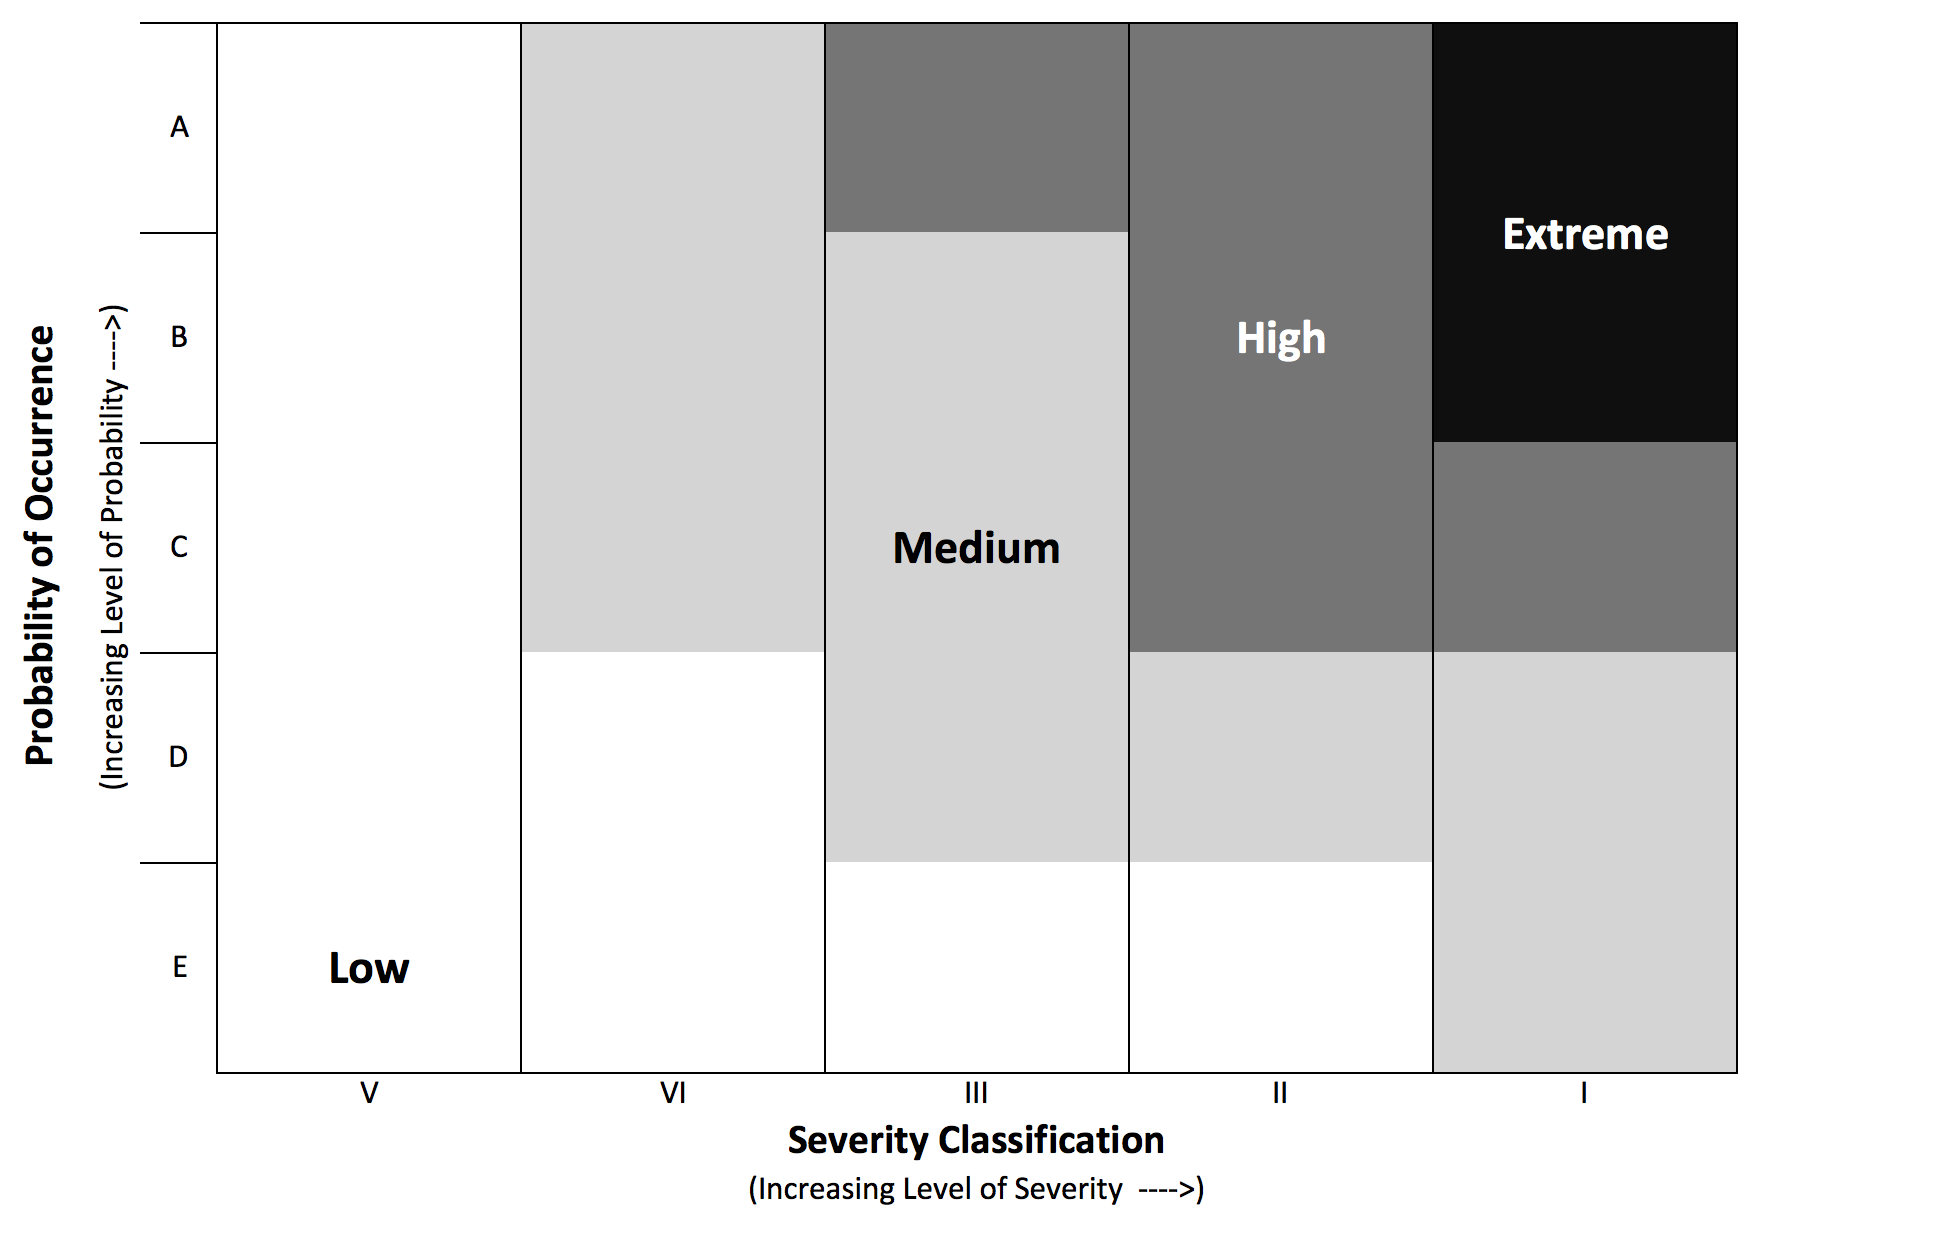
\includegraphics [width=5.5in]{criticalityMatrix2.png}
	\caption{Criticality matrix.}
	\label{fig:critMatrix}
	\end{center}
\end{figure}

In order for the spacecraft to fly all failure modes which land in the extreme and high categories must have their risks mitigated. If the risk isn't mitigated the vehicle customer should be informed of the severity of the risks associated with the mission. Once a risk mitigation is put in place the risk can be re-calculated based on the new criticality. The severity cannot be changed for the failure mode, only the probability that it will happen.

In Appendix \ref{App:FMEA} the entire FMEA is presented with both the original risk and the mitigated risk once some action was taken to reduce the likelihood of that failure mode.

\subsection{Risk Mitigation and Testing}
The final component of the FMEA is to review how risk mitigation actions will be tested, both in simulation and physically.

\subsubsection{Strategies to Mitigate Risk}
There are five strategies to protect against failures: replicated design, diverse design, functional redundancy, temporal redundancy, and information encoding.

Replicating the same design protects against random failures. This involves attaching the same part multiple times so that if one fails, the other(s) can take its place. Since having two of the same sensors will give double information it can be determined if one of them is giving bad information and the other sensor can be used. This strategy has a higher cost, weight and required power, so implementation may be difficult.

Installing two or more components of different design that deliver the same service is referred to as diversifying the design, and increases system redundancy. This redundancy has all the same advantages as replicating the same design, but it can also cover any deficiencies caused by the first design. An example of this is using two types of valves in the main engine design that have different methods of completing the same function. The values have the same function, but can do completely separate things. This implementation introduces additional logistics costs as well as the same costs as replicating design.

Functional redundancy involves using multiple services that give the same information by very different means. An example us using an inertial measurement unit (IMU) and a star tracker to determine the absolute position of the spacecraft. The IMU measures changes in the spacecrafts attitude, and the star tracker measures orientation compared to that of the celestial bodies. They both ultimately deliver attitude information, but can be combined to give more robust information. Another example is using thrusters and a reaction wheel to change the attitude of a spacecraft. While they both change the orientation of the spacecraft, they do so in different means. The problem with functional redundancy is that sometimes there is no alternative way to determine or get the same result. Having the different actuators or sensors can also add extra complexity that must be addressed.

Temporal redundancy involves repetition of an unsuccessful operation. If a computing process is identified as unsuccessful it can be done again to see if a different result is calculated. This can also be applicable in the identification of celestial bodies by the star tracker, by re-doing the calculation a more confident measurement is given. This however is not effective against permanent failures, which will still persist even after the computation is done again.

The final mitigation strategy is information encoding. By encoding the information bits can be lost (specifically due to a single event upset), and the information can be recovered. The correction capability is limits to 1 or 2 bits be event however, so it is not ideal if the mission is in an area with a high chance of single event upsets.

These strategies will be employed to mitigate risk when possible.

\subsubsection{Simulation Testing}
All aspects will have some form of simulation testing done. Because the FMEA revealed many risks associated with proximity operations, one of the largest simulations that needs to be conducted is a rendezvous simulation. This is especially critical because other than flight heritage it is difficult to test rendezvous algorithms. This simulation must prove that the spacecraft is able to rendezvous successfully with one malfunctioning sensor.

\subsubsection{Test Plan}
In order to ensure that the risk mitigation will successfully reduce the risk of some actions physical tests must take place. An example is the launch environment. The launcher provides hazardous longitudinal forces, lateral forces, and vibrations to the spacecraft for a few minutes during launch. The spacecraft must undergo shake table and structural testing to ensure that it will survive the launch environment.

\subsection{Critical Failure Modes}
After completing the FMEA as outlined in the previous section a few items were found to be in the high and extreme risk classification categories. These failure modes can be broken down into a few categories: those that damage Hubble, structural considerations from the launch environment, and surviving the space environment. Failing the mission would be bad, but damaging another spacecraft in the process is unacceptable.

\subsubsection{Rendezvous Risks}
The highlighted risks for damaging Hubble all take place during the rendezvous process. The failure modes include jet fail on, and sensor malfunctions causing an improper docking. Each of these cases must have extensive simulation done to confirm that the failure modes won't result in Hubble being damaged.

To reduce the probability of jet fail and jet fail on, the engine must have redundant valving. These failure modes have orthogonal risk mitigation solutions; however: jet fail requires valves in parallel, and jet fail on requires valves in series. It's possible to do both, that increases overall complexity and adds components to the spacecraft. Since jet fail on has a higher risk, because it can potentially damage Hubble, it is prioritized over the jet fail failure mode. The final result however was to accept the additional complexity, and put the valves in both series and parallel, mitigating risk for both of these failure modes.

Not being able to perceive Hubble's location is also highlighted in the FMEA as a potential mission risk. If Hubble is incorrectly perceived it could lead to a collision during the rendezvous process. To mitigate the risk diverse redundant design is employed. There are different sensors for each piece of information (such as Hubble relative location and reboost vehicle absolute position). This sensor strategy must be tested in simulation to make sure that it's properly working, and successfully reduces the occurrence of incorrectly perceiving information.

\subsubsection{Launch Vehicle Risks}
The launch vehicle provides a large set of problems for the spacecraft including vibrational loading, pressure loading, longitudinal forces and lateral forces. All spacecraft components, and more specifically the structure must be designed to withstand these risks. Prior to launch, all components will be installed into the spacecraft and tested in a simulated launch environment, to ensure that all parts are able to withstand the launch vehicle risks.

\subsubsection{Space Environment Risks}
The space environment has a few items which have high risk identified in the FMEA. These items include the CPU suffering from single event upsets, and orbital debris damaging part of the spacecraft.

In order to mitigate the risk of having single event upsets during critical parts of the mission the spacecraft will be equipped with three CPU's that will vote on actions to take. It's very unlikely that even two of the three CPU's suffer from SEU's at the same time, so by having a simple majority voting scheme the probability of a single event upset giving an incorrect command will be reduced to occurrence level E. This will change the risk to an acceptable level for the mission.

To stop orbital debris from damaging important components the spacecraft will be equipped with micrometeorite and orbital debris shielding. It will be made to withstand MMOD within a probability for occurrence level E. This will reduce the probability of an important system component being hit with debris, and reduce the risk of this failure mode.

%----------------------------------------------------------------------------------------
%	Propulsion
%----------------------------------------------------------------------------------------

\section{Propulsion}

\subsection{Delta V Requirements}
The $\Delta V$ requirements depend largely on the magnitude of the orbital maneuvers required. Therefore, it was necessary to first estimate where the HST will be both at the start of the mission (09/2019), and where it will be approximately 9 years after the reboost, i.e. what altitude is sufficient to extend the HST lifetime to 10/2028. Neither of these can be known precisely, but the latter in particular is subject to a high degree of uncertainty.

To determine where the HST will be, it was necessary to study where it has been. Two Line Element (TLE) data (requested and downloaded from Celestrak~\cite{celestrak}) provided a history of orbital parameters, from the launch date (April 24, 1990) to the present (February 6, 2016). This time period includes multiple past servicing missions, some of which included small reboosts.

The parameter of greatest interest to the mission was the mean altitude (h) over time. This was calculated by using the mean motion ($n$), converted from revs/day to rad/s, to find the semi-major axis ($a$) of the ellipse
\begin{align*}
h = a - r = \sqrt[3]{\mu/n^2} - r
\end{align*}
where $\mu = \mu_{earth} = 3.986$ x 10$^14$ m$^3$/s$^2$ and $r = r_{earth} = 6.378$ x 10$^6$ m. The result is shown in Figure~\ref{fig:fig1} below.

\begin{figure}[H]
\begin{center}
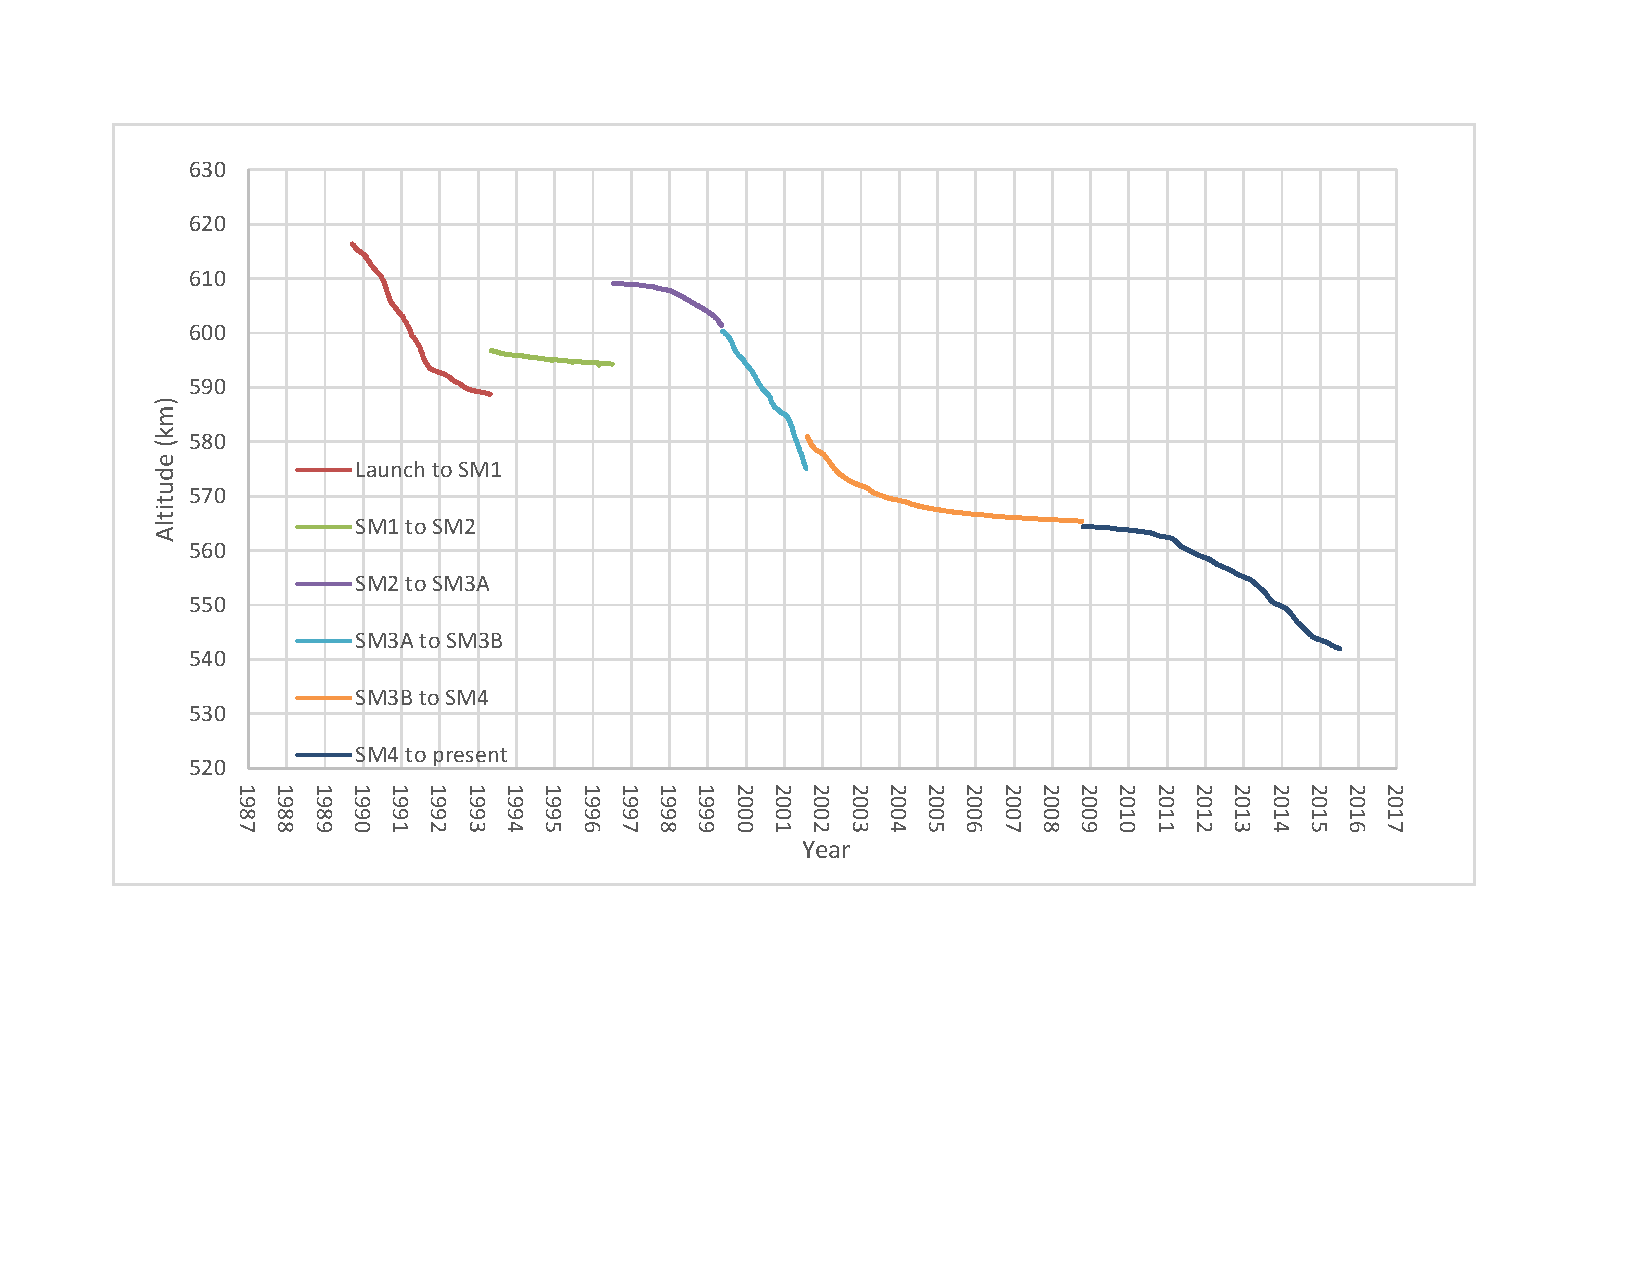
\includegraphics[width=1\textwidth]{figs2/1.pdf}
\caption{Mean HST Altitude vs. Year.}
\label{fig:fig1}
\end{center}
\end{figure}

As Figure~\ref{fig:fig1} shows\footnote{Note that the x-axis lines and labels displayed represent the midpoint of each year (approximately July 2 rather than January 1).}, the orbital decay of the satellite is not constant. The largest factor in the decay at this altitude is atmospheric drag, which itself is dependent on the solar cycle. During periods of increased solar activity, which can be approximated by the number of sunspots observed, the atmospheric density can be up to two orders of magnitude greater. This leads to a larger drag force on the satellite. Solar cycle data was obtained from monthly averages of the daily sunspot number, and plotted alongside the HST altitude history~\cite{sunspots}.

As shown in Figure~\ref{fig:fig2} and Figure~\ref{fig:fig3}, the changes in number of sunspots correlates to the historical rate of change of orbital decay for the HST.

\begin{figure}[H]
\begin{center}
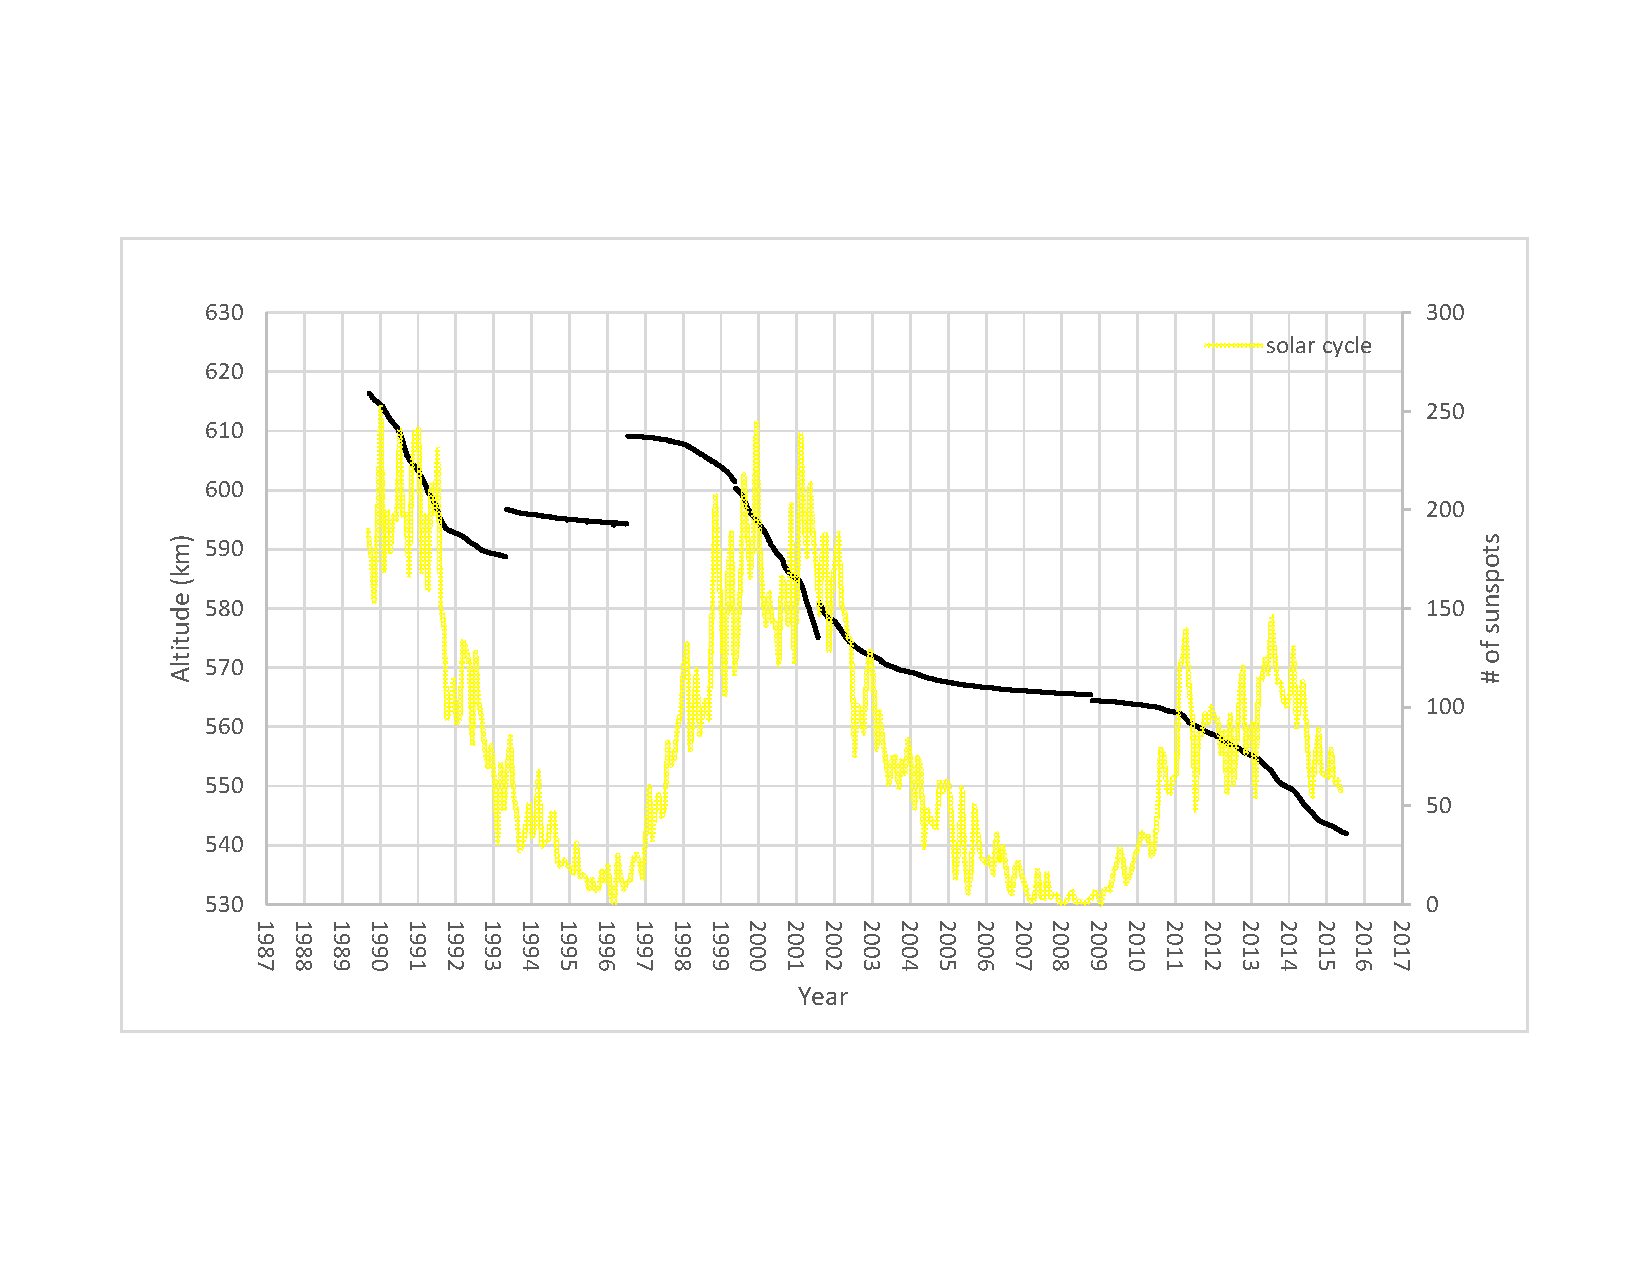
\includegraphics[width=1\textwidth]{figs2/2.pdf}
\caption{Mean HST Altitude \& Solar Cycle vs. Year.}
\label{fig:fig2}
\end{center}
\end{figure}

The rate of change of altitude can also be calculated using the TLE data, assuming that the orbit is approximately circular. Differentiating with respect to time (using the chain rule) gives the following
\begin{align*}
\dfrac{d}{dt} h = \dfrac{d}{dt} a = \dfrac{da}{dn} \dfrac{dn}{dt} = \dfrac{d}{dn} \mu^{\sfrac{1}{3}} n^{-\sfrac{2}{3}} \dfrac{dn}{dt} = -\dfrac{2}{3} \mu^{\sfrac{1}{3}} n^{-\sfrac{5}{3}} \dfrac{dn}{dt}
\end{align*}
where $\frac{dn}{dt}$ is also given by the TLEs. Therefore, rate of change of altitude ($\frac{dh}{dt}$) can also be plotted versus time and compared to the solar cycle data, as shown in Figure~\ref{fig:fig3}. Despite a large amount of transient error propagated through this calculation, there is a clear correlation between $\frac{dh}{dt}$ and the sunspot number.

\begin{figure}[H]
\begin{center}
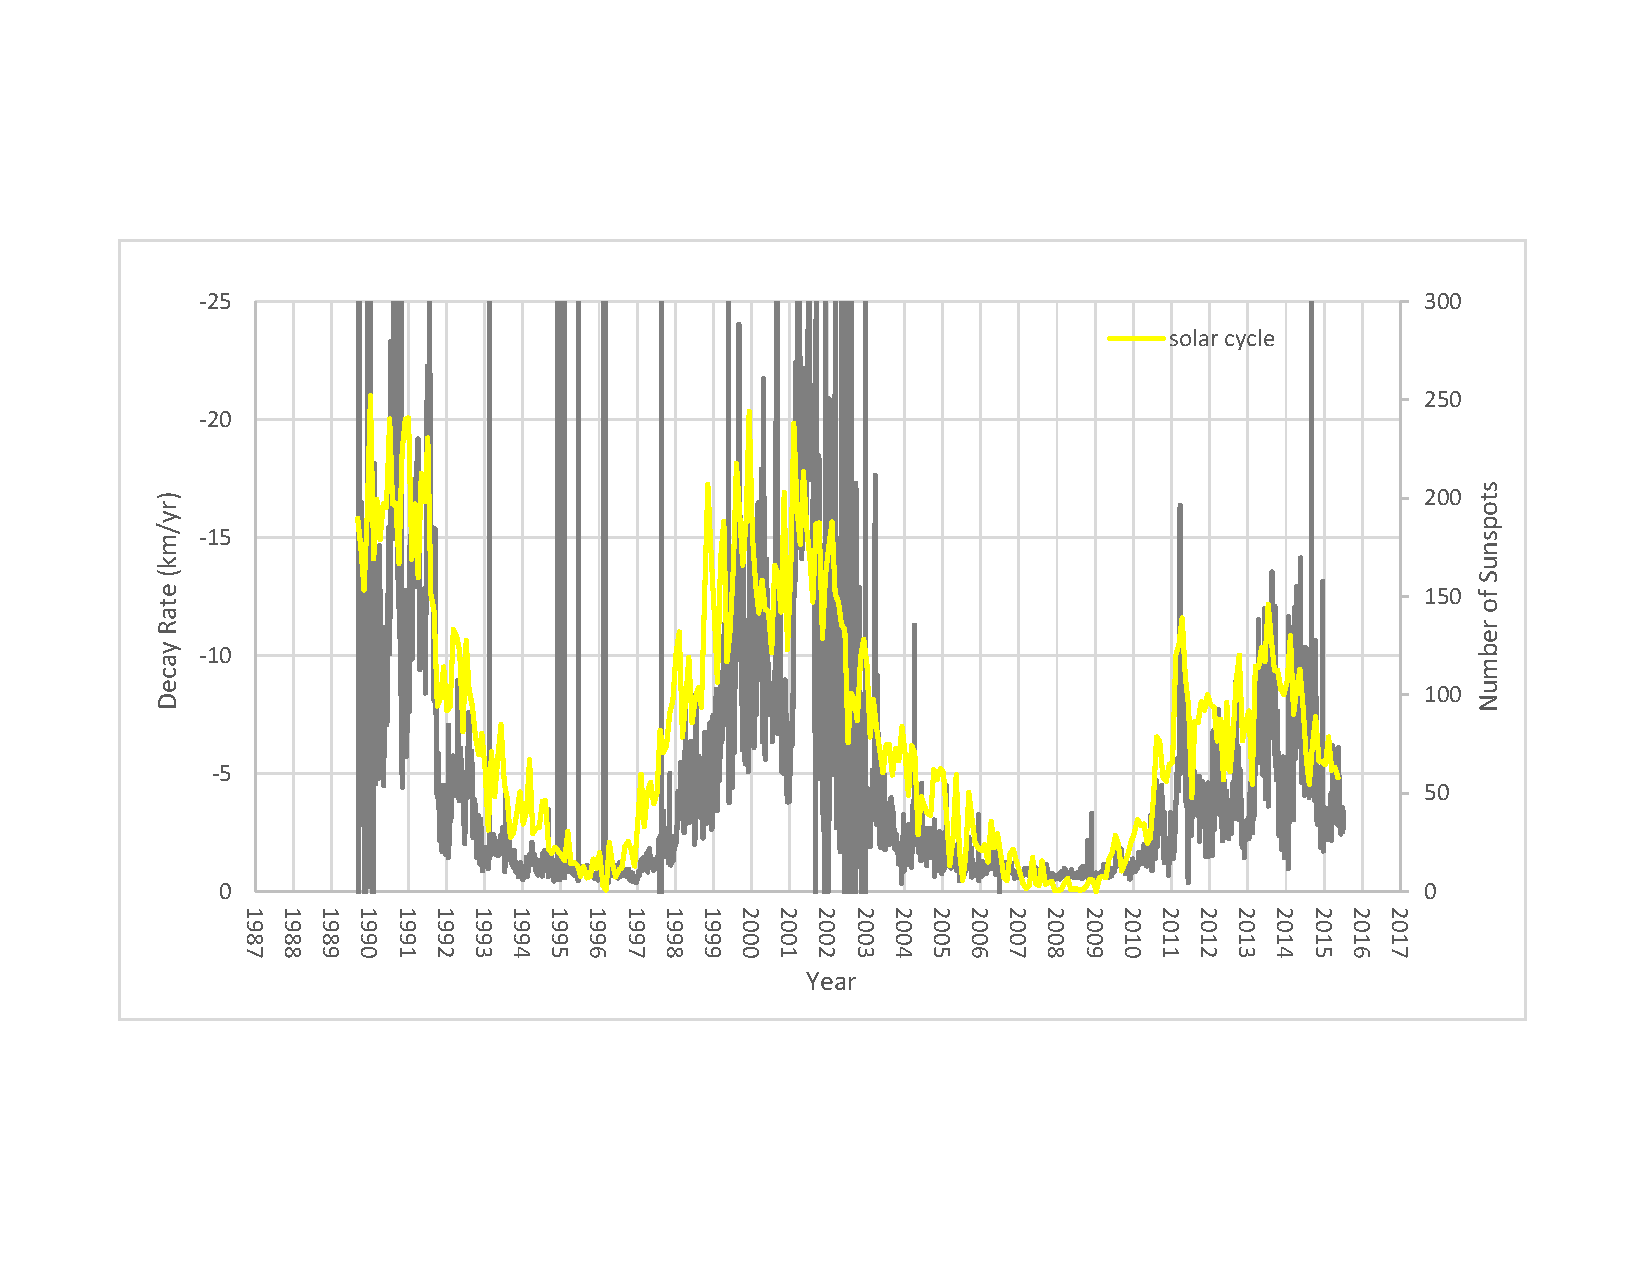
\includegraphics[width=1\textwidth]{figs2/3.pdf}
\caption{Mean Altitude Decay \& Solar Cycle vs. Year.}
\label{fig:fig3}
\end{center}
\end{figure}


\subsubsection{2020 Prediction}
The current solar cycle is significantly weaker than the previous two cycles, and appears to have already peaked. Therefore, it is expected that the HST orbital decay rate in the next few years will not be large. Figure~\ref{fig:fig3} shows that during periods of low solar activity, the decay rate can be as low as a kilometer per year. However, there is still a fair amount of uncertainty with regards to the future solar output and its effect on the satellite orbit, as hinted at by the amount of noise in the graph. Therefore, it would be wise to adopt a conservative approach during the preliminary design phase.

The HST altitude data was fitted in a few different ways in order to project to 2020. If the current decay rate were to continue with no decrease in solar cycle, the altitude would be 528 km --- however, this is an overly conservative estimate. If the decay rate matched that of the previous low periods, the altitude would be 536 km --- however, the previous periods were at a slightly higher altitude and this may not be steep enough, since decay rate decreases with altitude. Both of these scenarios are shown in Figure~\ref{fig:fig4}.

\begin{figure}[H]
\begin{center}
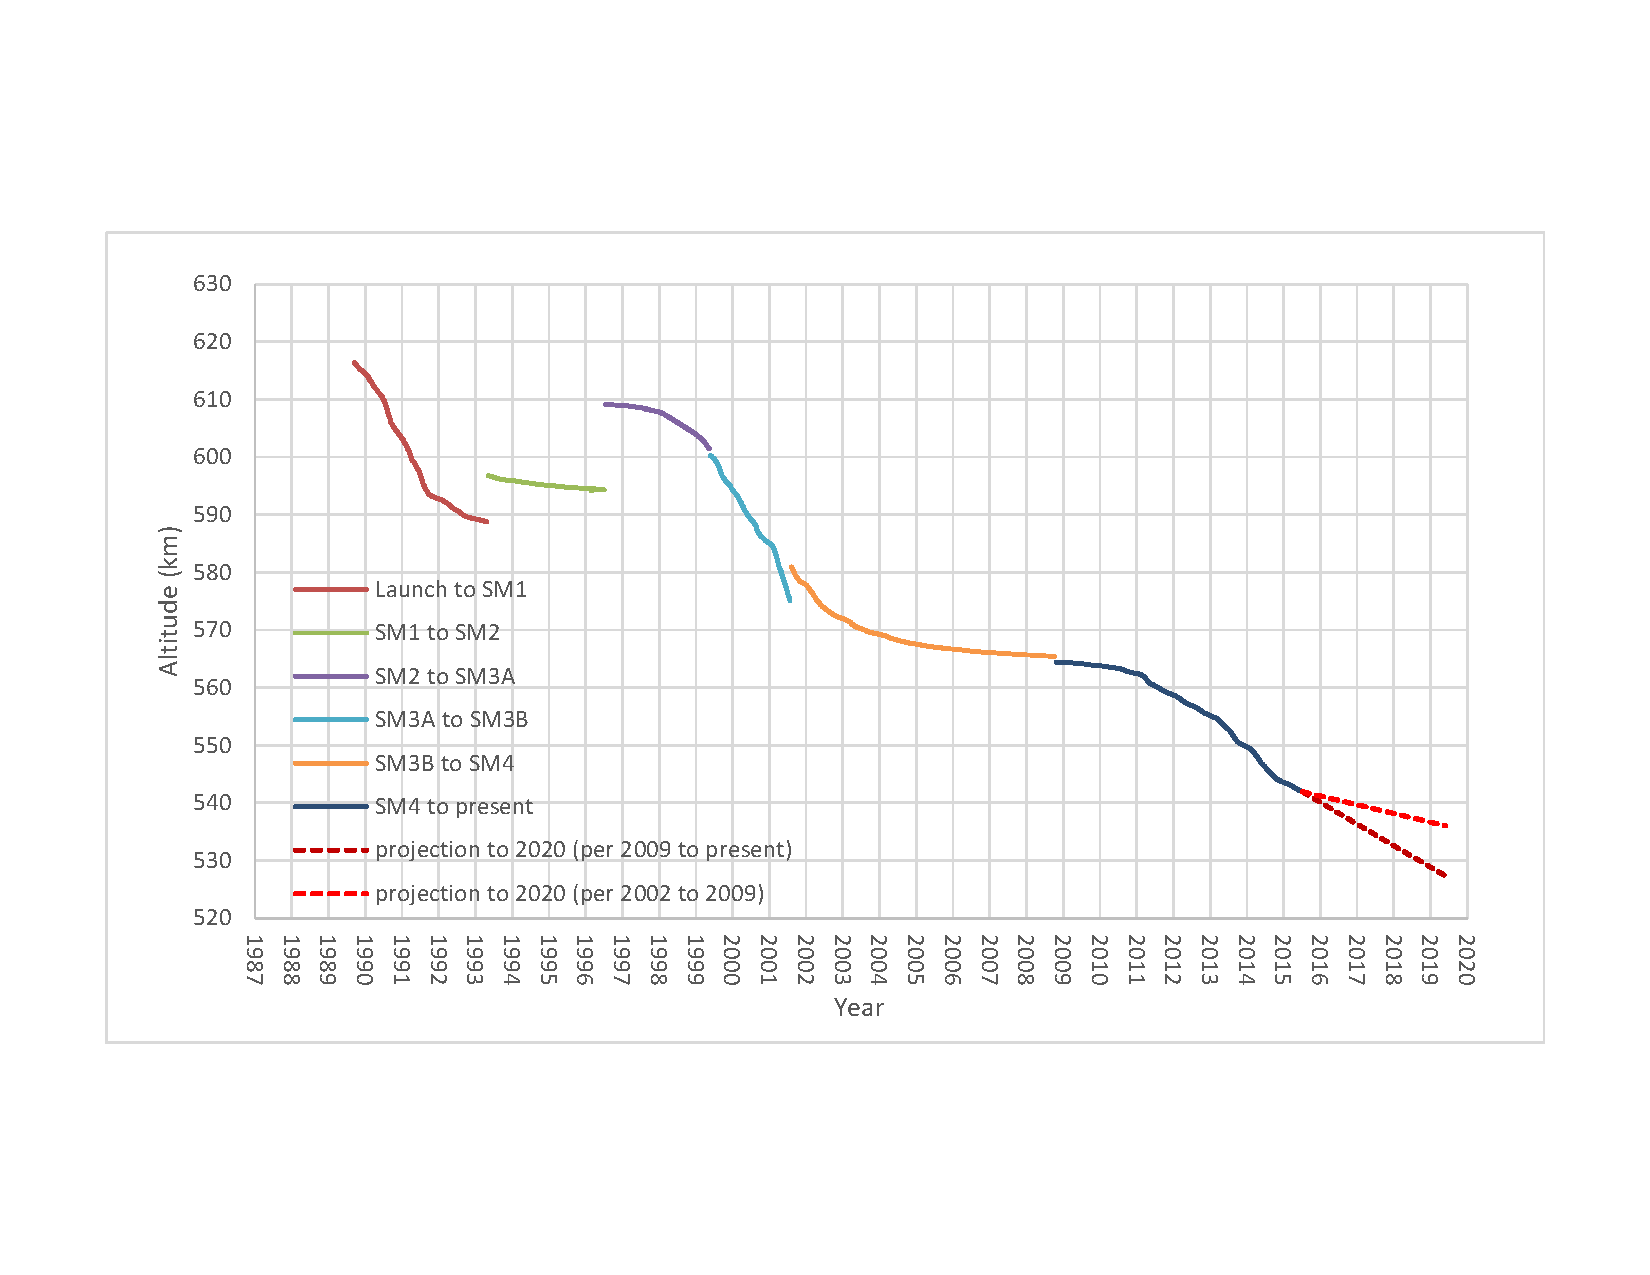
\includegraphics[width=1\textwidth]{figs2/4.pdf}
\caption{Projected Change in Altitude.}
\label{fig:fig4}
\end{center}
\end{figure}

An additional analysis was performed using AGI's Systems Took Kit (STK) software. STK was used to calculate the orbital elements for the HST from the present to 2028. The STK analysis did not account for a changing solar cycle model, but instead used a drag estimate for the mean solar output. The STK model predicted a semi-major axis of 6910 km, corresponding to an altitude of 532 km in 2020, as shown in Figure~\ref{fig:fig5}.

\begin{figure}[H]
\begin{center}
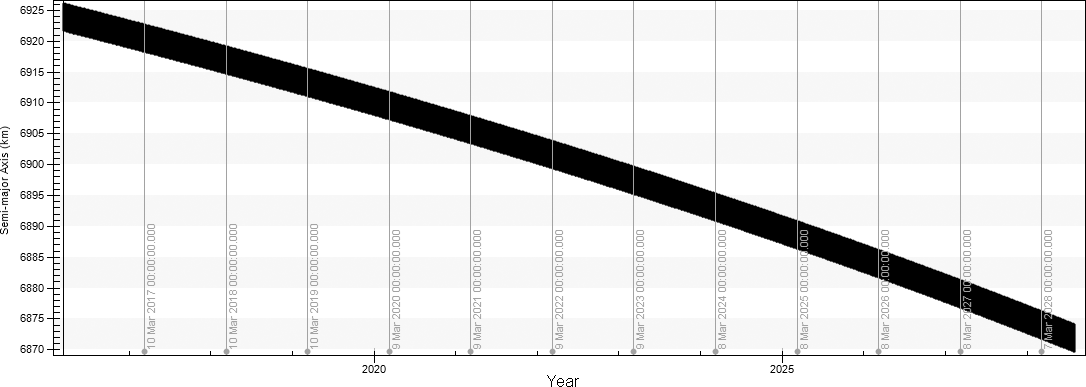
\includegraphics[width=1\textwidth]{figs2/5.png}
\caption{STK Altitude Prediction.}
\label{fig:fig5}
\end{center}
\end{figure}

The STK prediction falls neatly between the two previous predictions, therefore this altitude (532 km) was chosen for the mission.


\subsubsection{2028 Prediction}

The mission requirement is to reboost the HST to a sufficient altitude so that it survives to October 2028. This involves predicting the decay rate at a number of possible reboosted altitudes. However, future predictions become more difficult as the length of time is increased --- the solar cycle in particular is not easily predictable.

Figure~\ref{fig:fig5} also shows the HST altitude if no reboost was done, which leads to the question of whether the reboost is even necessary. Another solar maximum will occur during this time frame, though the exact change in solar output is unknown. However, even without knowing the precise solar output over the next cycle, it appears likely that the HST could survive to 2028 on its own. This is partially due to the exceptionally weak current solar cycle.

Considering Hubble's history and considerable value even after the JWST is operational, it is desirable to continue HST's operation as long as possible. The HRV's sole purpose is reboosting the HST and it must be designed large enough to interface with the HST regardless of the actual altitude. Because of these factors, it was decided to reboost the HST as high as possible---back to its initial deployed altitude of 616 km. This will ensure the continuous operation of the HST to 2028 and well beyond.

\subsection{Orbital Mechanics}

All orbits for the mission were initially modeled as simple Keplerian orbits with no perturbations. All transfers (with the exception of rendezvous, dock \& undock) were initially modeled as simple Hohmann transfers. Therefore, the orbital velocities and transfer $\Delta V$'s were easily calculated from the semi-major axes using

\begin{align*}
V = \sqrt{\dfrac{\mu}{\dfrac{2}{r}-\dfrac{1}{a}}}
\end{align*}

Estimates of the propellant mass required were done using the Tsiolkovsky rocket equation,

\begin{align*}
\Delta V = I_{sp} g_0 \ln \dfrac{m_i}{m_f}
\end{align*}
where the propellant mass is given by $m_i-m_f$. The engine $I_{sp}$ and dry mass of the HRV were estimated for the initial calculations.

This model was iterated over time as the subsystem designs evolved and the mass estimates were refined. The final result is shown in Table~\ref{table:delta_vs}. Rendezvous and dock are accomplished using cold gas thrusters in order to prevent damage to the HST. Therefore, this propellant is calculated with a lower $I_{sp}$ and tabulated separately. The fuel required for the evasive maneuver is calculated at the beginning of the mission, but not subtracted from the spacecraft mass. In the event that no evasive maneuver is required, this extra fuel will be carried for the duration of the mission, which represents the ``worst case'' scenario with regards to the other transfer maneuvers.

\begin{table}[H]
\begin{center}
\begin{tabular}{rrrrrrrrrr}
\toprule
Mission Phase & Total $\Delta V$ (m/s) & Prop. Mass (kg) \\
\midrule
Deorbit & 				    140 & 					38 \\
Reboost & 					46  & 					210 \\
Rendezvous \& Dock &       	25	& 					36 \\
Parking to HST & 			207 & 					78 \\
Evasive Maneuver & 			150 & 					57 \\
\bottomrule
\end{tabular}
\end{center}
\caption{$\Delta V$'s and Propellant Masses.}
\label{table:delta_vs}
\end{table}


For this stage of the design process, an extra 20\% propellant (all types) was added to the final spacecraft mass. The cold gas thrusters are also used for desaturation of reaction wheels, requiring additional mass of cold gas. The final masses for the mission are given in Table~\ref{table:final_masses}.

\begin{table}[H]
\begin{center}
\begin{tabular}{ll}
\toprule
Dry Spacecraft & 617 kg \\
Total Propellant & 502 kg \\
Launch Mass & 1,118 kg \\
Deorbit Mass & 757 kg \\
\bottomrule
\end{tabular}
\end{center}
\caption{Final mission masses.}
\label{table:final_masses}
\end{table}

\subsection{Selection of Main Engine}
The performance of the main engine was constrained by several requirements. While it may be possible to gradually reboost the HST with a small engine, a long, slow orbit change could put the HST at a greater risk of collision with debris, and possible increased risk of contamination from the engine exhaust. A Hohmann transfer was chosen in order to provide the fastest and most efficient maneuver. Therefore, all engine firings must be sufficiently short (burn time $\ll$ orbital period) to be modeled as impulse maneuvers.

The engine has to have sufficient power to change the orbit of the vehicle with the HST attached. The HST was represented by an estimated mass of 12,273 kg (27,000 lbs), which requires a significant amount of thrust to accelerate. However, in order to protect the HST, the maximum thrust is limited by the boom deflection customer requirement (d).

A number of thrusters were considered in seeking to balance these constraints. Many engines were capable of a slow reboost, however, the burn time was anywhere from 25\% to 100\% of the transfer time---clearly not an impulse maneuver. This lower bound was found to be more constraining, as few engines produces critically high accelerations, due to the large mass of the HST.

\subsection{Propellant Type}

The most significant design decision regarding the propulsion system was the choice between a monopropellant or bipropellant engine. The advantages of monopropellant engines are simplicity and high reliability. However, most designs have a lower ceiling for maximum thrust and $I_{sp}$. Bipropellant engines are typically available in higher thrusts and better $I_{sp}$'s, but the increased complexity can make them less reliable. Using two tanks is also inherently less mass efficient, however, the higher $I_{sp}$ can easily make up for this, as well as for the additional valves and plumbing required.

A review of common engines revealed that only one monopropellant option (Aerojet MR-80B) generates the amount of thrust (3,780 N) necessary for impulse maneuvers with the HST attached~\cite{monoprop}. While this engine would seem to be a good fit for the mission, it was unwise at this stage of the planning process to commit to a design choice with only one supply option. A number of bipropellant engines were capable of meeting the operational requirements, most of which have established flight histories and have been proven to be reliable. Therefore, the choice was made to design for a bipropellant system.

The bipropellant engine chosen for the mission was the Aerojet R-40B, a variant of the thrusters used on the space shuttle, albeit with a more conventional design~\cite{biprop}. The R-40B uses a monomethylhydrazine (MMH) fuel and a nitrogen tetroxide (NTO) oxidizer. The engine has a high specific impulse of 293 s, a low mass of 7.23 kg, and a maximum thrust of 4,000 N. This thrust corresponds to a maximum acceleration (with HST attached) of 0.3 m/s$^2$, and a burn time of about 76 seconds, which meets both the upper and lower requirements for the engine.

\subsection{Propellant Tank Sizing}

The tanks used for the fuel and oxidizer are sized according to the volume of fuel required, including the 20\% margin. A curve fit model for typical diaphragm propellant tank masses was used to estimate the tank masses~\cite{ref12_8}.

The R-40B engine is pressure driven, and the propellant tanks will be pressurized by two external pressurant tanks. Traditional diaphragms are planned for use rather than propellant management devices (PMDs). While PMDs provide a number of benefits, and could be a good fit for the low accelerations and short maneuvers required by this mission, the established design of the diaphragms is still more favorable.

\subsection{Pressurant Tank Sizing}

Two cross-fed pressurant tanks will be used to pressurize the propellant tanks and feed the fuel and oxidizer to the engine. The pressurant tanks were sized according to the pressurant type, Helium, and an assumed beginning-of-life (BOL) pressure of 21 MPa (3,000 psi). While helium pressurant has a lower density than nitrogen, the tanks will be small enough to negate this concern. The low molecular density is an advantage in that the helium pressure is less sensitive to temperature changes than nitrogen.

The R-40B engine requires a minimum pressure of 1 MPa to operate. The pressurant must completely fill the propellant tanks at this end-of-life (EOL) pressure. Assuming no temperature rise (a worst-case condition regarding the pressure), 0.69 kg of Helium is required. Two metallic tanks, 3.5 kg each, will be used to contain the pressurant.

It would also be possible to use COPV tanks for the mission. Metallic tanks are typically more robust and reliable, but COPV tanks could perform the same function with less mass. However, for the relatively small tanks required for the mission (less than 1 m in diameter), metallic tanks are still a reasonable option. The mass savings from using COPV was not deemed sufficient to warrant the increased risk.

\subsection{Valves and Plumbing}

\begin{figure}[H]
	\begin{center}
	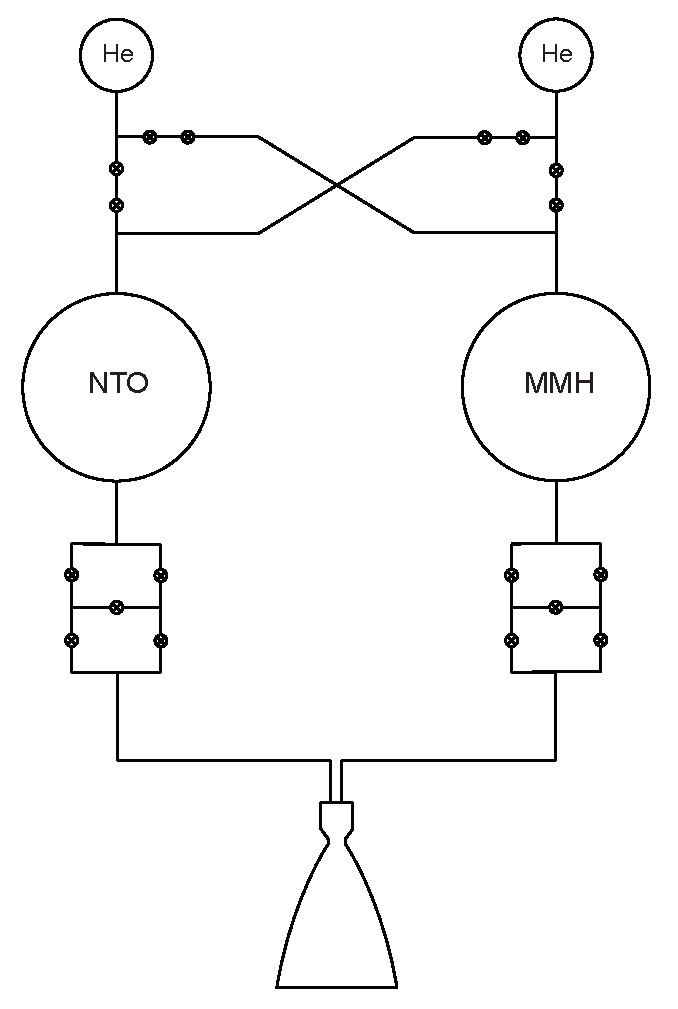
\includegraphics[height=.4\textheight]{propellant_system_diagram.pdf}
	\caption{Propellant system diagram.}
	% \label{fig:ballisticLimitStructure}
	\end{center}
\end{figure}

\begin{figure}[H]
	\begin{center}
	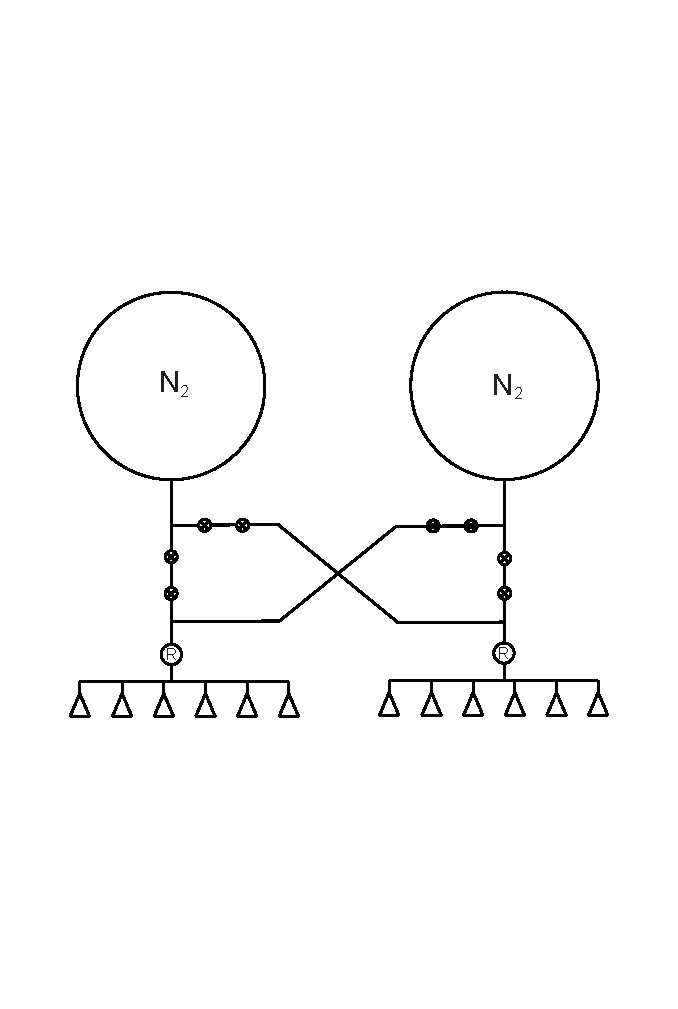
\includegraphics[height=.35\textheight]{cold_gas_system_diagram.pdf}
	\caption{Cold gas system diagram.}
	% \label{fig:ballisticLimitStructure}
	\end{center}
\end{figure}

A regulated system including redundant series and parallel valves will be used to feed each pressurant tank to the propellant tanks and each propellant tank to the engine. This will protect against any single valve failure, either open or closed. Preventing jet-on fail in particular is crucial to the mission. Due to the delicate proximity operations required by the cold gas thrusters, they will be fed with a passive regulated system.

\subsection{Cold Gas}

Cold gas thrusters will be used both for attitude control and rendezvous maneuvering. While it would be simpler to have a single bipropellant system feeding both the main engine and the smaller thrusters, the sensitive nature of the HST prohibits the use of hydrocarbon fuels when nearby.

Cold gas thrusters typically use nitrogen or helium, and have a thrust of a few Newtons and an ISP of about 70 s. Refer to the attitude control section for the thrusters chosen for the mission. For redundancy and better mass distribution, two identical cold gas tanks were used. The cold gas tanks are approximately the same size and volume as the propellant tanks.

The tank mass was determined by the maximum pressure ($p$), radius ($r$) and allowable stress ($\sigma$) for the material type according to the following estimation
\begin{align*}
t = \dfrac{p r}{2 \sigma}
\end{align*}
where $t$ is the thickness of the tank walls. By using 7075-T73 Aluminum for the tank material, the tanks have a thickness of about 1 cm, and a total mass of approximately 43 kg each. This estimate assumes a maximum pressure of about 21 MPa.

\subsection{Phasing}

Two stages of the mission requires phasing---rendezvousing with the HST and deorbiting over the ocean rather than land. Both of the requirements will be met with careful timing rather than forced maneuvering.

The launch time will be chosen so that the HRV lags the HST's true anomaly by a small amount. At the parking orbit or 200 km, the HRV will orbit slightly faster than the HST, slowly catching up to it. The HRV will transfer to the HST orbit after a specified ``wait time'', chosen to allow rendezvous during the day.

After the reboost, the HRV will use the spring force of the docking mechanism to slowly drift away from the HST, aided by the cold gas thrusters if necessary. At this phase, the HRV is able to remain at the reboosted altitude for multiple orbits. The HRV will time the slowdown burn in order to deorbit over the ocean.

Therefore, no additional propellant is needed to meet the phasing requirements. The amount of propellant needed to overcome orbital perturbations for the altitudes and durations specified is negligible, as shown in Section~\ref{howlong}.

\subsection{Test Plan}
The main engine and the cold gas thrusters will be tested to ensure that they perform according to specification and to reduce the risk of manufacturing defects leading to infant mortality. The main engine and all thrusters will be subjected to a simulated launch environment, followed by test fires. The test fires will be done on a fixture to measure thrust and verify performance. To verify operation of the propellant delivery system, valves will be intentionally failed open or closed at random.  The continued operation of the thrusters will verify that no single failure is capable of causing a jet fail on or jet fail off. All propellant and pressurant tanks shall be subject to a simulated launch environment, followed by proof pressure tests.


%----------------------------------------------------------------------------------------
%	Rendezvous
%----------------------------------------------------------------------------------------

\section{Rendezvous}

\subsection{Docking}
\subsubsection{Small Autonomous Satellites}
There have been incredible advancements within the realm of semi-autonomous satellites over the past 20 years. Beginning in 1997, the Autonomous Extravehicular Activity Robotic Camera Sprint (AERCam Sprint) was the first semi-autonomous satellite to demonstrate the use of a free-flying prototype camera aboard the International Space Station (ISS). While operating alongside STS-87 Mission Specialist Winston Scott, the AERCam Sprint flew under the remote-control guidance of Steve Lindsey for approximately 75 minutes, and relayed live television images to Columbia's Mission Control~\cite{Aercam,MiniAercam}. After successfully completing this experiment, researchers and analysts decided to incorporate a higher level of autonomy, and produced a second prototype known as the Mini AERCam in 2000. While this satellite never made it to space, the Mini AERCam underwent multiple tests on an air-bearing table and in an orbital test simulation facility at Johnson Space Center. This newly designed satellite was given automatic position hold, point-to-point maneuvering, and an additional camera to provide an orthogonal view, allowing astronauts to navigate the Mini AERCam with respect to the ISS. Through these multiple additions, researchers expanded the satellite's capability to encompass supervised autonomous and/or remotely piloted operations~\cite{MiniAercam,MiniAercam2}.

In 2006, the first Synchronized Position Hold Engage Reorient Experiment Satellites (SPHERES), a self-contained nanosatellite made by MIT's Space Systems Laboratory, was launched to the ISS and taken to the US Laboratory. Since that time, this semi-autonomous satellite has been joined by two additional SPHERES, making this system the first consistent experimental nanosatellite testbed aboard the ISS. Unlike the AERCam Sprint and the Mini AERCam, SPHERES is a modular satellite where each system is self-contained in individual capsules. This configuration allows SPHERES to easily incorporate system expansions onto specific platforms, such as navigation, without needing to reconfigure the entire craft. Furthermore, its modularity helps researchers efficiently address system failures, making it easier for astronauts to perform on-site repairs.

To navigate SPHERES within the ISS, the system utilizes wall-mounted ultrasonic beacons and corresponding ultrasonic receivers attached to the nanosatellite~\cite{SPHERES}. SPHERES emits an infrared flash to determine its location. Once emitted, the satellite waits for the wall-mounted beacons to emit corresponding ultrasonic pulses. After receiving these ultrasonic pulses, the satellite measures its range based on the pulse's time of flight, and can then calculate its relative position, attitude, and angular velocity~\cite{SPHERES,Vertigo1}. This unique navigation system allows SPHERES to emulate a ``pseudo-GPS'' time-of-flight sensing system, and ultimately estimate its position, angular velocity, and attitude without the potential for signal interference and noise -- a challenge that has been previously encountered with GPS systems~\cite{Vertigo1}. Through this autonomous navigation and modular design, the SPHERES testbed has become a versatile platform for developing vision-based navigation, anti-collision, and formation flying algorithms. By allowing research teams to create algorithms that can then be uplinked to the SPHERES test system aboard the ISS, researchers can receive live feedback, and ultimately find the exact areas within their algorithms that need improvement.

In 2008 the MIT Space Systems Laboratory began building an upgrade to the SPHERES system, known as the Low Impact Inspection Vehicle (LIIVe), as part of the Visual Estimation and Relative Tracking for Inspection of Generic Objects (VERTIGO) program. Once completed, this upgrade would later be attached to the existing SPHERES system and act as VERTIGO ``goggles,'' allowing SPHERES to perform vision-based navigation experiments in the microgravity environment aboard the ISS. After adjusting these VERTIGO Goggles to suit the space station's environment, the final system was upgraded to include two monochrome stereo cameras, two illuminating LEDs, a 1.2 GHz Via Nano processor, an 802.11n network card, and optics that included a larger aperture lens in a synchronized stereo configuration~~\cite{SPHERES,Vertigo1,Vertigo2,Vertigo3}.

When the modified SPHERES VERTIGO was ready for experimentation, numerous flight algorithms were tested to demonstrate the spacecraft's complete autonomy. After ISS Expedition 34, it was confirmed that SPHERES VERTIGO was capable of autonomously conducting a circular orbit about an uncooperative object, while simultaneously maintaining a constant relative position between SPHERES VERTIGO and the target. This objective was achieved through the primary use of inertial sensors and cameras, and was considered an unprecedented success~\cite{Vertigo2,Vertigo3}.

\subsubsection{Collision Avoidance and Docking Algorithms}
Since the SPHERES nanosatellite's first microgravity guidance, navigation, and control experiment, there have been three classes of algorithms pertaining to collision avoidance and docking that have emerged: metrology, control, and autonomy~\cite{SPHERES_form}.

The metrology algorithms were implemented using a SPHERES-specific interface, and utilized a series of Extended Kalman Filters to obtain the system's state vector from the sensor outputs. This approach has been typically utilized in position, attitude, and determination systems. Despite many successful implementations, recent literature suggests that the second and third classes have demonstrated greater accuracy in the areas pertaining to collision avoidance and docking~\cite{SPHERES_form}.

The control algorithm class involves both closed-loop controls and path-planning algorithms. One prominent control algorithm that has been frequently tested is the glideslope algorithm. This algorithm is a hybrid between a path-planning and a velocity-control algorithm, where the incoming spacecraft is given commands to slow its velocity as it approaches its target~\cite{SPHERES_form,SPHERES_micro,dist,virt_sim}. The glideslope algorithm was the first autonomous docking algorithm to successfully attach an incoming spacecraft to its tumbling target, and is a relatively simple, yet robust, controller algorithm~\cite{SPHERES_micro}.

Another promising algorithm is the ``safe'' trajectory algorithm. This innovative algorithm computes a pre-planned trajectory using the solution from a Mixed-Integer Linear Program, and, using this pre-computed trajectory, is able to optimize fuel and avoid incoming obstacles~\cite{SPHERES_micro}. However, while this algorithm is guaranteed to produce a safe trajectory, its overall complexity requires it to be computed on an external computer. Once the computations have been completed, the final trajectory is transferred to the satellite. This entire computational process creates an approximate nine second delay, and can potentially create a catastrophic outcome if the spacecraft requires an immediate trajectory path to avoid an incoming collision. To remedy this solution, researchers have begun to trade trajectory and fuel optimality for computational time, and can reduce the total computation time to about $0.17$ seconds~\cite{SPHERES_micro}.

Lastly, the ``close point of approach'' algorithm has been demonstrated to be both compact and computationally efficient, and has served as a background safety routine for the high school SPHERES Zero Robotics program~\cite{virt_sim}. While all three aforementioned algorithms have accurately performed numerous tests pertaining to collision avoidance and docking, each algorithm is associated with its own specific set of pros and cons. As it currently stands, researchers have yet to find a way to optimize fuel usage, pre-planned trajectories, and computational power, and thus must decide which factors are most important for any given mission~\cite{SPHERES_form,SPHERES_micro,dist,virt_sim}.

Finally, the autonomous algorithm class is used to execute the control class algorithms and determine the current mode of operation~\cite{SPHERES_form}. As a result, the glideslope, ``safe'' trajectory, and ``close point of approach'' algorithms all utilize autonomy to properly perform their respective procedures.

\subsubsection{Autonomous versus Manual Docking}
In recent years the small satellite platform has increased in popularity. With the ability to launch multiple small satellites as a secondary payload and the relatively low development cost involved, they are one of the most viable testbeds for new technologies. One great example of this is the class of satellites that adhere to the CubeSat standard~\cite{CubeSat}. CubeSat initiatives have made many projects possible due to the minimal costs required. Although a small size limits their capabilities, higher fidelity projects usually require a larger volume to contain all desired systems. There are several projects that use slightly larger free flyers that have produced unique navigation demonstrations such as AERCam Sprint, Mini-AERCam, and SPHERES ~\cite{Aercam,MiniAercam,SPHERES}. While the Hubble Reboost Vehicle (HRV) is significantly larger than the aforementioned satellites, the rendezvous and docking algorithms developed for these missions can be made just as effective.

These projects make use of an optical sensor to take stereoscopic visual recordings for inspection purposes, and to determine the position and attitude in relation to a target. To do this, the image captured must be used in conjunction with a computer vision algorithm in order to estimate navigational parameters. Using two color cameras and the full visual light spectrum, a more familiar virtual image is produced. Operators are able to view the subject as if it was in front of them, allowing for quick and informed decision making. This, as among other reasons, has been realized by many research teams and can be seen in many projects such as SPHERES VERTIGO and the aforementioned AERCam projects~\cite{Aercam,MiniAercam,Vertigo1}.

Most current docking procedures utilize a laser range finder for determining distance. Laser range finders have flight heritage and have moderate accuracy~\cite{Docking}. Simple fiducial markers can be used to increase the performance of range finders, and multiple markers can allow rangefinders to triangulate a relative position. Markers for visual navigation systems, however, can vary in complexity. Marker distribution and marker shape can allow a computer vision system to gather a large amount of data with a single image, whereas a laser rangefinder must take multiple measurements. This system was originally developed for manual docking operations, but it also provides visual information to allow more accurate computer vision position measurements.

In ground-based scenarios, the only drift from the intended rendezvous trajectory is contributed to error or disturbances, but in this situation there is also drift due to the inspector and the target occupying different orbits. Even with a perfect initial trajectory and planning, corrections are required. The navigation scheme must be as efficient as possible as course corrections are unavoidable.

The great distances involved in satellite operation, coupled with an inherent delay involved with routing signals to a ground station, however, make human operation of the HRV infeasible. A one-way time delay of a few seconds from a satellite to the ground-based operator, with the addition of just one second of human operator delay, with the additional delay of a few seconds back from the ground-based operator to the satellite result of time delays greater than 5-10 seconds, at which point it is too late to make corrections. An automated system, based on the navigation schemes outlined above, has a much greater chance for success. Such a system can make nearly instantaneous decisions, and can execute them before a human operator has time to identify the situation. Coupling an automated docking procedure with a human backup to abort gives the best of both scenarios. The automated docking system can handle the lower level task of docking, and the human operator is present to abort the docking attempt if unexpected errors occur.

\subsection{Rendezvous}

\subsubsection{How will we rendezvous?}
\begin{figure}[tbh!]
\begin{center}
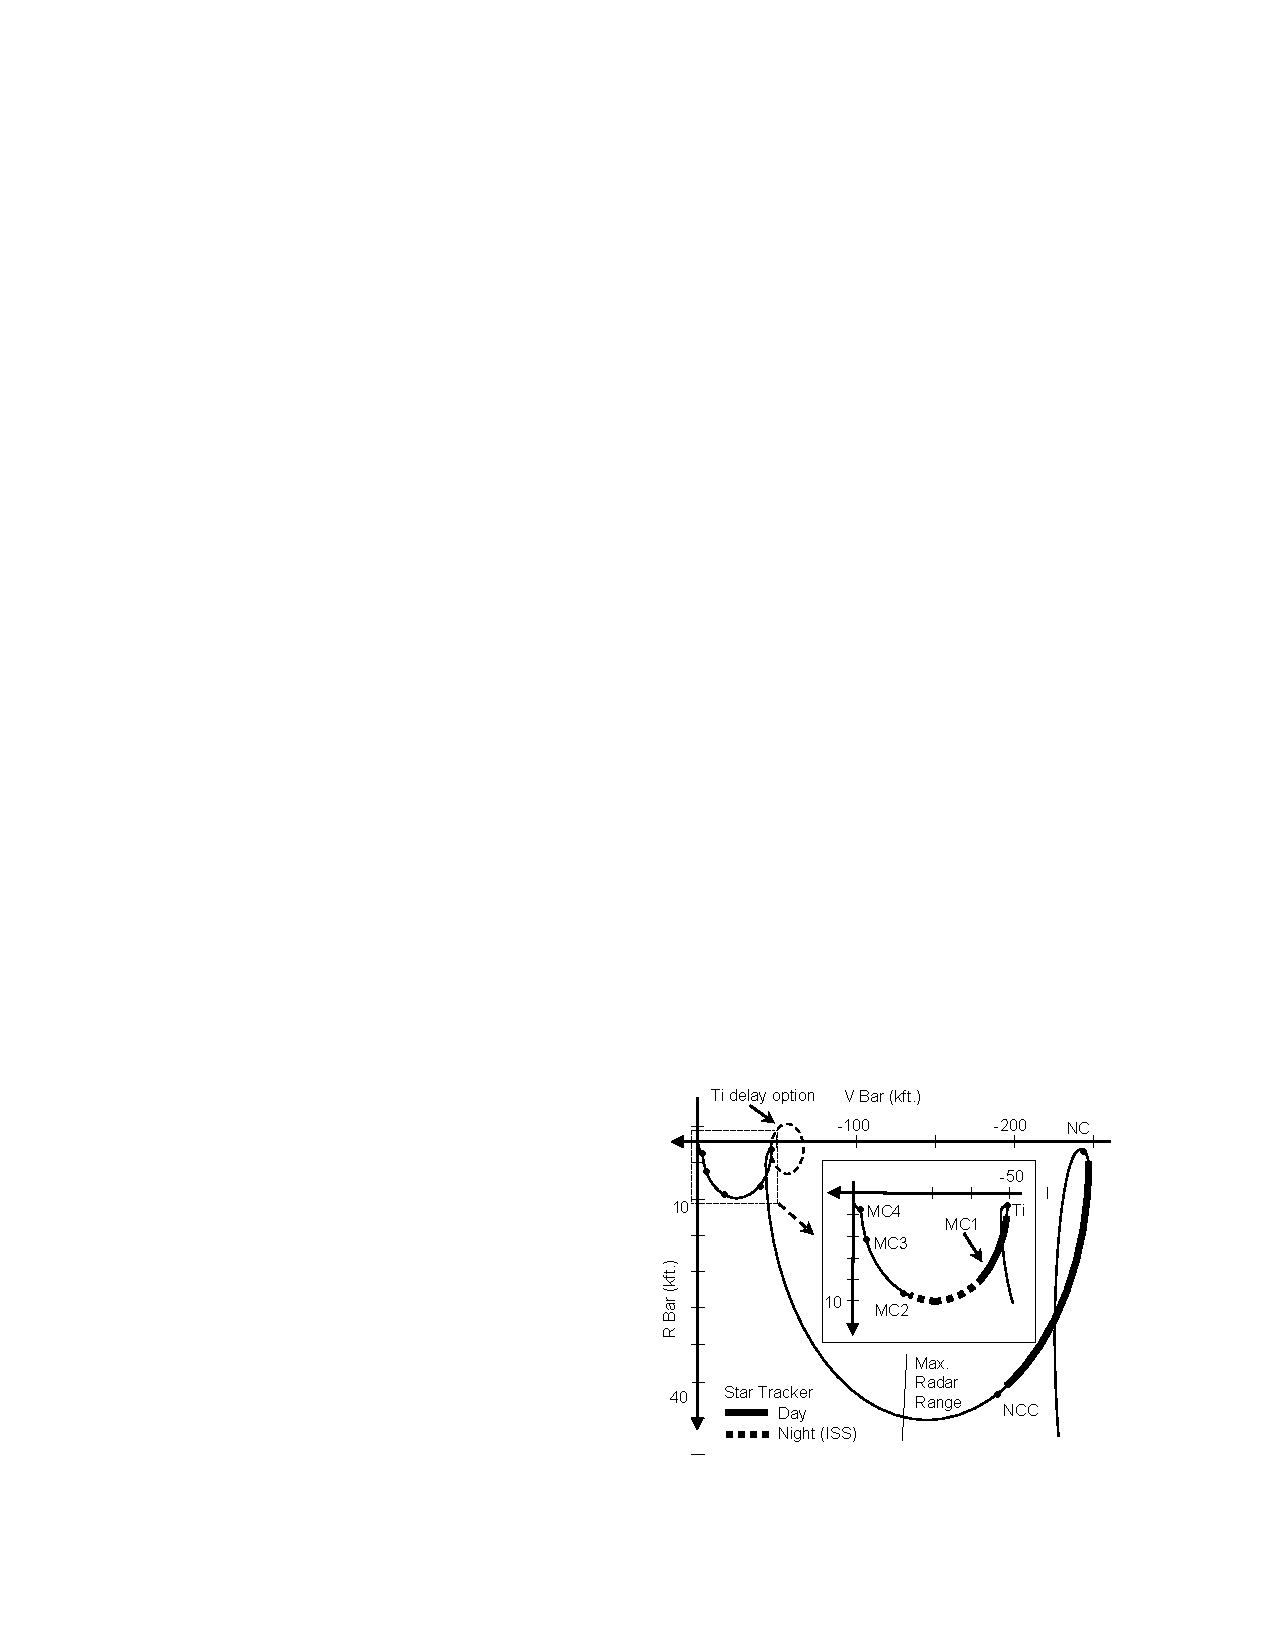
\includegraphics[width=.75\textwidth]{imgs/orbt.pdf}
\caption{Optimized R-Bar Targeted Rendezvous (ORBT) relative navigation rendezvous diagram.}
% \label{fig:density}
\end{center}
\end{figure}

Current orbital decay predictions place the Hubble Space Telescope (HST) at a nearly circular, 528 km altitude orbit during our proposed launch date of September 2019. After launch, HRV enters a 200 km, in-plane parking orbit, then enters a 500 km phasing orbit. From our phasing orbit, a homing maneuver bring the HRV to a holding point 15 km behind HST. When relative navigation sensors have acquired HST, the HRV will perform a closing maneuver to bring the final distance to 200 m below HST, after which an R-bar approach will be used to dock.

For the R-bar approach, our vehicle move up towards HST along its radial vector. Our vehicle will fire thrusters radially to close towards HST, and use small burns in the orbital velocity direction to negate the effects of orbital mechanics. If the R-bar is stopped at any point (in case of loss of communication or thruster failure, for instance), our vehicle will naturally move away from HST. During a jet fail scenario, the satellite will be guided away passively. During a jet fail on scenario, the satellite can would rotate to point the the failed thruster in such a way that it imparts $\Delta V$ away from HST. If, at any point in the docking, communication is lost, the HRV will automatically return to a holding point behind HST.

This approach has been adapted from the from the Space Shuttle's Optimized R-Bar Targeted Rendezvous (ORBT) profile~\cite{goodman2006history}. ORBT was developed to optimally set up initial conditions for a low energy coast up the +R-bar. This profile was used from 1997 to the end of Space Shuttle program in 2011, lending more than a decade of operational flight heritage.

\subsubsection{At what stage of the rendezvous are sensors active? Can we recover from a single sensor failure at each stage?}
\begin{table}[H]
\begin{center}
\begin{tabular}{l r r r}
\toprule
Sensor & \# Onboard & Upper Range & Lower Range \\
\midrule
Radar        & 2 & 100s of km & 100s of m  \\
LIDAR        & 2 & 10s of km & 2m  \\
Camera       & 2 & 100s of m & contact  \\
GPS          & 2 & - & -  \\
\bottomrule
\end{tabular}
\end{center}
\caption{Relative and absolute navigation sensors onboard the HRV.}
% \label{properties}
\end{table}

The most likely cause of failure for our spacecraft is a loss of attitude measurement. When the spacecraft is phasing with HST, its sources of attitude measurement are startrackers, a sun sensor, horizon sensors, and IMUs. Without frequent updates from the other attitude sensors, however, the IMUs experience drift and quickly become useless. Once the spacecraft comes within a few 10s of km of HST, however, radar and LIDAR can also be used calculate relative attitude. During final approach, the last few 100 m, stereo cameras can calculate sufficient pose estimation for docking.

There are at least two sensors available at all times for both attitude and navigation during all parts of the mission. During all phases of the mission, except for final rendezvous and docking, GPS navigation is sufficient to navigate. Once we begin the final stages of rendezvous and docking, there are three types of relative navigation sensors available. Two redundant radar sensors can be used to initially make relative navigations, and we can transition to LIDAR and optical measurements for the final 100s of meters. Horizon and sun sensors, and star trackers can be used for absolute attitude measurement for the early stages of the mission, and LIDAR and optical measurements can be used for relative pose navigation during the final stages of docking.

\subsubsection{How long can we stay at each part of the orbit?} \label{howlong}

If sufficient time has passed without contact with ground control, the HRV should automatically perform a deorbit burn. If additional failures, such a major electrical issue, prevent the HRV from deorbiting, there is a possibility of remaining in orbit for much longer than the intended mission duration.

Various orbital perturbations such as gravity gradients, solar pressure, magnetic field interactions, and atmospheric drag can decrease the altitude of the orbit. Of these factors, the largest for low Earth orbit is drag, which increases exponentially as the spacecraft lowers altitude. The force due to drag is
\begin{align*}
D &= \dfrac{1}{2} \rho v^2 A C_d
\end{align*}
in the direction opposite of the spacecraft's velocity. Here $\rho$ is the density of the atmosphere, $A$ is the cross-sectional area exposed to the atmosphere, and $C_D (\approx 2.2$) is the coefficient of drag. The solar radio flux can also change dramatically with the solar cycles, and has strong affects on the atmosphere. A program was developed under the assumptions of constant satellite mass, LVLH attitude, and $C_D$. $\rho$ is modeled as an exponential factor based on altitude.

There are three main circular orbits that the mission will take place in: 200 km orbit, 536 km orbit, and a 616 km orbit. As the satellite boosts itself (and Hubble) to higher, it expends fuel, which means that our satellite will always have a lower mass at higher orbits. The results and input parameters of the orbit lifetime analysis are listed in Table~\ref{altitude_table}. Satellites will remain in orbit longer at higher altitudes, where the atmospheric density is lowest. As such, the longest orbital lifetimes are at highest orbit, and the shortest lifetimes are at low altitudes. If satellite communication is not established within the first three days, the HRV will destructively re-enter the atmosphere.

% \begin{table}[H]
% \begin{center}
% \begin{tabular}{rrrrr}
% \toprule
% Altitude & 200km & 536km & 616km \\
% \midrule
% $m$ & 996 kg & 881 kg & 637 kg \\
% $t$ & 2.9 days & 99.5 years & 380 years \\
% \bottomrule
% \end{tabular}
% \end{center}
% \caption{$C_D$=2.2, $A=4$m$^2$}
% \label{altitude_table}
% \end{table}

\begin{table}[H]
\begin{center}
\begin{tabular}{lrrrrr}
\toprule
Mass (kg) &           600  &           700  &           800  &           900  &           1000 \\
Altitude (km)     &                &                &                &                &                \\
\midrule
100.0 &       0.3 &       0.3 &       0.4 &       0.4 &       0.4 \\
237.5 &      12.4 &      14.4 &      16.5 &      18.5 &      20.5 \\
375.0 &     544.7 &     635.4 &     726.1 &     816.8 &     907.5 \\
512.5 &   15073.3 &   17585.4 &   20097.5 &   22609.6 &   25121.7 \\
650.0 &  257994.8 &  300993.8 &  343992.8 &  386991.8 &  429990.8 \\
\bottomrule
\end{tabular}
\end{center}
\caption{Time to deorbit, in days with $C_D=2.2$, $A=4$ m$^2$.}
\label{altitude_table}
\end{table}

\subsection{HST Docking Interface} \label{lids}

\begin{figure}[H]
\begin{center}
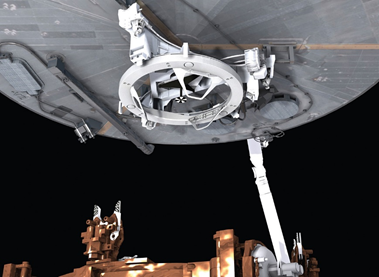
\includegraphics[width=.65\textwidth]{HST_Interface_Figures/H1A.png}
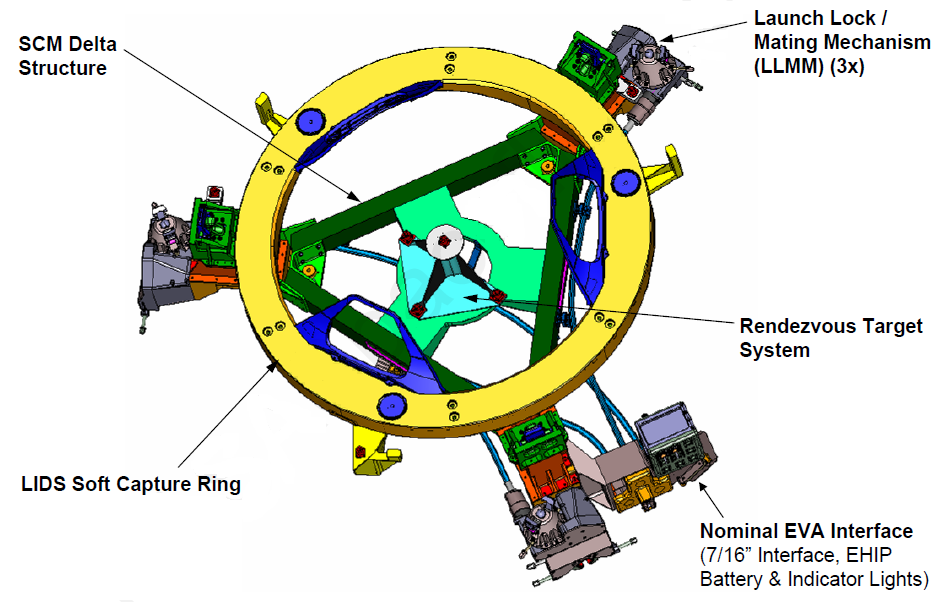
\includegraphics[width=.65\textwidth]{HST_Interface_Figures/H1B.png}
\caption{Hubble's Soft Capture Mechanism (SCM).}
\label{H1}
\end{center}
\end{figure}
The HST soft-capture mechanism (SCM) was installed in phase 1 of service mission 4 in order to enable future rendezvous missions and reduce design complexities~\cite{ref1}. The SCM is the white-ring structure shown attached to the aft of the HST in Figure~\ref{H1}a. In Figure~\ref{H1}b, the SCM is isolated where the ring is 1.83 m (72 inches) in diameter and the total structure height is 0.61 m (2 feet).

The docking system utilizes a Low Impact Docking System (LIDS) and contains targets to aid capture and docking operations. The LIDS design is part of an ongoing effort to develop a ``reconfigurable, active, closed-loop, force-feedback controlled docking system that is standardized''~\cite{ref3}. One of the greatest benefits of the system is that it is androgynous; that is, two copies of the same design can dock together. Therefore, design complexity and, subsequently, developmental and time costs are reduced when the HRV employs the same LIDS design. As an added benefit of the LIDS system, the HST capture envelope has significantly improved. The capture limits of the docking mechanism, as shown in Table~\ref{table:capture_limits}, will allow for easier rendezvous and docking when using the LIDS system on the HRV. Using this information, requirement (b) from Section~\ref{section:reqs} will be fulfilled.

\begin{table}[H]
\begin{center}
\begin{tabular}{l r r}
\toprule
Limit Parameter & Limit & Rate Limit \\
\midrule
Lateral & 11.4 cm & 1.3 cm/s \\
Range & 20.3 cm & 5.1 cm/s \\
Roll & 4 degrees & 1 degree/s \\
Pitch & 4 degrees & 0.25 degrees/s \\
Yaw & 4 degrees & 0.25 degrees/s \\
\bottomrule
\end{tabular}
\end{center}
\caption{Capture Limits of the SCM.}
\label{table:capture_limits}
\end{table}

\begin{figure}[H]
\begin{center}
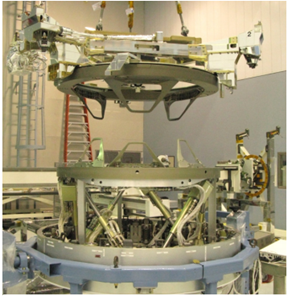
\includegraphics[height=0.4\textheight]{HST_Interface_Figures/H2.png}
\caption{SCM Demonstration.}
\label{H2}
\end{center}
\end{figure}

The HRV interface is defined to be in full contact when the active system latches are fully engaged with the passive latch strikers~\cite{ref5}. The system on the HST is a passive system; therefore, the reboost vehicle's docking system must actively adjust itself to meet the clearances placed by Table~\ref{table:capture_limits}. After the boosting phase of the mission has been completed, the active system must have actively loaded springs that will propel it away from the HST for safe deorbiting. In doing so, requirement (e) from Section~\ref{section:reqs} will be fulfilled.


%----------------------------------------------------------------------------------------
%	Electronics
%----------------------------------------------------------------------------------------

\section{Electronics}

The electronics subsystem contains the four main components necessary for operation. A Command and Data Handling (C\&DH) board is used for the majority of computations. Solar panels are used to collect solar energy. Battery cells are used to store energy until needed. An Electrical Power Subsystem (EPS) board regulates the power regulation and distribution through the satellite.

Although the HRV mission will not take it to altitudes above 650km, radiation can still be a concern. Above a portion of the magnetosphere, the HRV is not as protected as electronics on the ground. Alpha, Beta, and Gamma radiation can cause errors within data storage and data processors. The inner Van Allen belts start around 700km or higher over most parts of the Earth. This means that the first layer of heavy particles should start well above the operational altitude of the HRV. However in locations such as the South Atlantic Anomaly, the radiation can dip to far lower altitudes and is highly unpredictable. Because of the importance of the reboost target, the radiation environment is exaggerated to ensure proper operation of the spacecraft and the ability to recover from single event upsets. Three processors and three memory storage devices will allow comparisons for all signals in order to determine faulty data caused by upsets.

The EPS board is required to ensure proper power to all components as well as regulate battery charging. This is the hub where the power bus, solar panels, and battery cells come together. The EPS board is in charge of both operation and safety of the power system.

The batteries will have internal charging circuits. These charging circuits are not software dependent and much more reliable. This internal circuit uses the battery voltage to determine the depth of discharge (DoD) of the cell. The onboard circuit will prevent possible dangers due to overcharging. However, since it is a physical circuit, the DoD required to start charging the batter cannot be changed internally. Though it cannot be changed on the internal circuit, the EPS board can be used to manipulate the system into charging early if necessary by opening up a very large resister in line with the battery. This drops the circuit voltage which makes the internal sensor think the DoD has dropped below charging threshold.

The batteries will be Lithium Nickel Manganese Cobalt Oxide (NMC) Cells. Lithium Ion cells have a high energy density and NMC cells are safer relative to some other Lithium Ion cells. The only drawback is a slightly lower energy density but since we are not near the maximum launch weight for our vehicle, the additional safety is worth the additional mass. NMC batteries can achieve 150 Wh/kg.

The solar panels will be flush mounted on all sides except the fore and aft endplates. They will cover the entirety of the sides with the exception of small thermal radiator panels. For analysis purposes, a solar panel efficiency of 30\% was used.

To perform a power budget analysis all consumptions must be accounted for. There are only a couple of phases that use more power than just system overhead. At any given time the system must be monitoring its own health, position, and attitude. Major burns require enough power to actuate the engine valve. The entire rendezvous phase has increased power usage. Beyond these factors the only other large consumption is during large data transfers. Small effects are also included such as battery heating and solar inefficiencies.

Power generation was estimated using eclipse times generated using Systems Tool Kit (STK), average area to the sun, and average power available at Earth. The power available is a constant estimate for the duration of the mission. The eclipse duration is dependent on the altitude and the average area to the sun depends on what phase of the mission the HRV is on. The DoD a cell will reach is also dependent on the phase of the mission. During early phases of the mission the batteries are allowed to fall to a lower charge level to reduce the charge cycles performed. Right before and during mission critical phases, the batteries are not allowed to drop as low.

Due to the inability freely point while attached to HST, power generation will be assumed to be zero for this portion of the mission. With all power generation and consumption properly simulated, the capacity of the batteries is modified until the maximum desired DoD is not exceeded. As you can see from the results presented in Figure~\ref{fig:battery}, a battery capacity of 600 Wh is sufficient. This would be a mass of less than 3.5 kg for the primary cell and an additional 3.5 kg for the backup cell. With this battery cell the maximum depth of discharge brings the batter capacity down to 52\%, but only during the rendezvous phase. Other than that specific portion of the mission, the battery capacity doesn't go below 75\% of maximum capacity.

\begin{figure}[H]
\begin{center}
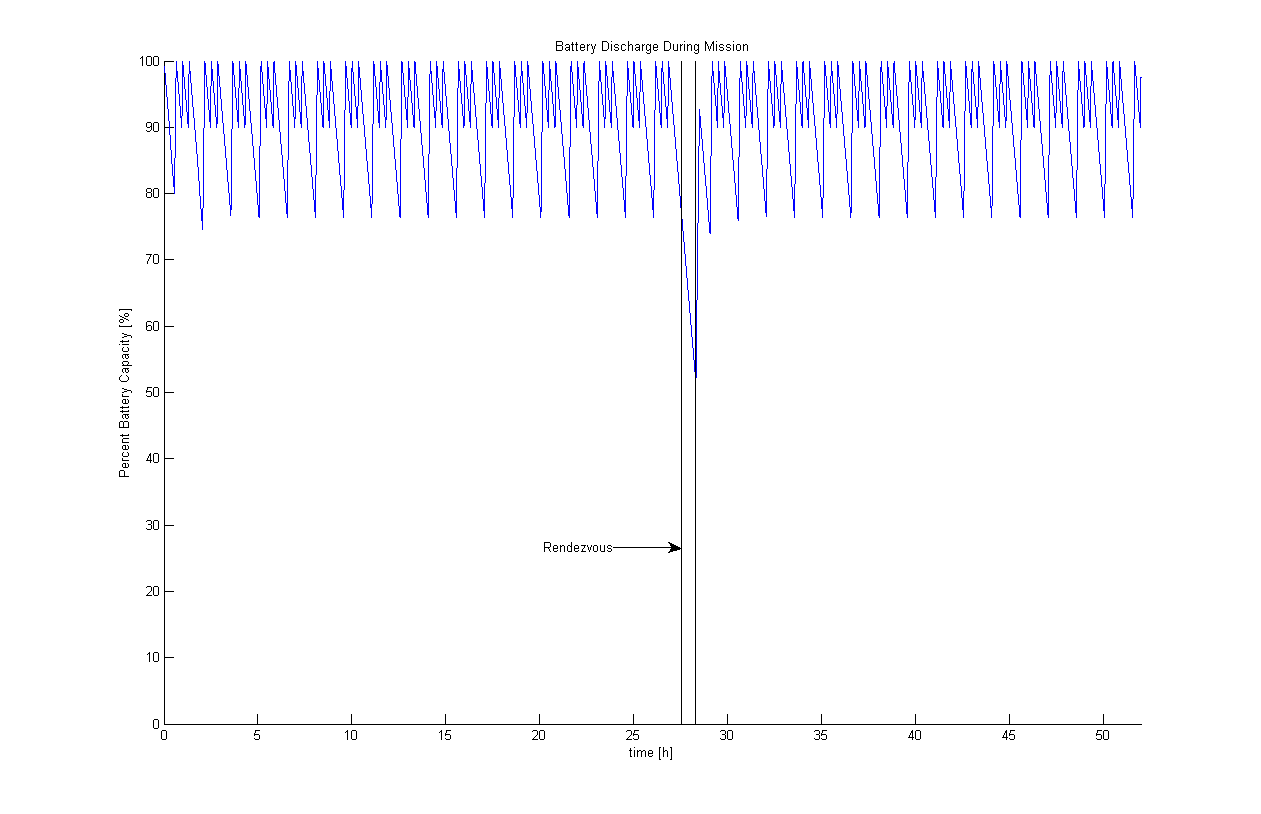
\includegraphics[width=.8\textwidth]{figs/BatteryDischarge.png}
\caption{Battery capacity for duration of mission.}
\label{fig:battery}
\end{center}
\end{figure}

\begin{table}[H]
\begin{center}
\begin{tabular}{l r}
\toprule
System & Value \\
\midrule
Solar Panel Area		& 16 m$^2$	 \\
Solar Panel Efficiency	&  0.3	 \\
Orbit Average Power		&  975W	 \\
Battery Capacity		& 600Wh	 \\
Battery Mass			& 3.5kg	 \\
Maximum DoD				&  48\%	 \\
\bottomrule
\end{tabular}
\end{center}
\caption{Summary of Power System.}
% \label{properties}
\end{table}

%----------------------------------------------------------------------------------------
%	Communications
%----------------------------------------------------------------------------------------

\section{Communications}

HST has two low gain and two high gain s-band antennae~\cite{csm}. The two low gain antennae (LGA) are mounted fore and aft providing two 95\% spheres of coverage with very little blackout areas. The two high gain antennae (HGA) are mounted on either side extended on booms. The LGA can transmit or receive to TDRSS, a ground station, or an orbiter, while the HGA can only transmit through TDRSS. For this reason the HRV shall have an s-band antenna capable of communicating with HST through the LGA.

The HRV will be able to send up to 1000 bps of command and ranging information at 2106.4 MHz to HST while receiving up to 32 kbps of engineering data at 2287.5 MHz from HST. These are the same frequencies whether data is relayed through TDRSS or not. If HRV is communicating with the ground station, these bitrates increase to 192 kbps downlink and 72 kbps uplink~\cite{usa2010european}. The HRV can communicate through TDRSS or directly to the ground station. TDRSS allows for continuous coverage therefore it will be the choice for mission critical operations.

S-band also provides robustness. S-band can penetrate dense clouds with less energy loss. S-band also has a longer wavelength; the wider beam makes it easier to lock onto another antenna. The only main drawback is the bitrate, but the bitrate is acceptable for our application.

In order to ensure continuous communication with HST during rendezvous, a similar fore and aft LGA configuration will be used. The layout was designed to ensure HST had the widest possible antennae coverage which is the same goal of the HRV LGA antenna. While each HST LGA is 20W, each HRV LGA will be slightly higher at 25W each for ease of acquisition by receiving antennae. Each HRV HGA will be 20W while each HST HGA is only 15W.

In order to send larger data dumps and telemetry during different parts of the mission a 25W Ku-band antenna will also be included. It is not capable of communicating with HST but can be used to transmit at higher bitrates directly to ground control or through TDRSS. Ku-band is a higher bitrate but more susceptible to bad weather and is harder to lock onto therefore will not be used solely for mission critical operations. It will however be used as a supplemental parallel data transfer. It will use 13.755 GHz to receive and 15.003 GHz to transmit to TDRSS. At up to 50 Mbps, much larger transfers can be performed in short amounts of time.

\begin{table}[H]
\begin{center}
\begin{tabular}{l l r r r r r}
\toprule
Band & Gain & Tx Freq & Rx Freq & Tx Rate & Rx Rate & Power  \\
\midrule
S (2) & Low & 2106.4 MHz & 2287.5 MHz & 1000 bps & 32 kbps & 25 W \\
S (2) & High & 2106.4 MHz & 2287.5 MHz & 72 kbps & 192 kbps & 20 W \\
Ku & NA & 13.755 GHz & 15.003 GHz & 50 Mbps & 50 Mbps & 25 W \\

\bottomrule
\end{tabular}
\end{center}
\caption{Antenna Summary.}
% \label{properties}
\end{table}

\begin{figure}[H]
\begin{center}
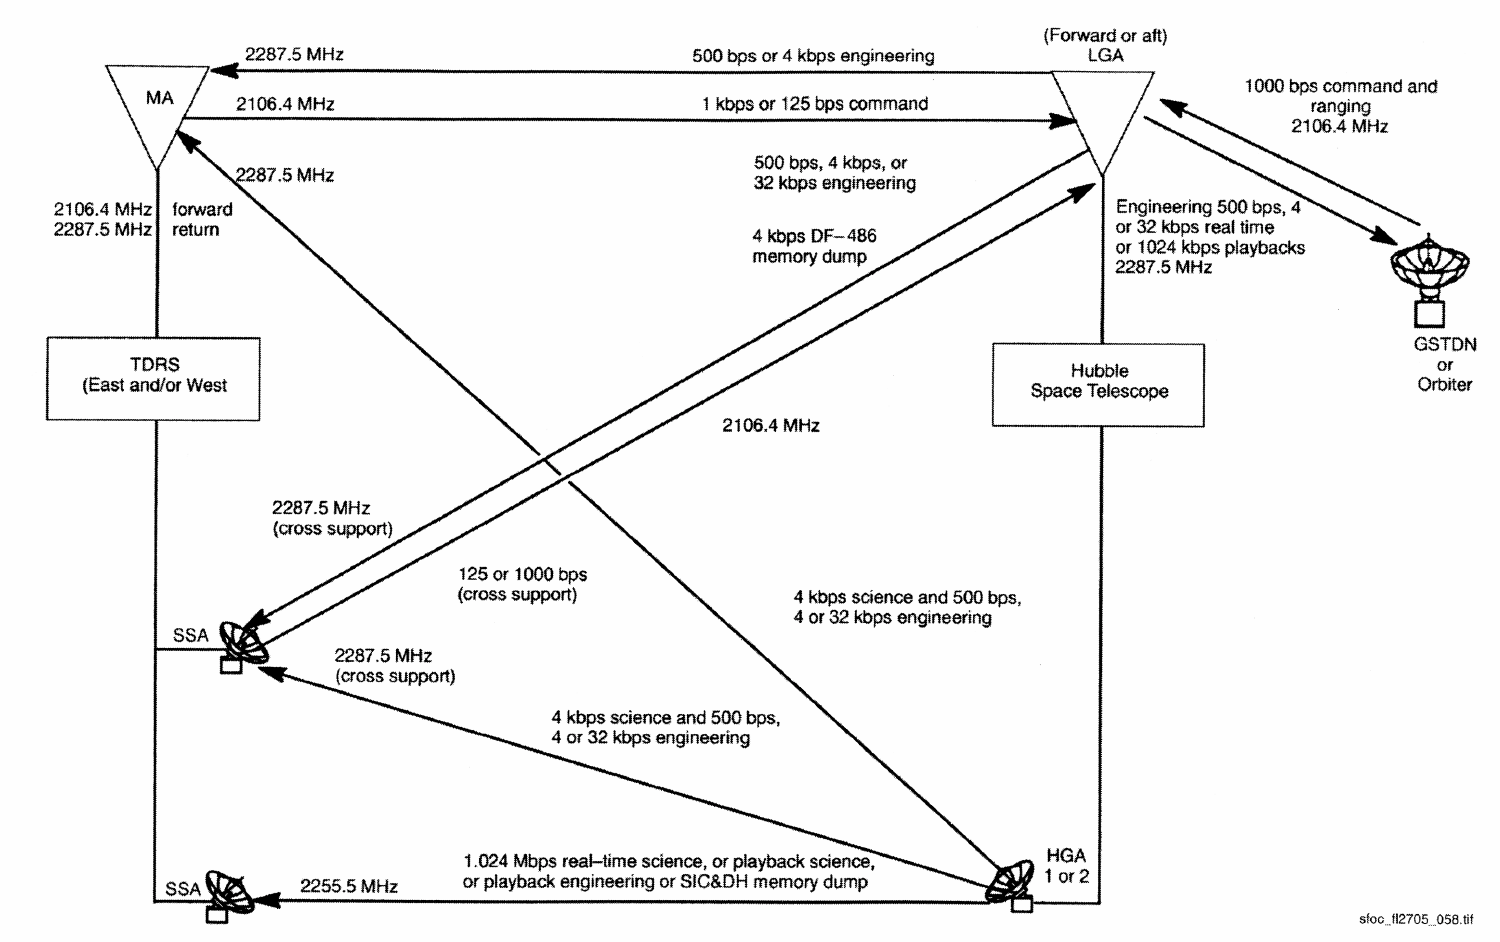
\includegraphics[width=1\textwidth]{figs/HSTcom.PNG}
\caption{HST communication.}
% \label{fig:density}
\end{center}
\end{figure}


%----------------------------------------------------------------------------------------
%	Thermal
%----------------------------------------------------------------------------------------

\section{Thermal}

There are a few sources of heat that need to be dissipated. The system bus and communications consume power while even on standby mode which generates heat. The solar panels are also large sources of heat while they are exposed to the sun, but the power they produce is not being dissipated into batteries. This means anytime the HRV is not charging its batteries and not in eclipse, it is producing a fair amount of heat that needs to be expelled. One source of heat but not as significant is radiative heating from the plume behind the craft every time a burn is performed.

External thermal radiator panels will be used to dissipate heat from the craft. Surfaces are also specially selected to balance the emissivity and absorbance of radiative energy between different components. Various heat pipes and silicon pads are strategically placed in order to direct the heat flow properly.


%----------------------------------------------------------------------------------------
%	ADCS
%----------------------------------------------------------------------------------------

\section{ADCS}
\subsection {Overview}
The attitude determination and control system (ADCS) uses sensors to find the attitude information of a spacecraft and compute control torques for pointing requirements and stabilization. The overview of the ADCS components are illustrated in the block diagram below.
\begin{figure}[H]
\centering
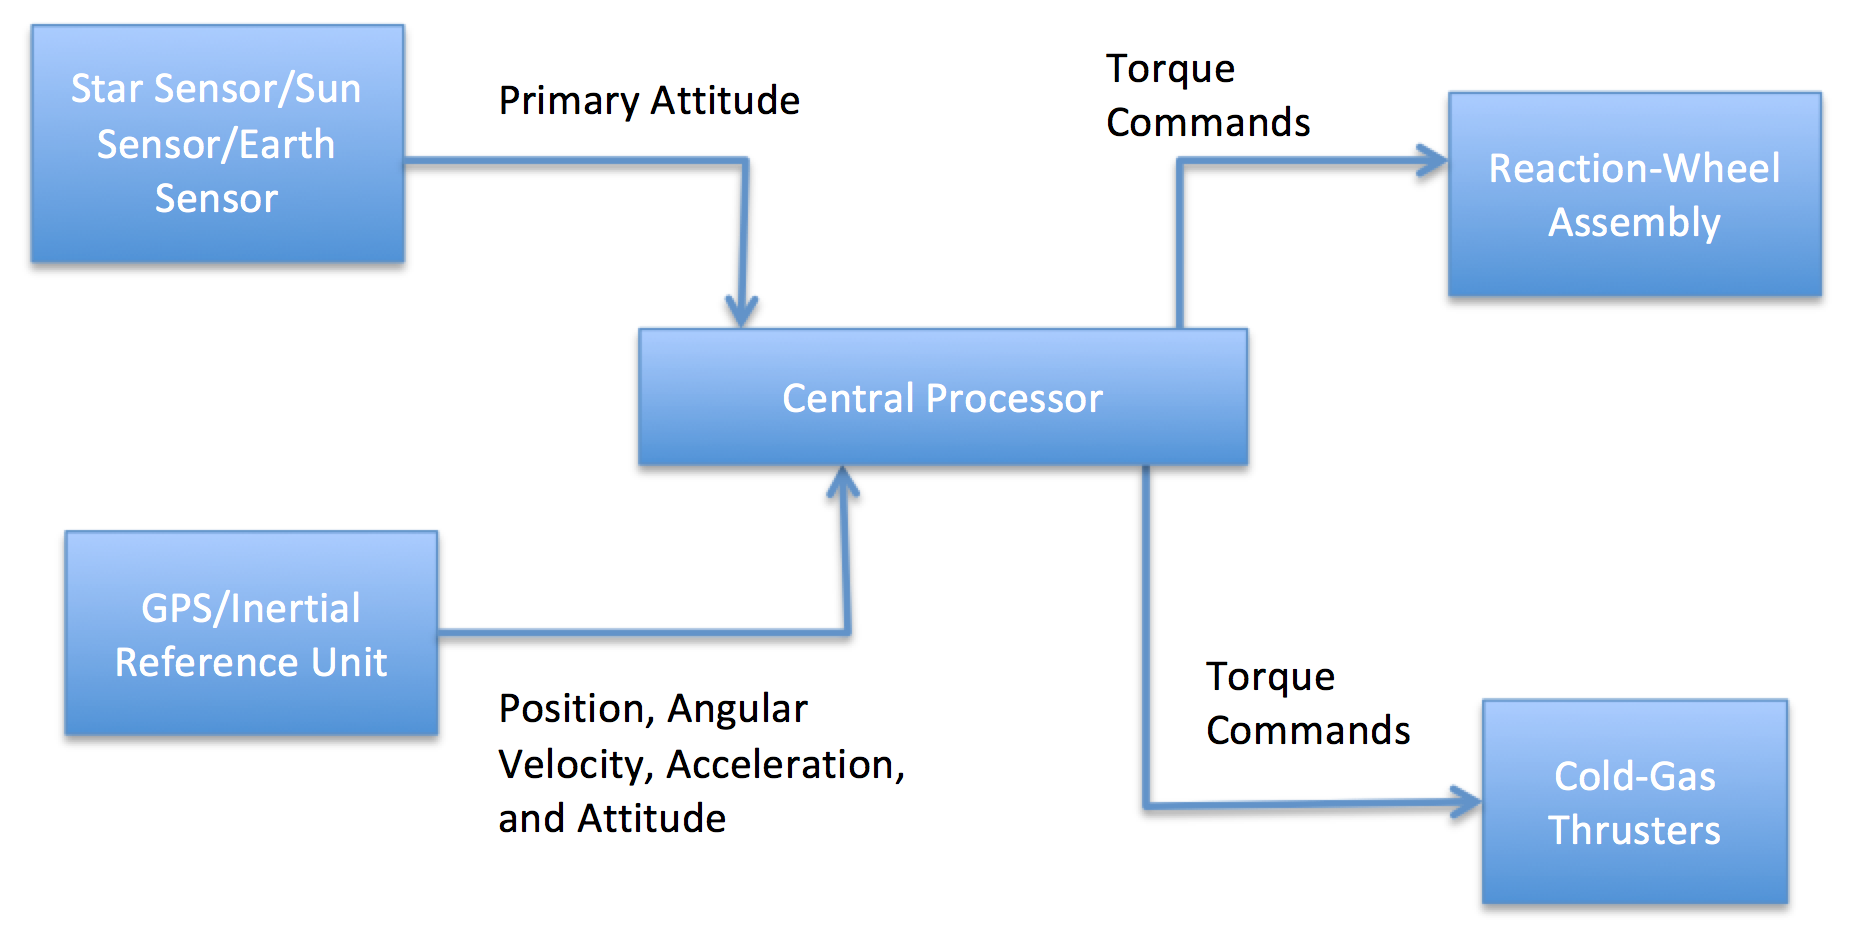
\includegraphics[width=1\textwidth]{GNCHardware.png}
\label{fig:adcs}
\caption{Overview of Attitude Determination and Control System.}
\end{figure}


\subsection{Determination of Control Modes}
The ADCS is expected to execute several control modes throughout the various mission phases. The mission requirements drive these control modes.
\begin{enumerate}
\item Orbit Insertion Mode
\par During this phase, the HRV is launched to its parking orbit, and the ADCS performs no control maneuvers until the vehicle has completely separated from the launch vehicle, and has reached its initial orbit.
\item Acquisition Mode
\par The spacecraft determines its initial attitude and stabilization parameters immediately after launch. This phase is crucial for communicating with ground control and obtaining information to generate power. The sun and earth sensors are switched on, and satellite-attitude data computed by the central processor is sent to ground control. The HRV subsequently transitions into the Sun Acquisition Modes, in which the vehicle is oriented toward the sun for power generation. The sun sensors allow the vehicle to lock onto the sun and maintain its attitude, as the solar arrays are deployed. Following the sun-pointing maneuver, the vehicle undergoes an additional maneuver in the Earth Acquisition Mode to approach a nadir-pointing attitude for the earth sensors.
    \begin{enumerate}
    \item Sun Acquisition Mode
    \item Earth Acquisition Mode
    \end{enumerate}
\item Normal Mode
\par In this phase, the attitude of the spacecraft stays inertially fixed. The ADCS will monitor spacecraft attitude and send attitude information to the ground station.
\item Slew Mode
\par ADCS counters torques arising from external disturbances and performs momentum unloading. Further, the spacecraft attitude is maintained in its sun- and nadir-pointing attitude.
\item Safe Mode
\par The ADCS needs to account for emergencies in which regular mode fails or is disabled. In this phase, all non-essential equipment and actuators are switched off. When the vehicle recovers, the ADCS transitions to the Sun Acquisition Mode and reorients the vehicle to the optimal sun-pointing attitude.
\end{enumerate}

\bigskip Table~\ref{table:scctrl} summarizes the ADCS equipment associated with the control modes.

\begin{table}[H]
\centering
\begin{tabular}{l l l}
\toprule
Mode & Sensors & Actuators \\
\midrule
Orbit Insertion & None & None \\
Acquisition  & Sun and earth sensors & Reaction wheels \\
Sun Acquisition & Sun sensors & Reaction wheels\\
Earth Acquisition & Earth and sun sensors & Reaction wheels \\
Normal & Earth, sun, and star sensors, GPS & Reaction wheels, cold gas thrusters \\
Slew & Star sensors & Reaction wheels, cold gas thrusters  \\
Safe & Sun and earth sensors & Reaction wheels \\
\bottomrule
\end{tabular}
\caption{ADCS Equipment Associated with Control Modes.}
\label{table:scctrl}
\end{table}

\subsection{Quantification of Disturbance Environment}
\par Torques can arise from external and internal disturbances. External disturbances are influences of the environment, such as aerodynamic drag and gravity gradient. In contrast, internal disturbances arise from the spacecraft itself.

\subsubsection {External Disturbance Torques}
\par The following environmental disturbances will affect the HRV
\begin{enumerate}
\item Aerodynamic drag
\item Magnetic field
\item Gravity gradient
\end{enumerate}

\bigskip \par Aerodynamic drag induces torques, and the amount of torque caused by aerodynamic drag depends on the spacecraft geometry, attitude, and altitude. In addition, disturbance torques due to the gravity gradient and magnetic field are significant for altitudes below 500 km.

\bigskip \noindent The torque given by atmospheric drag is
\begin{equation*}
T_a = \frac{1}{2}\rho C_d A_r V^{2}(cp_a - cm)
\label{equation:ta}
\end{equation*}
where $\rho$ is the atmospheric density, $C_d$ is the total drag coefficient, $A_r$ is the profile area of the satellite in the direction of motion, $V$ is the velocity of the spacecraft, $cp_a$ is the center of aerodynamic pressure, and $cm$ is the center of mass. In general, the atmospheric density varies with time of day and level of solar activity.

\noindent The magnetic field gives a torque of
\begin{equation*}
T_m = D\left(\frac{M}{R^{3}}\lambda\right)
\label{equation:tm}
\end{equation*}
where $M$ is the sum of all magnetic moments in the spacecraft and $B$ is the geomagnetic field vector.

\noindent The gravity gradient induces a torque of
\begin{equation*}
T_g = \frac{3\mu}{2R^{3}} | I_z - I_y | sin(2\theta)
\label{equation:tg}
\end{equation*}
where $\mu$ is Earth's gravitational constant $(3.986 \times 10^{14} \mathrm{m^{3}/s^{2}})$, $R$ is the distance from the center of Earth, $I_z$ and $I_y$ are the moment of inertia about the Y and Z axes, and $\theta$ is the angle between the local vertical and the Z principal axes.

\subsubsection{Internal Disturbance Torques}
Torques may arise from the internal components within a spacecraft. Moving parts, such as rotating wheels and fuel sloshing, can induce torque on the spacecraft, as well as an actuator misalignment with the center of gravity. The following internal disturbances were concerned for the ADCS system of the HRV

\begin{enumerate}
\item Rotating wheels (reaction wheels)
\item Thruster misalignment
\end{enumerate}

\bigskip
\par Rotating wheels cause torques that affect the stability of the vehicle and accuracy of the ADCS measurements. Misalignment of thrusters also creates unbalanced torques when they are in use.

\subsection{Selection of Spacecraft-control Types}
The following attitude-control modes were selected for the ADCS of the HRV
\begin{enumerate}
\item Zero momentum (thrusters)
\item Zero momentum (three-wheel)
\end{enumerate}

\par Both the zero momentum thruster and three-wheel systems were selected because they can provide any combination of slew maneuvers in the pitch, roll, and yaw directions, and have no pointing constraints. In addition, these control methods allow for high maneuverability rates, which is an advantageous for the short-duration mission. Generally, some drawbacks to these control techniques are the limited lifespan due to the dependency on propellant, sensors, and wheels; and the higher costs and complexity. For the reboost mission, the limited lifespan does not play a major role in the mission outcome because the entire mission will be completed in no more than a single week. Further, the vehicle will approach and dock with the Hubble Space Telescope, which merits additional costs and complexity.

\subsection{Selection and Sizing of ADCS Hardware}
\begin{table}[H]
\begin{center}
\begin{tabular}{l r r}
\toprule
Sensor & \# Onboard & Performance \\
\midrule
Horizon Sensor~\cite{earth_sensor} & 2 & 0.25 deg \\
Sun Sensor~\cite{sun_sensor}     & 1 & 0.1 deg \\
Star Tracker~\cite{star_tracker}   & 2 & 2.8 arcsec \\
GPS/IMU~\cite{gps_ins}        & 2 & 0.01 deg/hr \\
\bottomrule
\end{tabular}
\end{center}
\caption{Attitude measurement sensors onboard the HRV.}
% \label{properties}
\end{table}

\subsubsection{Sensors}
\noindent Multiple sensors needed to be selected to obtain a complete three-axis attitude measurement, as certain sensors gave only two angles of attitude data. The ADCS needed to have sensors that could provide a high degree of accuracy because the vehicle was planned to dock with the \$2.5-billion HST. The following sensors were selected for the HRV
\begin{enumerate}
\item NewSpace Systems Fine (Digital) Sun Sensor
\item Maryland Aerospace Static Earth Sensor
\item Sodern HYDRA CMOS Star Tracker
\item Honeywell Enhanced Space Integrated GPS/INS
\end{enumerate}
\bigskip
\par Sun and horizon sensors were selected because they provide accurate measurements of the spacecraft attitude, and together complete the required three-axis attitude data set. For eclipse periods in which the sun sensors could not provide data, GPS and inertial navigation sensors were included in the ADCS. Finally, star sensors were included because they give the most accurate attitude measurements and all three Euler angles. In brief, the collection of these sensors will provide continuous measurements of spacecraft attitude with a high level of accuracy.
\subsubsection{Actuators}
The attitude measurements are sent to the central processor, which computes a control torque for stabilization and pointing requirements. The vehicle needed to attain maximum capacity with the solar arrays throughout the mission; therefore, continuous range of torque was a significant driver in the ADCS design. To adjust the attitude of the spacecraft, control torques are applied to the spacecraft by use of actuators. The following actuators (and quantities) were selected for the ADCS
\begin{enumerate}
\item Cold gas thrusters (12)
\item Reaction wheels (4)
\end{enumerate}

\par Reaction wheels were selected because they are light weight and can produce a continuous range of torque, fulfilling the pointing and mass requirements. Additionally, cold gas thrusters were selected for momentum dumping, performing the rendezvous with the HST, and additional orbital maneuvers. Compared to other actuators, they offer many advantages: they have a relatively simple design, offer safe operating conditions, and have been established since the 1960's.

\begin{table}[htb]
\centering
\begin{tabular}{l r l r}
\toprule
Vendor & Thrust (N) & Propellant & Dry mass (g)\\
\midrule
VACCO~\cite{cold_gas_thruster}              & 8.9 	& Nitrogen      &  376 \\
Marotta Cold Gas Microthruster~\cite{cold_gas2} & 2.2 	& Nitrogen	& 70 	\\
Moog 58-103~\cite{space_props}				& 5.55	& Nitrogen	& 15 	\\
\bottomrule
\end{tabular}
\caption{Cold Gas Thrusters Available Options.}
\label{table:cgta}
\end{table}

\par Listed in Table \ref{table:cgta}, several options were available for the cold gas thrusters. The VACCO thrusters were selected because they offered the highest thrust. Although they were the heaviest of the considered thrusters, the mass budget allowed for the additional weight.

\par To size the reaction wheels, a saturated angular velocity and time to reach saturation were assumed for each wheel
\begin{equation*}
\alpha_w t = \omega_{sat}
\label{equation:alphasat}
\end{equation*}
where $\alpha_w$ was the angular acceleration of the rotating wheel, $t$ was the time to reach saturation, and $\omega_{sat}$ is the angular velocity of the rotating wheel at saturation. The time to saturation was assumed to be the duration of the mission of 60 hours, and the angular velocity at saturation was arbitrarily estimated.

In addition, the torque produced by the rotating wheel depended on the moment of inertia of the wheel, and its angular acceleration

\begin{equation*}
T_p = I_w \alpha_w
\label{equation:tp}
\end{equation*}

The moment of inertia of a wheel was given by
\begin{equation*}
I_w = \frac{1}{2}MR^{2}=\frac{1}{2} \rho_{w} \pi R_{w}^{4} t_{w}
\label{equation:iw}
\end{equation*}
where $\rho_{w}, R_{w},$ and $t_{w}$ were the material density, radius, and thickness of the wheel, respectively. To compensate for frictional loss, the torque produced by the wheel was a percent increase arbitrarily selected from the torque required by the wheel. Numerical iteration was performed to determine the wheel radius and thickness that would ensure compliance with mass and volume constraints.

\begin{table}[H]
\centering
\begin{tabular}{l r}
\toprule
Characteristic & Value\\
\midrule
Number & 4 \\
Radius & 5.9 in \\
Thickness & 0.67 in \\
Mass $(\times 4)$ & 13.5 kg \\
Angular momentum & 29.9 \textup{kg} $\cdot$ \textup{m}$^{2}$\textup{/s}  \\
\bottomrule
\end{tabular}
\caption{Reaction Wheel Specifications.}
\label{table:actspecs}
\end{table}

\begin{table}[H]
\centering
\begin{tabular}{l r l r}
\toprule
Vendor & Thrust (N) & Propellant & Dry mass (g)\\
\midrule
VACCO                                     & 8.9     & Nitrogen      &  376 \\
Marotta Cold Gas Microthruster & 2.2    & Nitrogen  & 70    \\
Moog 58-103             & 5.55  & Nitrogen  & 15    \\
\bottomrule
\end{tabular}
\caption{Cold Gas Thrusters Available Options.}
\label{table:actspecs}
\end{table}

Table \ref{table:actspecs} summarizes the specifications of the reaction-wheel assembly. With the combination of the reaction wheels and cold gas thrusters, the ADCS actuators will ensure optimal power generation and a successful rendezvous with the HST.

\subsection{Definition of Algorithms for Determination and Control}

The ADCS operates as a feedback control system, based on an exchange of information among the central processor, sensors, and actuators. The sensors provide information to the central processor on the spacecraft position, attitude, translational and angular velocities, and angular acceleration. The processor subsequently uses algorithms to compute a new vehicle attitude, angular velocity, and angular acceleration that maintain a nadir- and sun-pointing attitude, and minimize control torques. Following these computations, control commands are sent to the ADCS actuators to perform the proper attitude adjustments.

\begin{enumerate}
\item[$\bullet$] Determination: Parameterized as sequential rotations about the axes of a reference frame (Euler angles)
\item[$\bullet$] Control: 3-axis PD controller, calculate error angle for each axis, and resulting control torque
\end{enumerate}

\subsection{Test Plan}
The ADCS can be tested on the 3 DoF Granite Lab at NASA Ames Research Center. This table was machined to be ultra flat, and serves as an air-bearing table with CO2 gas coming from the bottom of the table, allowing the ADCS to essentially float. On this surface, the ADCS can be tested in the X and Y rotation directions. External disturbances may be additionally simulated by having a stream of air pointed at the ADCS, and corresponding control torques can be applied to the system. Measurements should subsequently be made on the accuracy of the attitude adjustments.

\subsection{Conclusion}
The ADCS takes attitude information from sun sensors, earth sensors, star trackers, and an integrated GPS/INU system. Continuous data will be fed into the central processor to a high degree of accuracy, and control torques will be computed and sent to the cold gas thrusters and reaction wheels. The control commands will fulfill the pointing requirements, maintain spacecraft stabilization, and provide safe operating conditions during the rendezvous with the HST. In sum, the ADCS satisfies the system requirements and will help the HRV achieve mission success.

%----------------------------------------------------------------------------------------
%	Launch Vehicle
%----------------------------------------------------------------------------------------

\section{Launch Vehicle}

Customer requirement (a) from Section~\ref{section:reqs} is fulfilled by not considering international vehicles such as the Chinese Long March and the Russian Proton. In addition new vehicles expected to launch in 2016, such as the Minotaur C and Vulcan will also not be considered due to a lack of flight history.

\subsection{Design Drivers}

Before all other concerns are considered, the primary requirement for the launch vehicle is the capability to carry our payload to a desired orbit. As seen in Section~\ref{section:structure}, the final design's mass is estimated to be 1098 kg. Additionally, per requirement (a), the launch vehicle must take-off from Cape Canaveral into a 28.5 degree orbital inclination.

The HRV must also fit inside the launcher's payload fairing. The size of the reboost vehicle is, as mentioned in Section~\ref{section:structure}, dependent on the SCM and the propellant mass. The SCM has an outer diameter of 1.83 m (72 inches), which drives the square block to have a diagonal dimension of 2.57 m (101.8 inches). The length of the HRV bus is found to be 2.2 meters (86.6 inches) after the placement of necessary sensors and other subsystems. Adding the length of the docking mechanism, and the nozzle, the total length of the spacecraft is approximately 3.42 meters (134.6 inches).

In addition, the insertion accuracy of the vehicle must be adequate in order to not incur heavy mass and time costs. An accuracy on the order of 100 km, for example, is indefensible since the payload will be either heavier or lighter than expected. For example, if the HRV is inserted 100 km above the target, then the spacecraft has extra fuel it must expend. In addition, the rendezvous plan must be redrawn and an additional measure to burn-up the extra fuel before deorbit must be made. In the worst case scenario, the spacecraft is inserted into an orbit below the target parking orbit and must now face higher than expected drag forces. The spacecraft would then expend enough fuel to reach the HST yet with an inadequate amount for mission completion. Therefore, in order to ensure acceptable orbital insertion accuracy, vehicles with liquid propellant final stages will be required since they are controllable.


\subsection{Vehicle Parameters Tabulated}
The payload capacity of each vehicle of interest is tabulated along with their serviceability status at Cape Canaveral. The largest vehicles have GEO launch capabilities while the smallest can only send 450 kg of payload to a 200 km orbit. The Antares launcher is removed from consideration since it hasn't been serviced at Cape Canaveral, while the Pegasus and Minotaur I are removed due to their minimal payload capacities.

\begin{table}[H]
\centering
\begin{tabular}{l l l}
\toprule
Vehicle &  Service at Cape Canaveral & Payload to LEO (mT) \\
\midrule
Falcon 9~\cite{ref12_1} & Yes & 13.15 \\
Antares~\cite{ref12_2} & No & 7.00 \\
Minotaur I~\cite{ref12_3} & Yes & 0.58 \\
Minotaur IV~\cite{ref12_4} & Yes & 1.60 \\
Minotaur V & Yes & No data, GEO only \\
Minotaur VI~\cite{ref12_5} & Yes & 3.15 \\
Pegasus~\cite{ref12_6} & Everywhere & 0.45 \\
Atlas V~\cite{ref12_7}, \cite{ref12_8} & Yes & 9.40-18.5 \\
Delta II~\cite{ref12_9} & Yes & 2.50---6.20 \\
Delta IV~\cite{ref12_10} & Yes & 9.20-22.60 \\
\bottomrule
\end{tabular}
\caption{Launch Vehicle Payload Capacity (28.5 degrees, 200 km).}
\label{table:potential_payload_capacity}
\end{table}

Other vehicles, such as the Falcon 9, Atlas V, and Delta IV are also removed from consideration since their payload capability is far greater than what is required. These vehicles are better suited for heavier payloads and missions in GEO. The remaining vehicles of interested are shown in Table~\ref{table:final_choices} where their insertion accuracies are displayed next to their fairing dimensions and final stage motor type.

\begin{table}[H]
\centering
\begin{tabular}{l l l l }
\toprule
Vehicle & Insertion Accuracy & Final Stage Type & Largest Payload Fairing\\
	    &      (km / degree) &                  & (Usable Diameter x Height) (m) \\
\midrule
Minotaur IV & 18.5/ 0.2 & Liquid(optional) & 2.06 x 5.28	\\
Minotaur V & Data not Provided & Solid & 2.06 x 4.12	\\
Minotaur VI & Data Not Provided & Solid & 2.52 x 5.28	\\
Delta II & +9.3, -25 / 0.05 & Liquid & 2.74 x 7.22	\\
\bottomrule
\end{tabular}
\caption{All to 28.5 degree inclination, + to Perigee.}
\label{table:final_choices}
\end{table}

From Table~\ref{table:final_choices}, it is found that both the Minotaur IV and V do not have sufficient fairing space to fit the HRV. While the Minotaur VI satisfies that requirement, it still utilizes a solid rocket motor for its final stage. Data on the insertion accuracy is not found for this rocket, but since it is deemed an evolution of the Minotaur IV, the accuracy can be taken to be between 55.6 km and 92.6 km with an inclination toleration of 0.2 degrees. Comparing this to the Delta II's performance, along with its payload capacity, it is found that the Delta II is the better rocket for this study.

\subsubsection{Delta II Launch Vehicle}
The Delta II is a flight-proven vehicle with a rich and successful history. The vehicle is set to retire later in the decade, with all but one rockets bought to service NASA missions in 2017~\cite{ref12_11}, \cite{ref12_12}. Therefore, it is assumed that the last Delta II vehicle will be used to service the HST reboost mission in 2020.

The Delta II configuration to be used for this study is the 7320-10, which is a two stage rocket. This rocket has three strap-on solid rocket boosters for stage 1 and utilizes the Aerojet AJ10-118K bi-propellant engine for the second stage. The vehicle will also employ the 3.0 m x 8.9 m long payload fairing. Figure~\ref{L1} shows the 7920-10 configuration, which is exactly the 7320-10 configuration except with 9 strap-on solid rockets.

\begin{figure}[H]
\centering
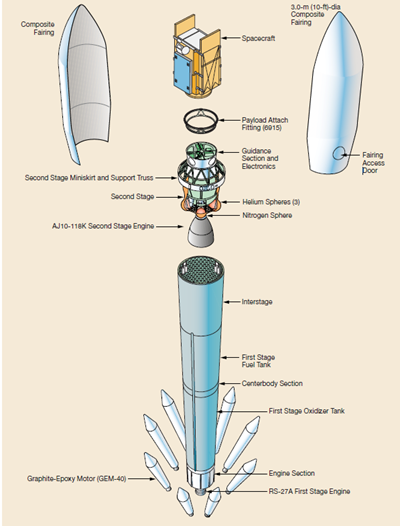
\includegraphics[width=.75\textwidth]{12-1.png}
\caption{Delta II 7920-10 Schematic. The 7320-10 is the same except it uses 3 strap-on boosters.~\cite{ref12_13}}
\label{L1}
\end{figure}

\begin{figure}[H]
\centering
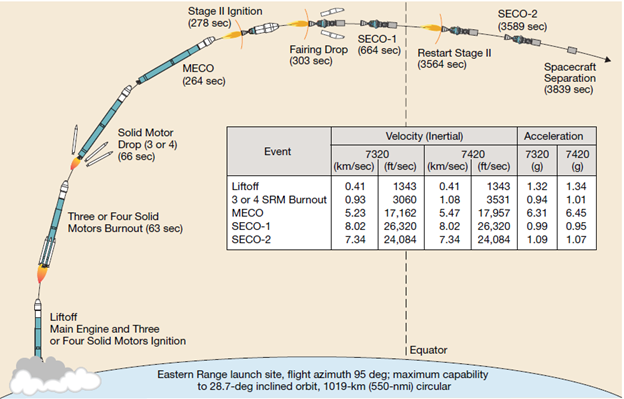
\includegraphics[width=.75\textwidth]{12-2.png}
\caption{Generic Delta II 7320 Mission Profile to Circular Orbit.}
\label{L2}
\end{figure}

The first stage of the rocket consists of the RS-27A engine, liquid oxygen and RP-1 fuel tanks, and the inter-stage. The RS-27A employs a 12:1 expansion ratio and the thrust chamber and nozzle are hydraulically gimbaled to provide pitch and yaw control. Roll control is provided by two Rocketdyne Vernier engines. The second stage contains the AJ10-1185 engine as well as the fuel (A-50) and oxidizer (NTO) tanks~\cite{ref12_14}. This stage also employs hydraulic gimbals for pitch and yaw control while a redundant attitude control system uses nitrogen gas for roll control during powered flight. In unpowered flight, the RACS provides control over the three rotations. The launch profile of a generic Delta II 7320 is shown in Figure~\ref{L2}. Here, the phase of each mission is indicated alongside times from launch. According to this figure, it will take 10 minutes to reach Second Engine Cut-off and approximately 1 hour for complete separation from the spacecraft.

\subsubsection{Payload Fairing and Interface}
\begin{figure}[H]
\centering
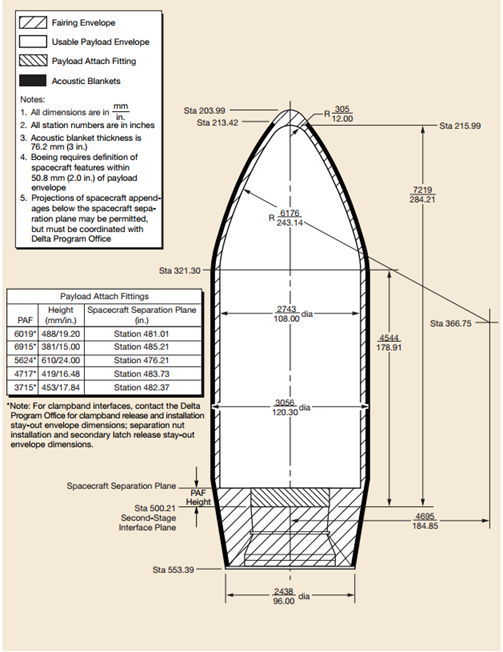
\includegraphics[width=.75\textwidth]{12-3.png}
\caption{Delta II 7320-10 Payload Fairing.}
\label{L3}
\end{figure}

In Figure~\ref{L3}, the payload fairing of the 7320-10 is shown with acoustic blanket padding created from melamine foam covered with reinforced carbon-loaded kapton face sheets. The 2.74 m inner diameter of the fairing allows for a snug fit of the 3.42 m tall HST reboost vehicle. The extra space will be sold to spaceflight to fill in with cubesats in order to offset monetary costs and to lessen g-loading on reboost vehicle. As a result, the analysis in the section 13 will assume full payload capacity when performing analysis.

%----------------------------------------------------------------------------------------
%	Spacecraft Structure
%----------------------------------------------------------------------------------------

\section{Spacecraft Structure} \label{section:structure}
\subsection{Structure Layout}
The structural layout for the HRV is shown below in Figures~\ref{fig:p1}-\ref{fig:p4}. The initial driving factor for the design is the requirement that the HRV interface with the SCM using the previously-developed LIDS system, with dimensions as described in Section~\ref{lids}.

The spacecraft exterior is covered in MMOD shielding on all six sides of the cube, and includes solar panels on four of the sides. Cold gas thrusters are strategically located at several corners for ADCS and rendezvous control. Sensors are located on the top (+Z) of the spacecraft for rendezvous maneuver determination with HST, and antennae are located on the bottom of the craft for communication.

In the spacecraft interior, the propulsion system includes two propellant tanks (one for each bipropellant), two helium pressurant tanks (one for each bipropellant), and two nitrogen cold gas tanks. The remainder of the ADCS system is located near the center of the craft. Also in the spacecraft are batteries, command and control computers, and plumbing and wiring.

The primary structure is a rectangular cube, and is made of extruded aluminum 6061-T6 beams with an external cubic dimension of 3 inch and a wall thickness of .125 inch. Aluminum 6061-T6 is a common material for spacecraft structures, due to its high strength-to-weight ratio, low cost, and machinability. for spacecraft structures, due to its high strength-to-weight ratio, low cost, and machinability. The design concept was chosen for its simplicity, manufacturability, stiffness, and reliability. Additional structural supports are used to hold hardware securely in the spacecraft. The overall dimensions of the cube of the spacecraft are 1.85 m x 1.85 m wide x 2.2 m tall. When including the docking mechanism and payload fairing attachment (not shown below), the overall height is 3.42 m.

\begin{figure}[H]
    \begin{center}
    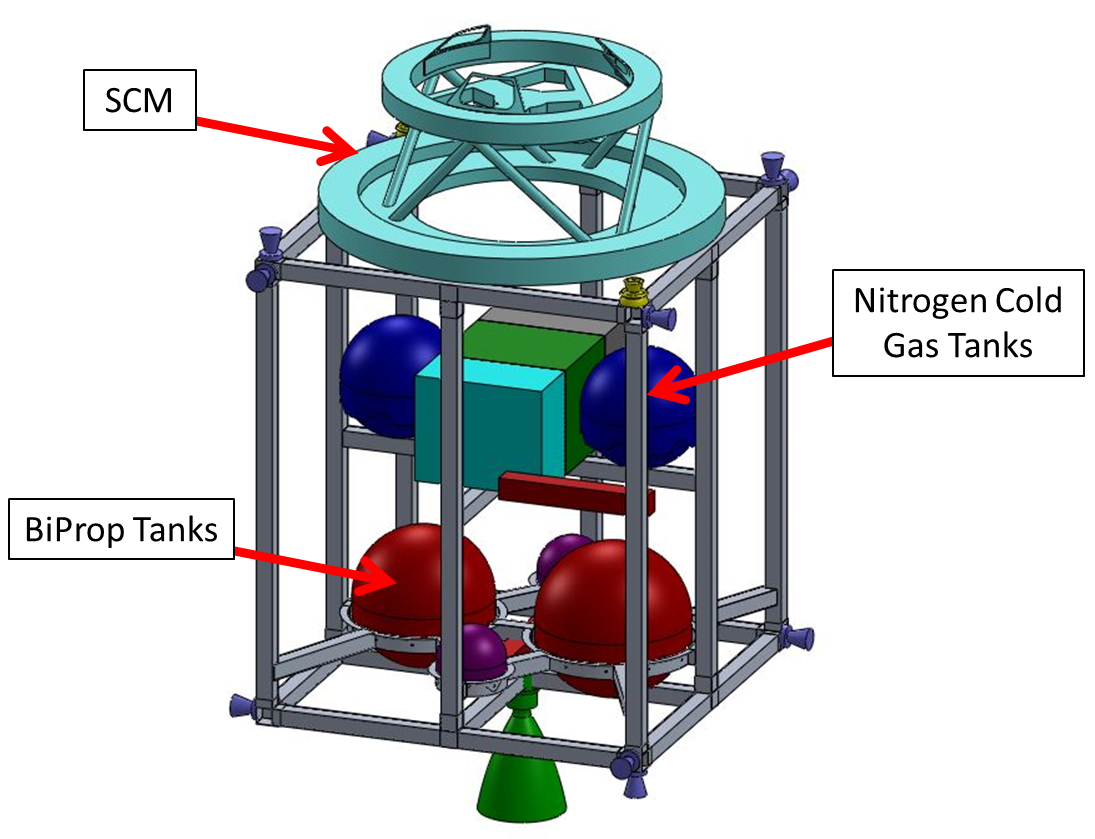
\includegraphics[width=0.5\textwidth]{Pics/1.png}
    \caption{HRV concept, view A, exterior shown.}
    \label{fig:p1}
    \end{center}
\end{figure}

\begin{figure}[H]
    \begin{center}
    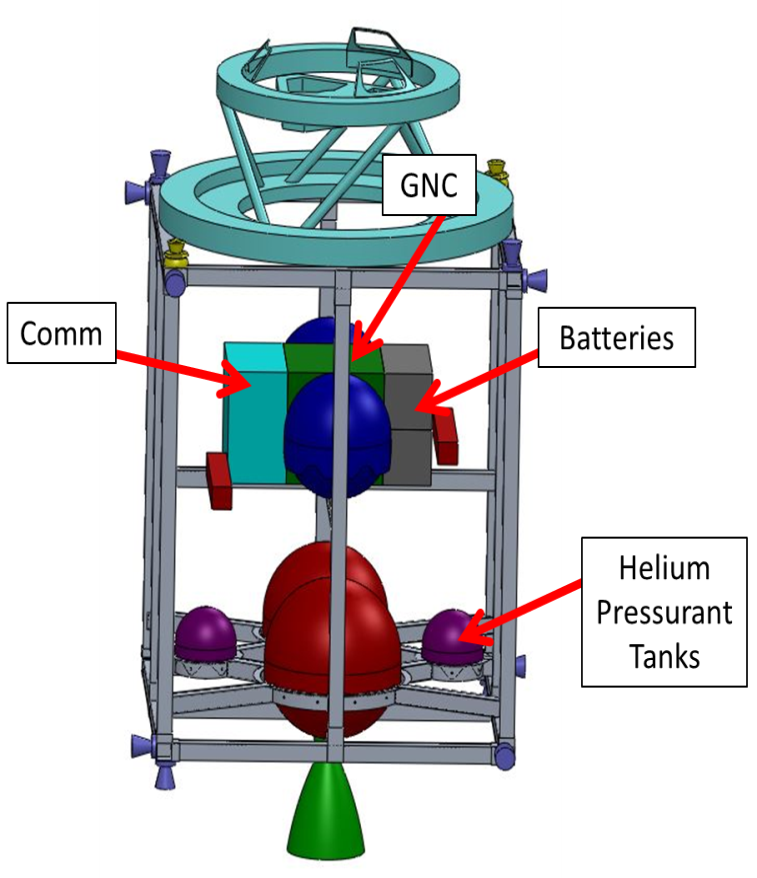
\includegraphics[width=0.5\textwidth]{Pics/2.png}
    \caption{HRV concept, view A, interior shown.}
    \label{fig:p2}
    \end{center}
\end{figure}

\begin{figure}[H]
    \begin{center}
    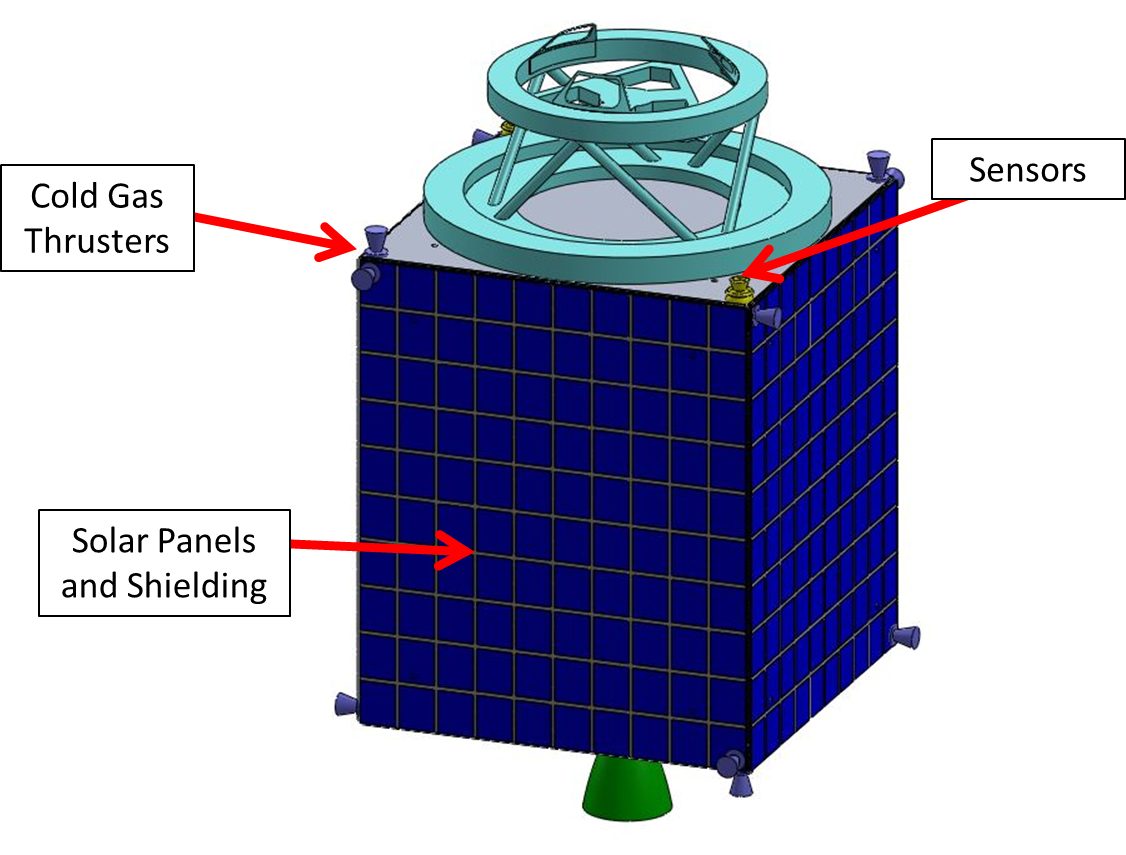
\includegraphics[width=0.5\textwidth]{Pics/3.png}
    \caption{HRV concept, view B, interior shown.}
    \label{fig:p3}
    \end{center}
\end{figure}

\begin{figure}[H]
    \begin{center}
    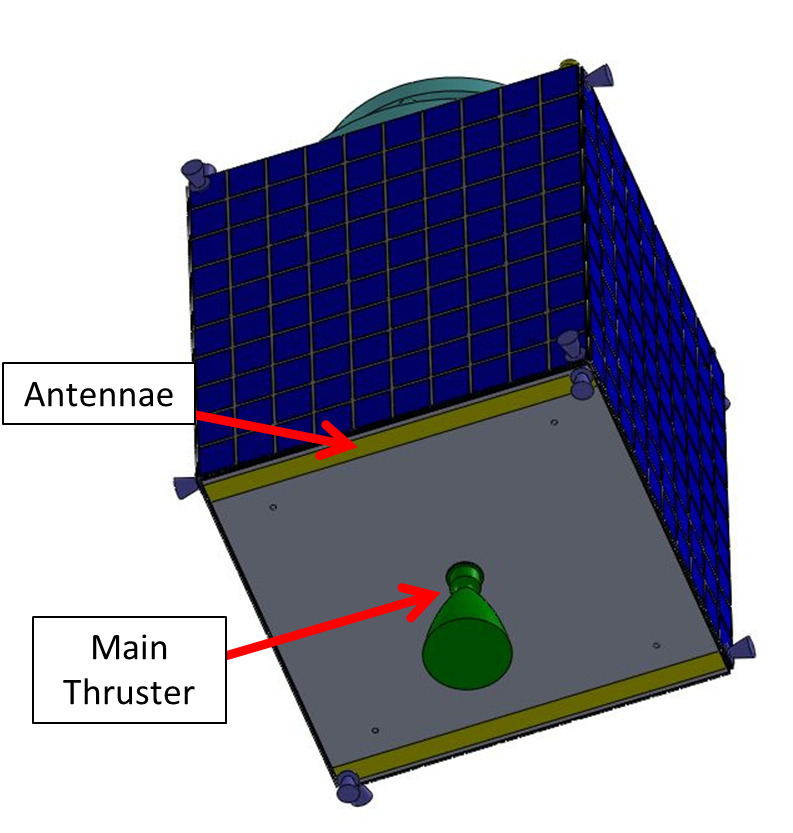
\includegraphics[width=0.5\textwidth]{Pics/4.png}
    \caption{HRV concept, view C, exterior shown.}
    \label{fig:p4}
    \end{center}
\end{figure}

The total estimated (dry and fueled) mass breakdowns of the spacecraft are shown in below

\begin{table}[H]
  \centering
  \begin{tabular}{l r}
    \toprule
    Item             & Mass (kg) \\
    \midrule
    MMH Tank         & 16.26     \\
    NTO (MON-3) Tank & 19.80     \\
    Cold Gas Tanks   & 40.33     \\
    Main Thruster    & 6.80      \\
    Pressurant Tanks & 6.87      \\
    Structure        & 73.40     \\
    Shielding        & 224.31    \\
    Solar Panels     & 25.00     \\
    SCM              & 75.00     \\
    ADCS             & 24.02     \\
    COMM             & 25.40     \\
    Batteries        & 7.00      \\
    Plumbing, Wiring & 14.00     \\
    Hardware         & 11.18     \\
    \midrule
    Total Dry Mass   & 569.36    \\
    \bottomrule
  \end{tabular}
  \caption{Estimated dry mass of HRV.}
  \label{table:dry_mass}
\end{table}

\begin{table}[H]
  \centering
  \begin{tabular}{l r}
    \toprule
    Item                & Mass (kg) \\
    \midrule
    Dry mass            & 569.36    \\
    MMH                 & 140.95    \\
    NTO (MON-3)         & 304.44    \\
    Pressurant (Helium) & 0.67      \\
    Cold Gas (Nitrogen) & 40.61     \\
    \midrule
    Total Launch Mass   & 1056.03   \\
    \bottomrule
  \end{tabular}
  \caption{Estimated fueled mass of HRV.}
  \label{table:fueled_mass}
\end{table}

With an origin in the center of the cube of the HRV, the estimated center of mass is located at -10.02 inches in the axial z direction, 2.547 inches in x, and .274 inches in y (shown below in Figure~\ref{fig:p5}).

\begin{figure}[H]
    \begin{center}
    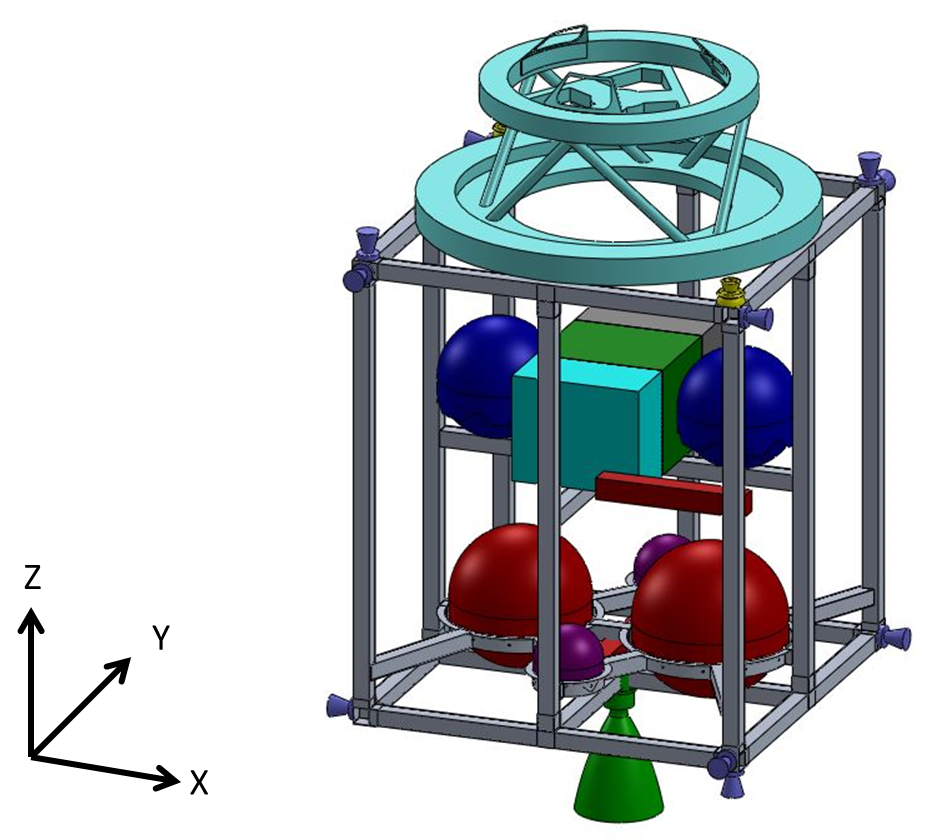
\includegraphics[width=0.5\textwidth]{Pics/5.png}
    \caption{Coordinate System.}
    \label{fig:p5}
    \end{center}
\end{figure}

\subsection{Analyses and Test Plans}
As stated in the requirements, the spacecraft structure must have a higher stiffness than the minimum determined by the launch provider, and must meet all stress criteria within the FOS for quasi-static and vibrational loading. As of this report, the structural design has been completed to a PDR level, with basic analyses performed to prove the concept of the design strength, but without detailed or optimized analyses that would come in the next stage of the project.

\subsubsection{Natural Frequency of Structure}
The minimum natural frequency of the HRV structure is defined by the launch vehicle provider. With the Delta II 7320-10 as the selected launch vehicle, the minimum allowable natural frequency is 35 Hz in the thrust direction and 20 Hz in the lateral directions~\cite{delta2}.

The structural design of the HRV uses aluminum extrusions with a wall thickness of .125 inches and an outer cube dimension of 3 inches, which results in a high stiffness. The natural frequencies were calculated with the payload mounted in the 5624 PAF. The first mode in the lateral direction is 46.3 Hz, while the first mode in the thrust direction is 57.9 Hz. The calculation process is shown below in Figure~\ref{fig:p6}. A calculator was developed for the natural frequencies and quasi-static load analyses, shown in Figure~\ref{fig:p7}. The structure is assumed to act as a cantilever beam in bending, with an equivalent point mass at the center of mass of the spacecraft.

\subsubsection{Quasi-Static Loads}

The maximum quasi-static loads are defined as 10.2 g in the axial direction (summation of 3.0 and 7.2) and 3.0 g in the lateral direction~\cite{delta2}. For the HRV spacecraft structure, quasi-static loads result in stress from axial force, bending stress, and shear stress. Buckling of individual structural members is also taken into consideration. With the current design, all cases meet FOS requirements. See Figure~\ref{fig:p7} and Figure~\ref{fig:p8} for calculations.

\begin{figure}[H]
    \begin{center}
    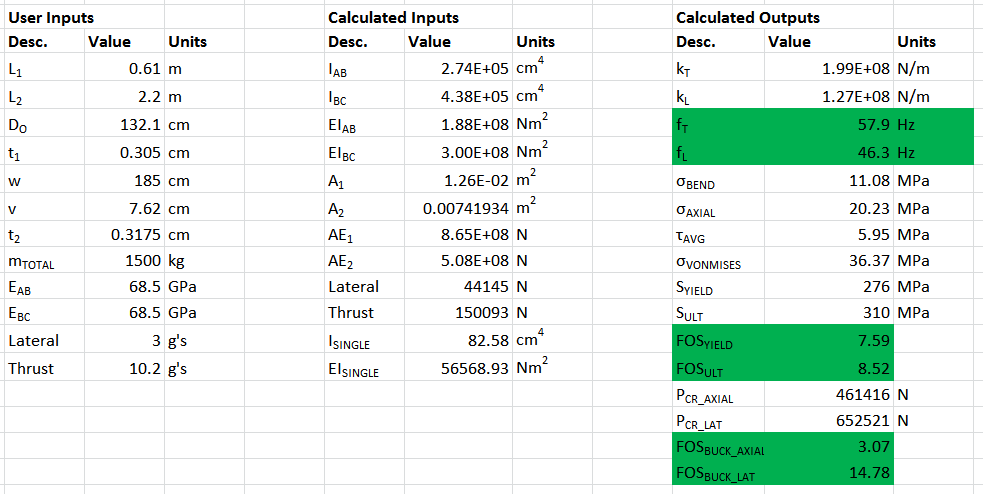
\includegraphics[width=1\textwidth]{Pics/7.png}
    \caption{Quasi-static stress analysis.}
    \label{fig:p7}
    \end{center}
\end{figure}

\begin{figure}[H]
    \begin{center}
    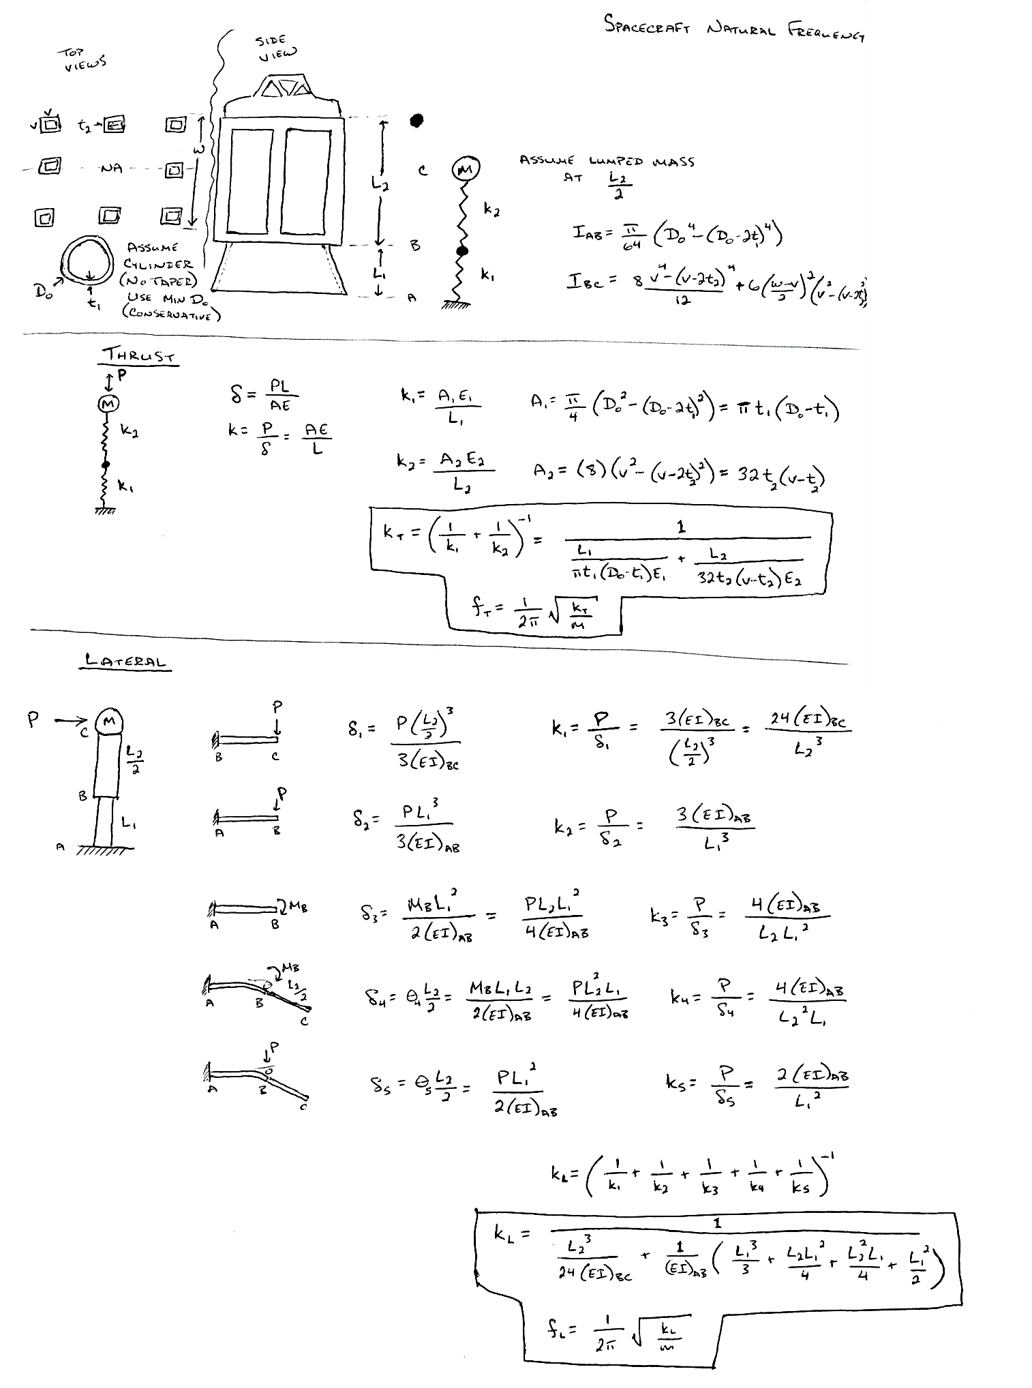
\includegraphics[width=1\textwidth]{Pics/freq.png}
    \caption{Natural frequency calculations for HRV.}
    \label{fig:p6}
    \end{center}
\end{figure}

\begin{figure}[H]
    \begin{center}
    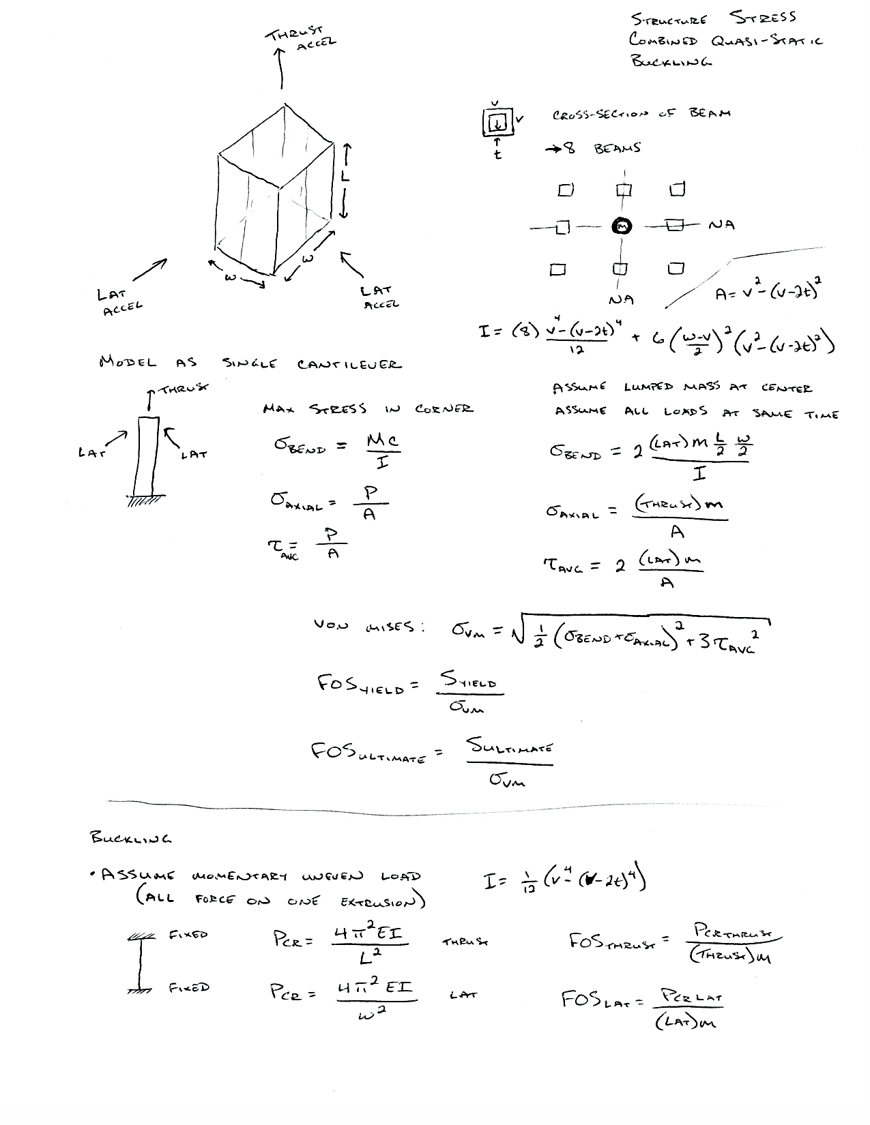
\includegraphics[width=1\textwidth]{Pics/stressbuckl.png}
    \caption{Quasi-static stress and buckling analyses.}
    \label{fig:p8}
    \end{center}
\end{figure}

\subsubsection{Vibration and Shock Loads}
Sinusoidal loads, random vibration loads, acoustic loads, and shock loads are beyond the scope of this PDR report. Sinusoidal loads for the Delta II at the HRV mass are lower than the quasi-static loads, and will therefore meet applicable margins of safety when performed after quasi-static load analyses. The shock response, random vibration power spectral density, and acoustic spectrum will depend on a more optimized design and analysis at a future point.

\subsubsection{Test Plans}
Qualification testing will be performed on a shaker table per the required loads, as defined in Section~\ref{section:reqs} of this report, and as defined by future specifications from the launch provider and the HRV team. Qualification testing will be performed at an amplification factor agreed upon with the launch provider.

\subsection{Solar Array Boom Deflection}

During this reboost mission, one of the mission objectives is to ensure that the maximum deflection of the solar panel arrays stays under 50 cm. This deflecting force occurs from the acceleration and mass of the panels while the reboost spacecraft is attached to HST, and at maximum thrust of 4000 N.

The current solar panels on the HST are the third iteration, and were installed during servicing mission 3B on STS-109 in 2002. The first two versions were very flexible, and could be rolled into the structural arm. A recorded video of an earlier reboost mission shows these panels undergoing an aggressive deformation. The current panel arrays are much more rigid, and are also about 30\% smaller. See Figures~\ref{fig:p9}-\ref{fig:p11}.

\begin{figure}[H]
    \begin{center}
    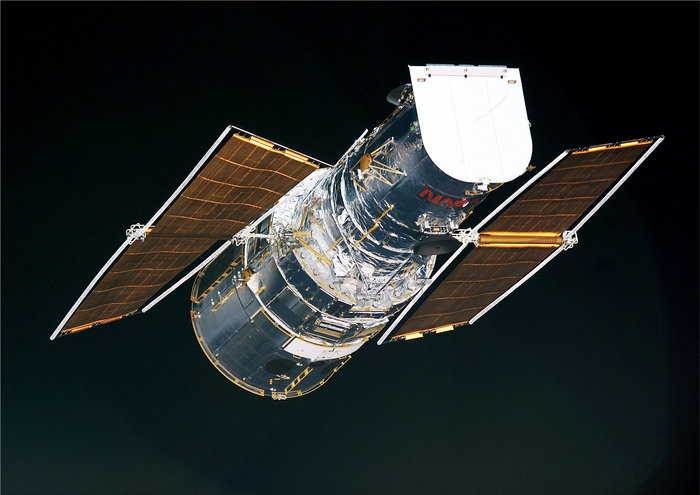
\includegraphics[width=0.6\textwidth]{Pics/9.png}
    \caption{Second iteration of solar panels, which were flexible.}
    \label{fig:p9}
    \end{center}
\end{figure}
%(http://www.esa.int/spaceinimages/Images/2010/12/Hubble_with_its_second_set_of_ESA-designed_solar_blankets)

\begin{figure}[H]
    \begin{center}
    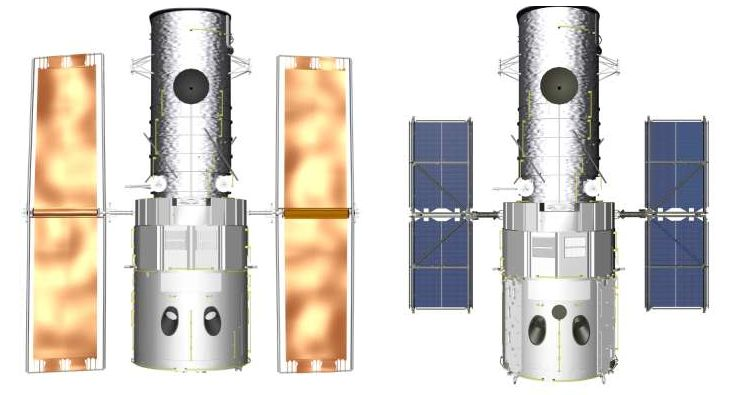
\includegraphics[width=0.5\textwidth]{Pics/10.png}
    \caption{Previous solar panel array (left) vs current solar panel array (right).}
    \label{fig:p10}
    \end{center}
\end{figure}
%http://asd.gsfc.nasa.gov/archive/sm3b/mission-critical/objectives-part2.html

\begin{figure}[H]
    \begin{center}
    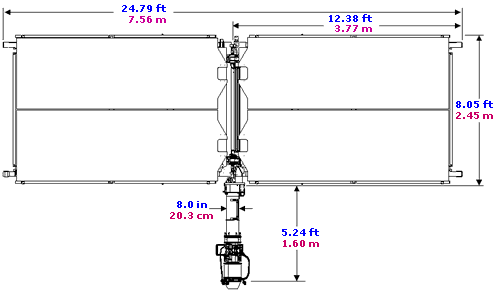
\includegraphics[width=0.5\textwidth]{Pics/11.png}
    \caption{Current solar panel array dimensions.}
    \label{fig:p11}
    \end{center}
\end{figure}
%http://asd.gsfc.nasa.gov/archive/hubble/art/shuttle_missions/sm3b/solpanel_measure.gif

Information taken from~\cite{csm}, \cite{mech3}, and Figure~\ref{fig:p11} was used to determine the design and material properties of the solar panel arrays. The deflection analysis was done with the following assumptions and descriptions

\begin{enumerate}
\item Both solar panel arrays are symmetric, so only one analysis is needed.
\item The solar panels will be oriented so that they are parallel to the axis of the Hubble (which is the orientation shown in Figure~\ref{fig:p10}). In this orientation, the long edge of the panels is in line with the thrusting force, so the induced bending moment is much lower than if they were rotated 90$^o$.
\item The arm which holds the solar panels is actually a complicated drive mechanism. It is modeled in this analysis as an aluminum shaft with a diameter of 4 cm, neglecting the surrounding mechanism.
\item The Hubble is a rigid structure in comparison, and calculated deflection begins at the base of the drive mechanism.
\item The array is modeled as a composite beam, as shown below in Figure~\ref{fig:p12} and Figure~\ref{fig:p13}
\begin{enumerate}
\item The drive mechanism shaft is beam AB, the middle double-extrusion section is beam BC, and the extrusion from the midspan to the tip of the array is beam CD.
\item Beam AB is a round aluminum shaft
\begin{enumerate}
\item   E = 68.5 GPa
\item $I = \frac{\pi d^4}{64}$
\end{enumerate}
\item Beam BC is a pair of extrusions made of Al-Li Alloy X2096-T8A3
\begin{enumerate}
\item   E = 75.15 GPa
\item $I = 2 \left(\frac{bh^3-(b-2t)(h-2t)^3}{12} + y^2(bh - (b-2t)(h-2t)) \right)$
\end{enumerate}
\item Beam CD is modeled as a rigid structure, as it is in line with the thrust force and should not experience bending. Axial deflection is not considered to be significant.
\item The maximum deflection is at point D (which is equivalent to the deflection at the bottom right corner in Figure~\ref{fig:p12}.)
\item It is assumed the solar panels themselves do not contribute to the stiffness of the structure, and that the area moment of inertia of beam BC is not increased due to a shear tie with the beam that runs parallel to CD from point B. Both of these are overly-conservative assumptions.
\item The transverse distributed loads found as follows
\begin{enumerate}
\item $Acceleration = \frac{Thrust}{Mass_{Hubble}}$
\item $\frac{Force}{Length} = \frac{Mass \times Acceleration}{Length_{Beam}}$
\item For the acceleration, the mass used is only for the Hubble. While the reboost spacecraft also has mass, its launch mass is \textless 10\% of the Hubble's, and it will have used most of its fuel by the end of the boost, so its mass will be \textless 5\% of the Hubble's. Neglecting the mass of the reboost spacecraft gives a slightly higher (and conservative) acceleration value.
\item For beam AB, the mass is of the drive mechanism.
\item For beam BC, the mass is of the structural beams and solar panels.
\end{enumerate}
\end{enumerate}
\item Using superposition, the deflection of point D is due to the summation of the components listed in Figure~\ref{fig:p13}. A spreadsheet calculator was made and used to perform this calculation at different thrust levels, and is shown in Figure~\ref{fig:p14}.
\end{enumerate}

\subsection{Results/Discussion}
With a maximum thrust of the chosen rocket engine of 4000 N, the maximum mechanical deflection on the boom structure is calculated at 11.10 cm. This is much lower than the allowable deflection of 50 cm, giving a factor of safety of 4.50.

It is preferable to have a high factor of safety in this situation, as there may be additional components to movement of the solar array other than structural deflection
\begin{enumerate}
\item The gearing in the drive mechanism at AB may have some play, allowing for a small amount of slippage under an abnormal load.
\item There is a titanium flexure at point B, which is designed to provide stress relief during rapid heating (thermal induced stresses). The stiffness of this flexure in the described bending situation is not clear.
\end{enumerate}

With the assumption that the main threat to the health of the solar panels is from mechanical deformation and not slippage or a localized flexible point, the maximum allowable thrust is calculated to be 18012 N, at which point the deflection would be 50 cm.

\begin{table}[H]
\centering
\begin{tabular}{l l}
\toprule
Design thrust & 4000 N \\
Design deflection & 11.10 cm \\
Factor of safety & 4.50 \\
Maximum thrust ($\delta=50$cm) & 18012 N \\
\bottomrule
\end{tabular}
\caption{Solar Array Boom Deflection Summary.}
\label{table:solar_deflection}
\end{table}

\begin{figure}[H]
    \begin{center}
    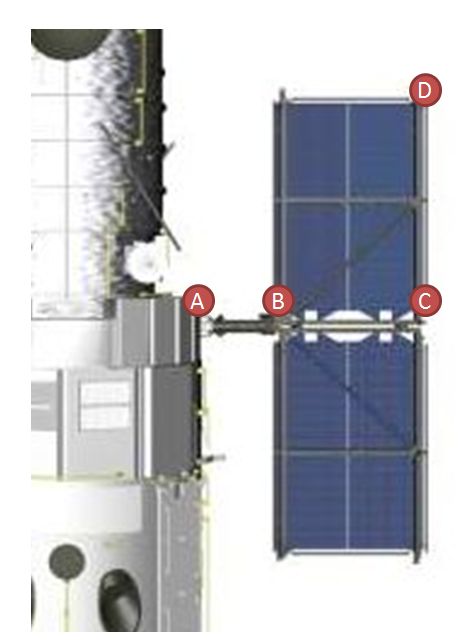
\includegraphics[width=0.4\textwidth]{Pics/12.png}
    \caption{Picture of Hubble solar array with labels corresponding to diagram.}
    \label{fig:p12}
    \end{center}
\end{figure}

\begin{figure}[H]
    \begin{center}
    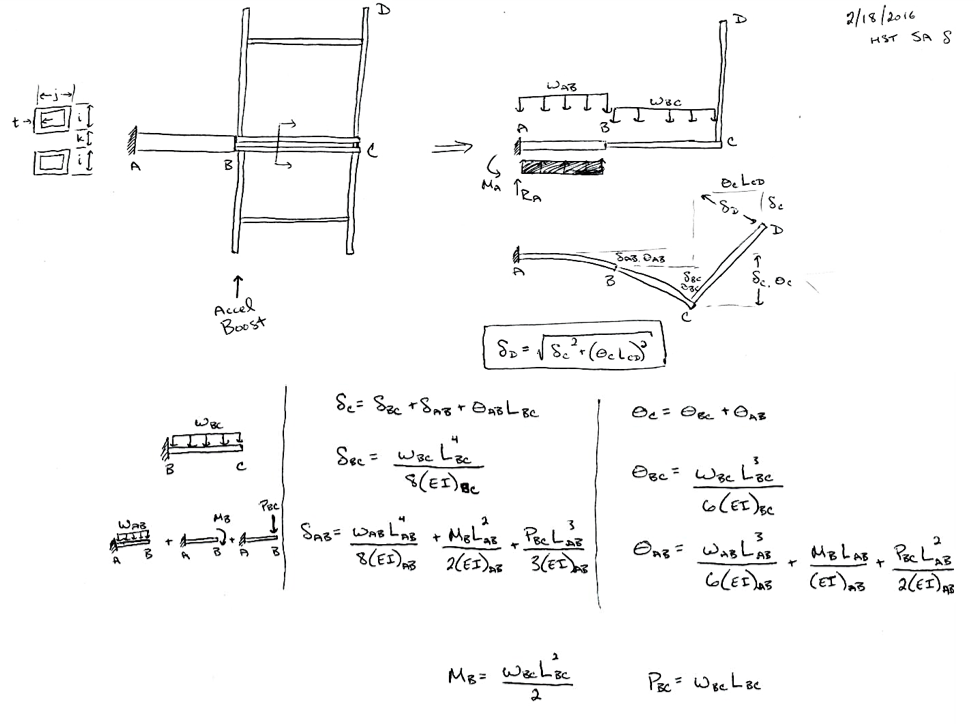
\includegraphics[width=.8\textwidth]{Pics/boomdefl.png}
    \caption{Diagrams and equations used for solar array deflection calculation (order of calculations is from bottom to top).}
    \label{fig:p13}
    \end{center}
\end{figure}

\begin{figure}[H]
    \begin{center}
    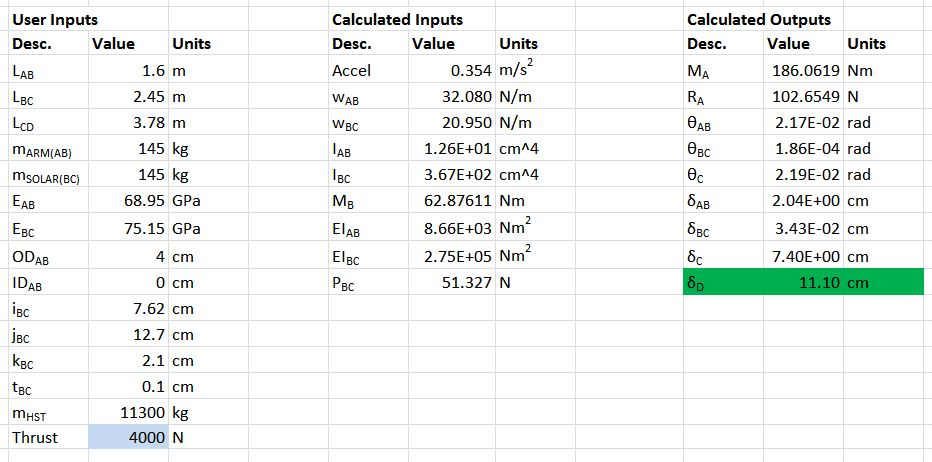
\includegraphics[width=.8\textwidth]{Pics/14.png}
    \caption{Spreadsheet used to calculate solar array deflection.}
    \label{fig:p14}
    \end{center}
\end{figure}

\subsection{Shock and Payload Attachment Fitting Selection}

According to SMAD, shock is a ``sharp, intense transient acceleration with broad frequency content and a very short duration''~\cite{ref12_8}. Compared to spacecraft separation the Delta II payload planner states that all other flight shock events, such as stage separation and engine ignition, are not significant. A noted feature of shock is that it does not transmit through structural joints and attenuates rapidly over distance. The amount of shock produced can be mitigated against depending on the choice of payload attachment fitting (PAF).

To reduce developmental time and cost, the manufacture provided PAFs in Table~\ref{13.1} will be considered. Their shock response spectrums (SRS) are shown in Figure~\ref{fig:13.1}-\ref{fig:13.3}, where it is seen that the 5624 PAF has the most suitable response for the HRV.

\begin{table}[H]
\centering
\begin{tabular}{l l}
\toprule
Payload Attachment Fitting & Separation System (diameter [mm], Type) \\
\midrule
3715 & 939.8, V-block Clamp \\
6306 & 1600, V-block Clamp \\
6019 & 1524, Three Explosive Separation Nuts \\
6915 & 1752.6, Four Explosive Separation Nuts \\
5624 & 1422.4, V-block Clamp \\
\bottomrule
\end{tabular}
\caption{List of Two-Stage Delta II PAFs.}
\label{13.1}
\end{table}

\begin{figure}[H]
    \begin{center}
    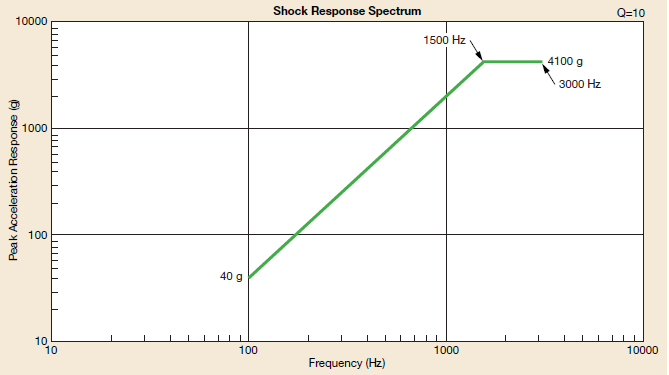
\includegraphics[width=.75\textwidth]{SS13_Shock_PAF/13-1.png}
    \caption{6306 PAF SRS.}
    \label{fig:13.1}
    \end{center}
\end{figure}

\begin{figure}[H]
    \begin{center}
    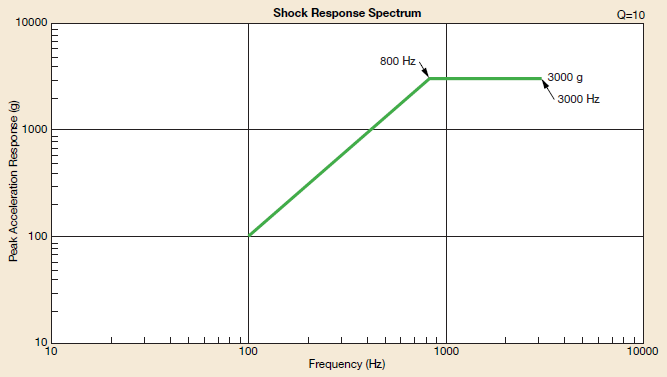
\includegraphics[width=.55\textwidth]{SS13_Shock_PAF/13-2.png}
    \caption{6306 PAF SRS.}
    \label{fig:13.2}
    \end{center}
\end{figure}

\begin{figure}[H]
    \begin{center}
    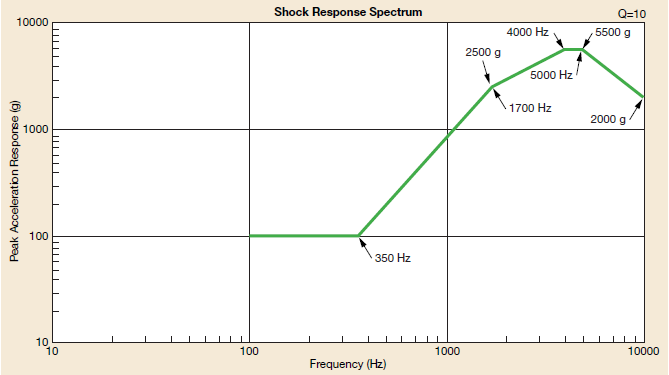
\includegraphics[width=.55\textwidth]{SS13_Shock_PAF/13-3.png}
    \caption{6019 and 6915 PAFs SRS.}
    \label{fig:13.3}
    \end{center}
\end{figure}

\begin{figure}[H]
    \begin{center}
    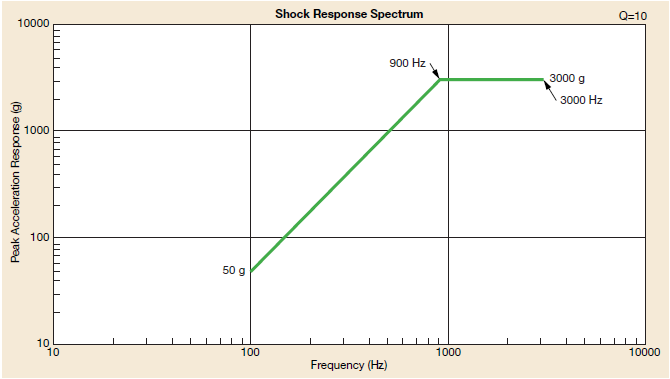
\includegraphics[width=.55\textwidth]{SS13_Shock_PAF/13-4.png}
    \caption{5624 PAF SRS.}
    \label{fig:13.4}
    \end{center}
\end{figure}

As indicated by its name the 5624 PAF, shown in Figure~\ref{fig:13.5}, is 56 inches (1422.4 mm) in diameter and 24 inches (609.6 mm) high. The interface employs the release of a V-band clamp and the action of four separation spring actuators to separate the HRV from the launch vehicle. The capability of the PAF is shown in Figure~\ref{fig:13.6}.

\begin{figure}[H]
    \begin{center}
    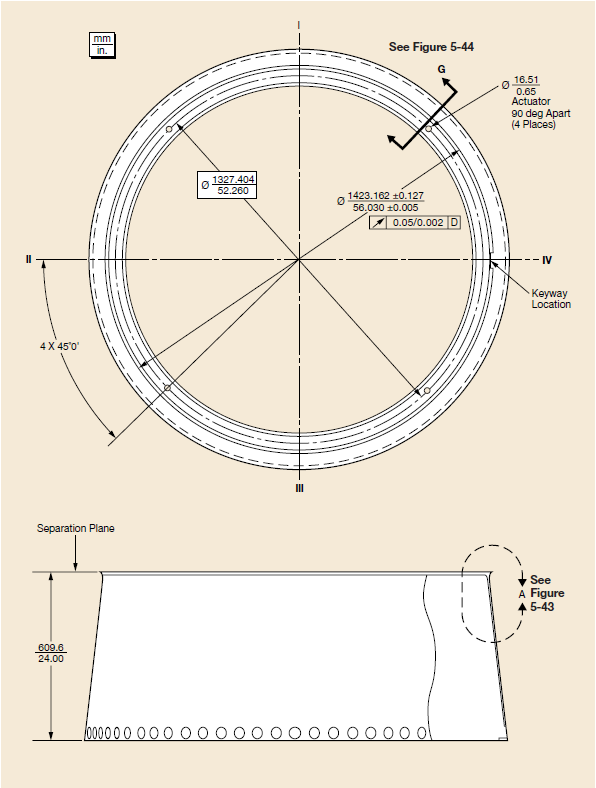
\includegraphics[width=.75\textwidth]{SS13_Shock_PAF/13-5.png}
    \caption{Delta II PAF selected for the HRV.}
    \label{fig:13.5}
    \end{center}
\end{figure}

\begin{figure}[H]
    \begin{center}
    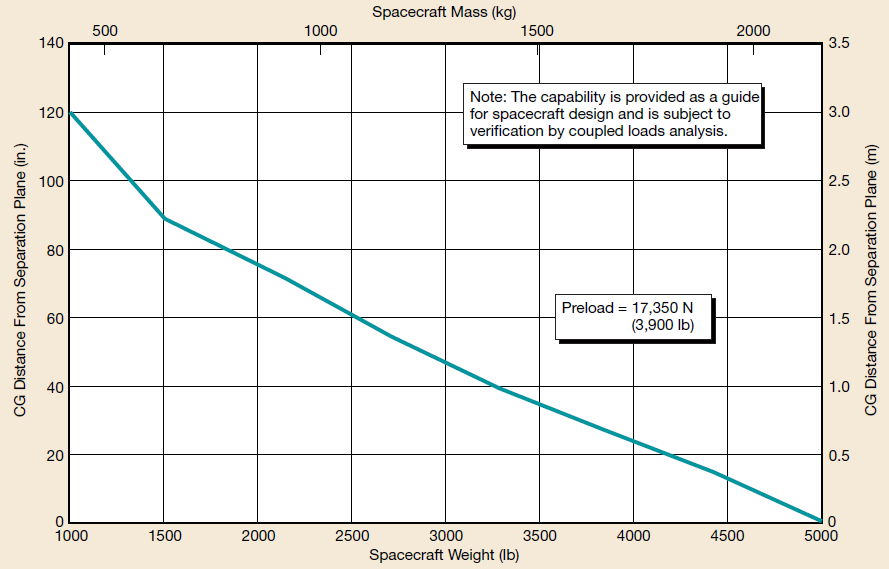
\includegraphics[width=.75\textwidth]{SS13_Shock_PAF/13-6.png}
    \caption{5624 PAF Capability.}
    \label{fig:13.6}
    \end{center}
\end{figure}

\subsubsection{Test Plan}

Shock testing is discussed in the Delta II payload planner's guide, where the PAF is activated twice while connected to the spacecraft~\cite{delta2}. This direct method is used similarly for both spacecraft qualification and acceptance testing and will be performed by the Delta Launcher company for us. To further verify structural soundness of the spacecraft-PAF system, a coupled-loads analysis will be performed.

%----------------------------------------------------------------------------------------
%	MMOD
%----------------------------------------------------------------------------------------

\section{MMOD Shielding}
In order to accurately design MMOD shielding first it must be known what to design for. For that reason a statistical orbital debris model will be used to find a critical particle diameter, which the shielding will be designed to resist without failing. To design the shielding the NASA MMOD handbook, and the NASA Shield Analysis Program are used. A trade study is conducted to select the shielding for the spacecraft based on volume, mass and materials used.

\subsection{Statistical Debris Model}
NASA's ORDEM v3 orbital debris modeling software was used to find the debris flux for all the relevant mission orbits~\cite{debris_model}. The three orbits analyzed for orbital debris include: the parking orbit, the transfer orbit, and Hubble's orbit. It was found that Hubble's orbit has the largest orbital debris flux, which can be seen in Figure~\ref{fig:hubbleOrbit}. This is most likely because the other two orbits have a perigee at 200 km, where there is enough drag to slowly deorbit most debris. At 550 km however debris will not deorbit for a long time, and could damage the spacecraft.

\begin{figure}[H]
	\begin{center}
	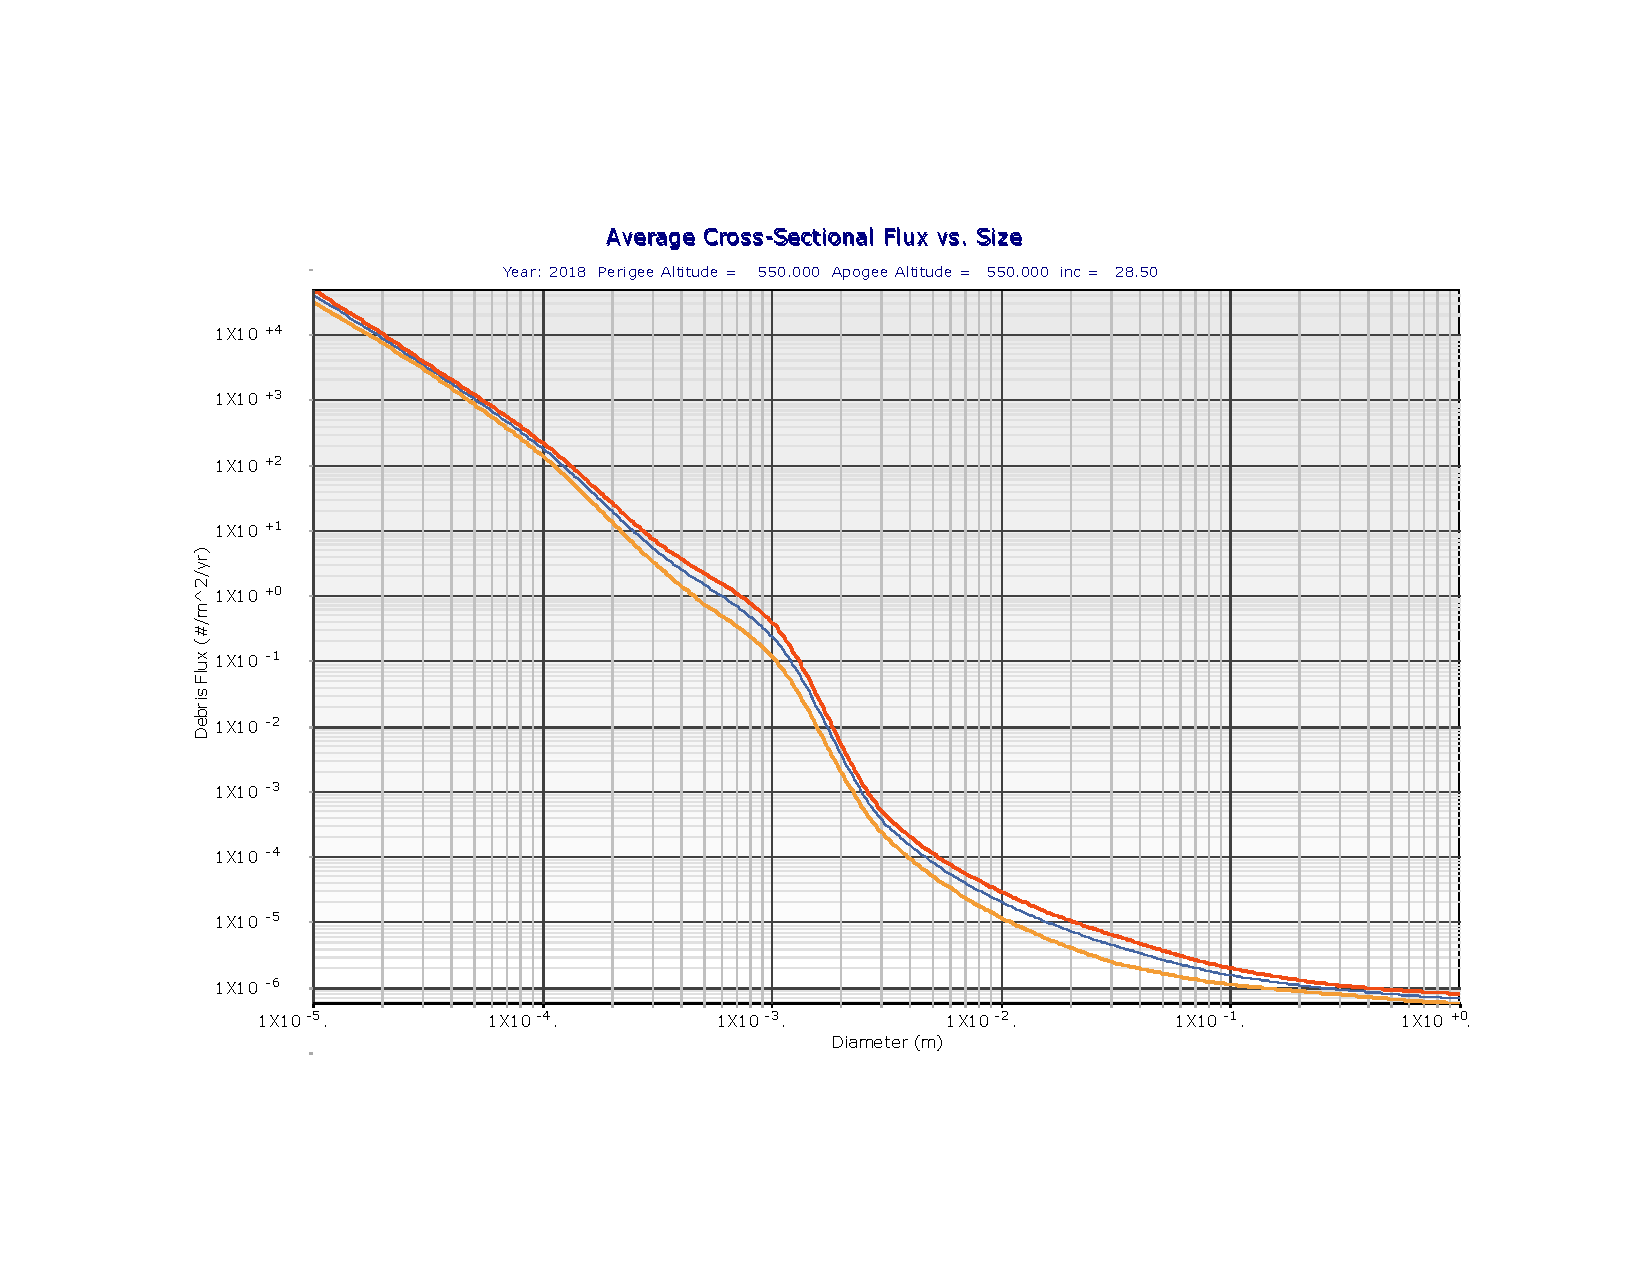
\includegraphics[width=5.5in]{hstOrbit.pdf}
	\caption{Orbital debris flux for Hubble's orbit in 2018.}
	\label{fig:hubbleOrbit}
	\end{center}
\end{figure}

To find out what size of particle to design the Debris flux must be found for the spacecraft given a probability of no impact. From the NASA Handbook for Designing MMOD Protection~\cite{handbook_mmod} probability of no penetration is defined by following equations

\begin{equation*}
PNP = e^{-N}
\end{equation*}
where
\begin{equation*}
N = \sum\limits_{i=1}^n (FAt)_i
\end{equation*}

In the equations, $N$ is the number of impacts, $F$ (number/m$^2$-year) is the cumulative flux, $A$ (m$^2$) is the exposed area of the spacecraft, and $t$ (years) is the exposure time. For the reboost vehicle a two week mission was used, with a probability of no penetration of 99.99\% (which is less than a occurrence level E in the FMEA), and an exposed area of 4.07 meters. These figures are used to calculate a debris flux density of $7.7 x 10^{-4}$. Using this value and Figure~\ref{fig:hubbleOrbit} the critical particle diameter was found to be approximately 0.27 cm.

\subsection{Shielding Design}
The MMOD shielding was designed to withstand a steel particle traveling at 15 km/s with a diameter of 0.27 cm hitting perpendicular to the shielding. The particle diameter comes from the statistical model, and the velocity is calculated assuming the orbital debris is flying in the same circular orbit as the reboost vehicle, but in the exact opposite direction.

Using the NASA Shield Analysis Program many shields were calculated using the above criteria~\cite{ryan2010micrometeoroid}. To calculate the weight the areal shielding density can be multiplied times the surface area of the spacecraft, where the surface area is 23.13 m$^2$. In Tables~\ref{table:solidMMOD} and \ref{table:MMOD} Al6061-T6 was used for all bumpers, and Al7075-T6 was used for all walls. This was because the hardness of Al7075 is significantly higher, which is needed for the wall layer, but not for the bumpers. Nextel was used when composite shielding decision was to be made.
% TABLE FOR .999 PNP
% \begin{table}[H]
% \begin{centering}
% \begin{tabular}{lrr}
% 	Type of Solid Shield & areal density & thickness \\ \hline
% 	Metallic             & $5.77 g/cm^2$ & $2.06 cm$ \\
% 	Composite            & $4.60 g/cm^2$ & $3.23 cm$ \\
% \end{tabular}
% \caption{Areal density for solid MMOD shielding.}
% \label{table:solidMMOD}
% \end{centering}
% \end{table}

% \begin{table}[H]
% \begin{centering}
% \begin{tabular}{lccc}
%                          & \multicolumn{3}{c}{Shield Overall Thickness}  \\
% 	Type of Shield       & 3 in          & 5 in          & 8 in \\ \hline
% 	Whipple              & 0.89 $g/cm^2$ & 0.77 $g/cm^2$ & 0.67 $g/cm^2$ \\
% 	Honeycomb Sandwich   & 2.89 $g/cm^2$ & 2.24 $g/cm^2$ & 1.77 $g/cm^2$ \\
% 	Triple Wall Whipple  & 1.21 $g/cm^2$ & 0.88 $g/cm^2$ & 0.65 $g/cm^2$ \\
% 	Nextel Multi-Shock   & 0.69 $g/cm^2$ & 0.31 $g/cm^2$ & 0.31 $g/cm^2$ \\
% 	Aluminum Multi-Shock & 0.88 $g/cm^2$ & 0.68 $g/cm^2$ & 0.54 $g/cm^2$ \\
% 	Stuffed Whipple      & 0.67 $g/cm^2$ & 0.63 $g/cm^2$ & 0.62 $g/cm^2$ \\
% \end{tabular}
% \caption{Areal density for MMOD shielding.}
% \label{table:MMOD}
% \end{centering}
% \end{table}

% TABLE FOR .9999 PNP
\begin{table}[H]
\begin{centering}
\begin{tabular}{lrr}
\toprule
	Type of Solid Shield & Material Density & Thickness \\
\midrule
	Metallic             & 7.92 g/cm$^2$ & 2.83 cm \\
	Composite            & 6.20 g/cm$^2$ & 4.36 cm \\
\bottomrule
\end{tabular}
\caption{Areal density for solid MMOD shielding.}
\label{table:solidMMOD}
\end{centering}
\end{table}

\begin{table}[H]
\begin{centering}
\begin{tabular}{lccc}
\toprule
                         & \multicolumn{3}{c}{Shield Overall Thickness}  \\
\midrule
	Type of Shield       & 3 in          & 5 in          & 8 in \\ \hline
	Whipple              & 1.45 g/cm$^2$ & 1.13 g/cm$^2$ & 0.99 g/cm$^2$ \\
	Honeycomb Sandwich   & 4.54 g/cm$^2$ & 3.51 g/cm$^2$ & 2.78 g/cm$^2$ \\
	Triple Wall Whipple  & 2.01 g/cm$^2$ & 1.48 g/cm$^2$ & 1.12 g/cm$^2$ \\
	Nextel Multi-Shock   & 1.35 g/cm$^2$ & 0.75 g/cm$^2$ & 0.54 g/cm$^2$ \\
	Aluminum Multi-Shock & 1.38 g/cm$^2$ & 1.07 g/cm$^2$ & 0.85 g/cm$^2$ \\
	Stuffed Whipple      & 0.97 g/cm$^2$ & 0.88 g/cm$^2$ & 0.85 g/cm$^2$ \\
\bottomrule
\end{tabular}
\caption{Areal density for MMOD shielding.}
\label{table:MMOD}
\end{centering}
\end{table}

Table~\ref{table:MMOD} shows a trade off that happens between the overall mass of the shielding and its thickness. This is because when debris hits the shielding at high speeds it evaporates and creates a plume of material that sprays to the next layer. The more that plume is able to spread out, which is directly correlated to shield thickness, the thinner the final wall can be. An example of the plume can be seen in Figure~\ref{fig:plume}.

\begin{figure}[H]
	\begin{center}
	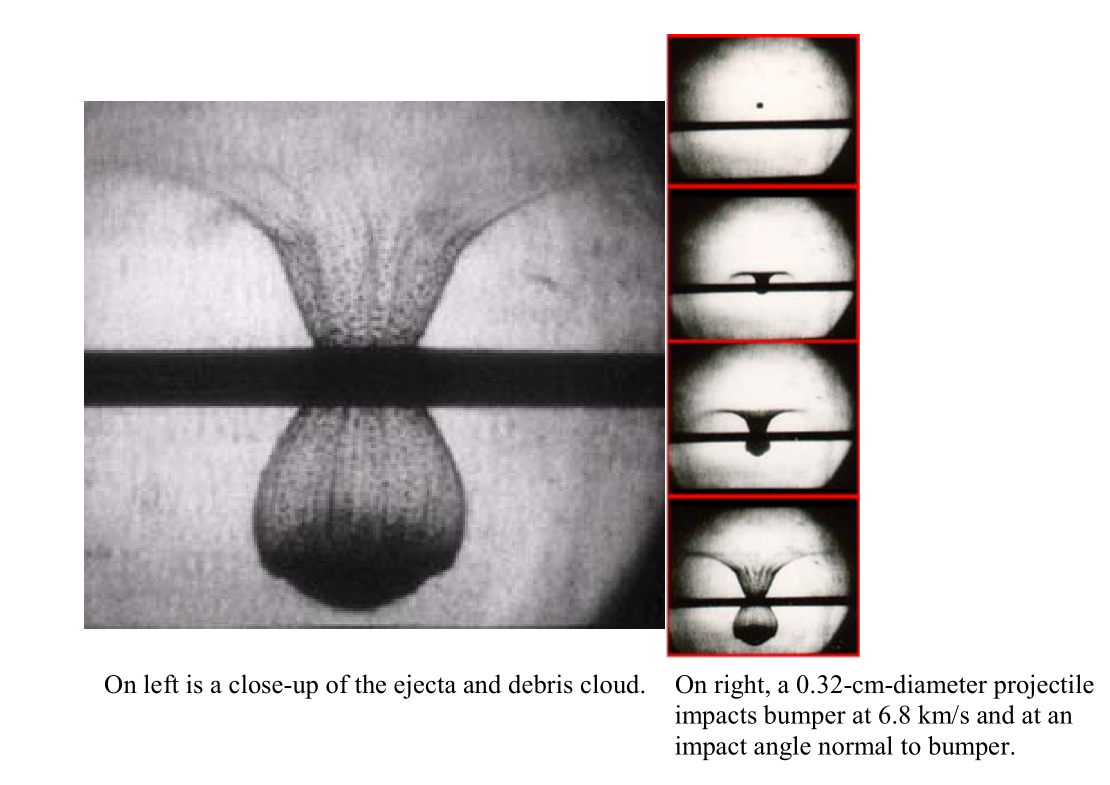
\includegraphics[width=5in]{plume.png}
	\caption{Debris cloud observed in high-speed camera film.}
	\label{fig:plume}
	\end{center}
\end{figure}

The first design decision made was the shielding thickness. To integrate with the reboost spacecraft, the shielding should be able to fit in between the structural members, which are 3 inches thick. The shielding, however, can extend past the structural elements by welding it onto a standoff attached to the structural member. If the shielding does extend past the edge of the spacecraft it shouldn't do so by much, since at that point it's expanding the profile of the spacecraft. Based on Table~\ref{table:MMOD} only a few shielding decisions appear a good option to keep weight low. Both the 5 inch stuffed whipple and nextel multi-shock give a good strength to weight ratio as well as the 3 inch thick stuffed whipple. All of these shields have been plotted side by side for a more in depth comparison with regard to their ballistic limit curves.

\begin{figure}[H]
	\begin{center}
	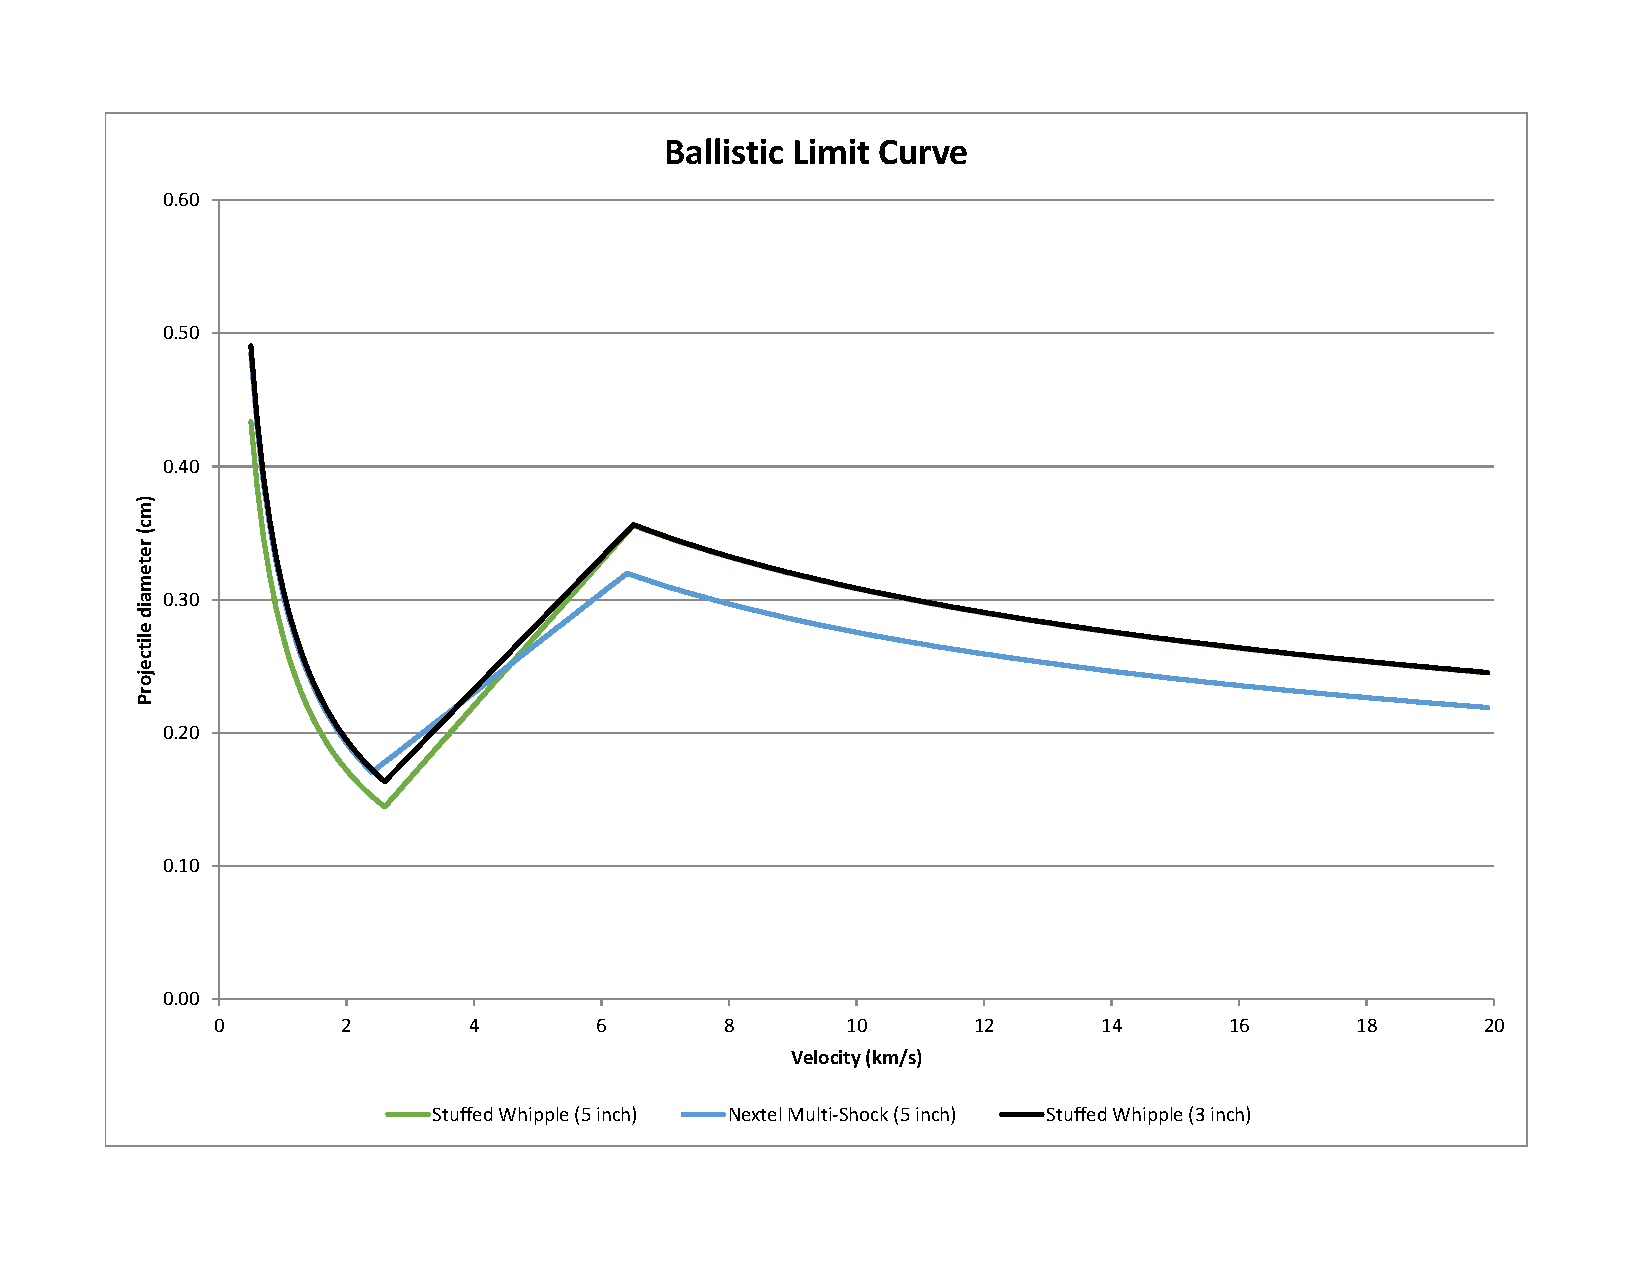
\includegraphics[width=5in]{BallisticLimit.pdf}
	\caption{Ballistic limit curve for MMOD shielding.}
	\label{fig:ballisticLimit}
	\end{center}
\end{figure}

Figure~\ref{fig:ballisticLimit} shows that the stuffed whipple provides more protection at higher collision velocities, and the 3 inch version is able to stay within the structure thickness. This makes the 3 inch thick stuffed whipple the ideal candidate to move forward with.

Each layer of the whipple shield adds a new plume of material to be distributed to the next. As seen in Figure~\ref{fig:stuffedWhipple} the stuffed whipple shield has a traditional bumper and rear wall, but with a kevlar and nextel layer in the middle. The composite nextel material excels at stopping debris moving fast enough to vaporize the bumper and immediately create a plume. When the debris is moving slowly the stuffing doesn't provide much extra protection over a standard whipple shield. This can be seen in Figure~\ref{fig:ballisticLimit} where the high range of velocities have a fairly large critical diameter and the lower collision velocities have a smaller collision diameter.

\begin{figure}[H]
	\begin{center}
	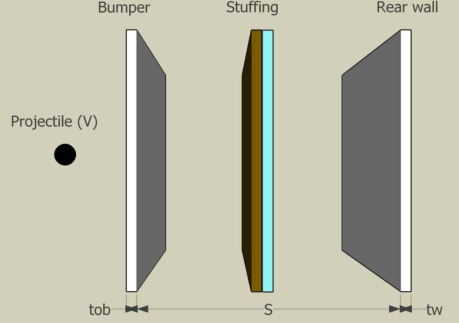
\includegraphics[width=3in]{stuffedWhipple.png}
	\caption{Stuffed Whipple shield configuration.}
	\label{fig:stuffedWhipple}
	\end{center}
\end{figure}

The shielding shall be created to the specifications in Table~\ref{table:stuffedWhippleDesign}.

\begin{table}[H]
\begin{centering}
\begin{tabular}{lrr}
\toprule
Description                        & Units    & Value  \\ \hline
\midrule
Bumper plate thickness             & cm     & 0.1208 \\
Nextel areal density               & g/cm$^2$ & 0.3749 \\
Kevlar areal density               & g/cm$^2$ & 0.1250 \\
Total stuffing area density        & g/cm$^2$ & 0.4999 \\
Rear wall thickness                & cm     & 0.0499 \\
Shield areal weight                & g/cm$^2$ & 0.9655 \\
Spacing (front bumper to stuffing) & cm     & 3.81   \\
Spacing (stuffing to rear wall)    & cm     & 3.81   \\
Total Shielding Mass               & kg     & 224.31 \\
\bottomrule
\end{tabular}
\caption{Stuffed design parameters.}
\label{table:stuffedWhippleDesign}
\end{centering}
\end{table}

\subsection{Spacecraft Structure}
As the structural members are also exposed to MMOD, an additional analysis was conducted to ensure that the HRV structure is able to withstand orbital debris. The structure has a much smaller upwind surface area meaning that the debris flux is smaller than that of the entire spacecraft. Using figure \ref{fig:hubbleOrbit} it was found that the structure must withstand a maximum debris diameter of 0.2 cm.

To provide an extra layer of protection for the spacecraft structure the MMOD bumper and wall will be solid sheets that go over and under the structural members. This will give the structure extra thickness to prevent debris from penetrating the spacecraft. For calculation purposes this arrangement can be approximated as a whipple shield.

With the summed wall thicknesses NASA Shield Analysis Program was used to generate a ballistic limit curve for the spacecraft structure using the same projectile speed and material as the original analysis. Figure \ref{fig:MMODstructure} shows that the structure is capable of withstanding the new critical particle diameter and keeping system components safe.

\begin{figure}[H]
	\begin{center}
	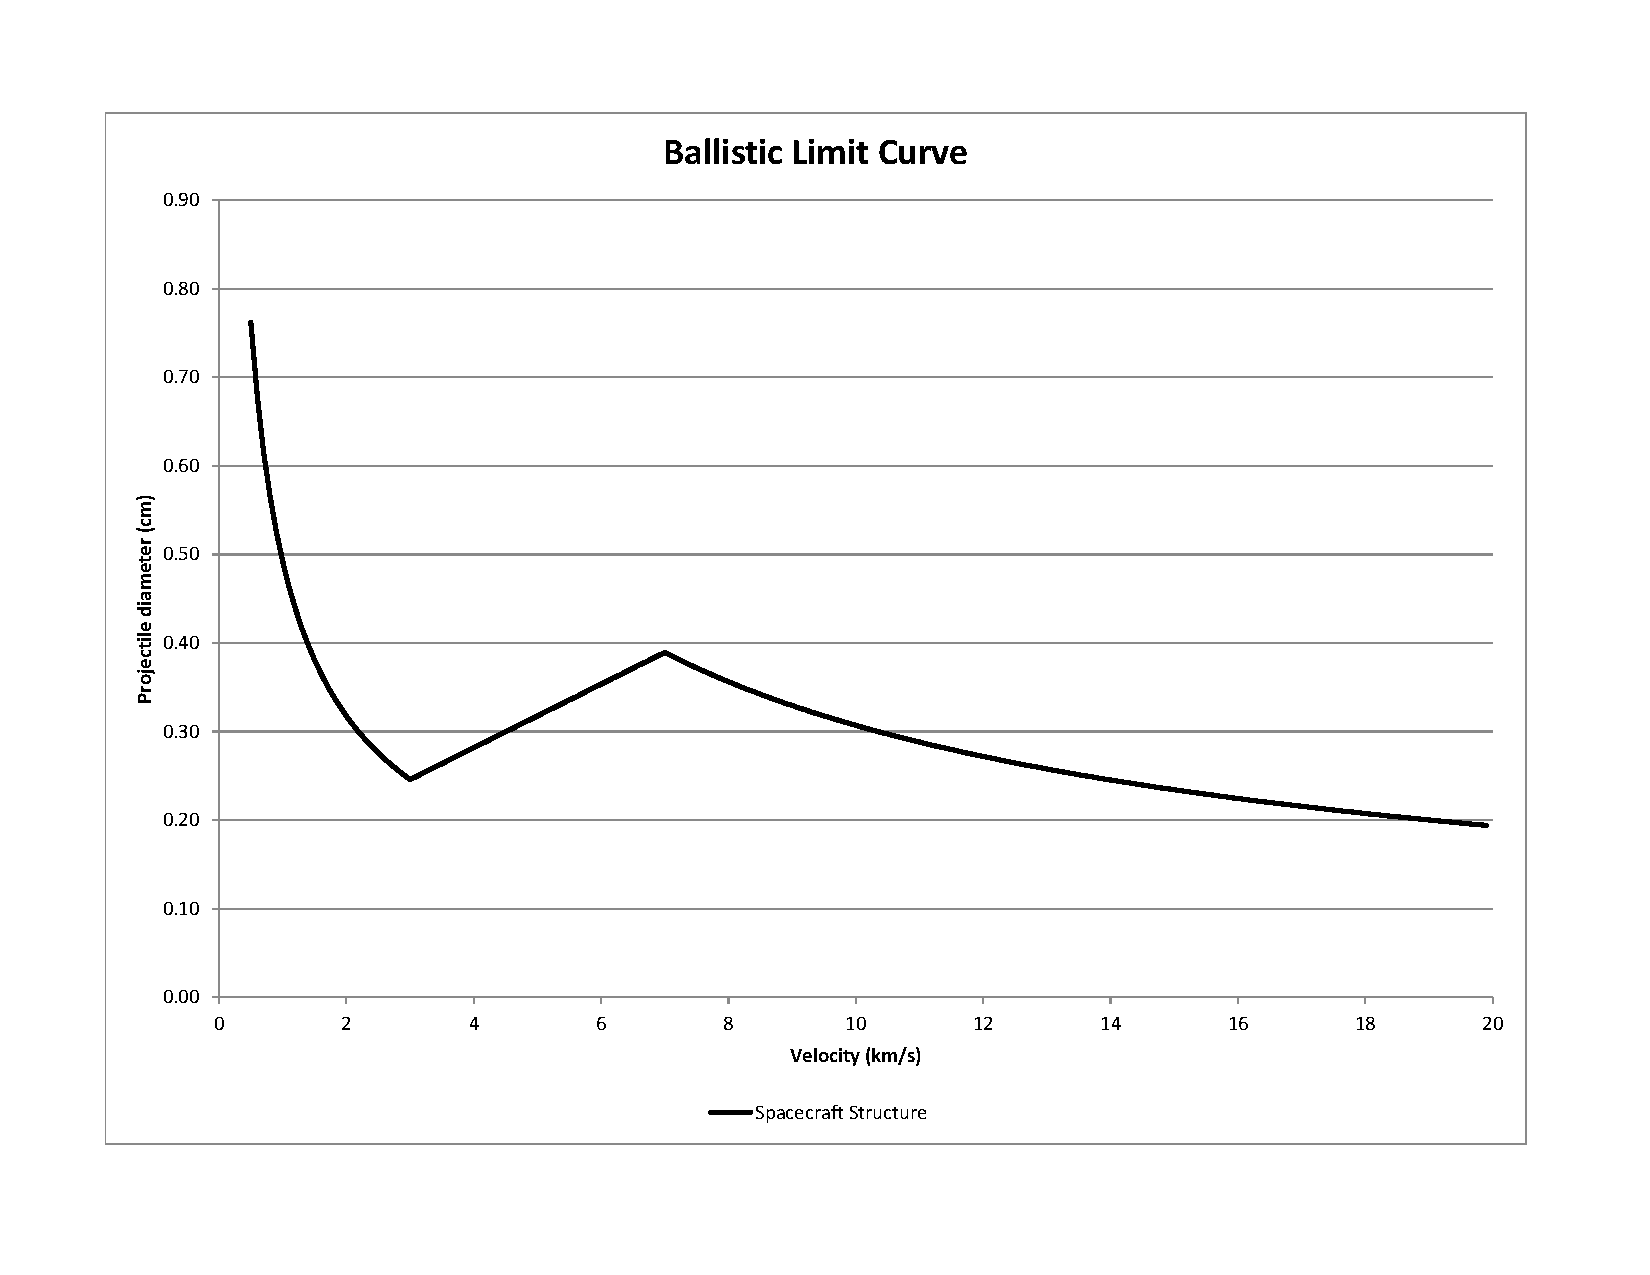
\includegraphics[width=5in]{MMODstructure.pdf}
	\caption{Ballistic limit curve for spacecraft structure.}
	\label{fig:MMODstructure}
	\end{center}
\end{figure}

\subsection{MMOD Ballistic Testing}
With the 3 inch Stuffed whipple shield configuration chosen as the ideal shielding for the spacecraft, now it should undergo testing to ensure that it will live up to the design equations. To test the shielding a simple setup can be made where a small piece of the shielding is help in place while projectiles are shot at it. The projectiles will be shot using a rail gun. The goal is for all projectiles within specified tolerances to not pass through the shielding. Since it's highly unlikely that debris hit the same spot twice it can be shot at either different spots or a different target for each test if the shielding is damaged.

%----------------------------------------------------------------------------------------
%	CONCLUSION
%----------------------------------------------------------------------------------------

\section{Conclusion}

The Hubble Space Telescope has performed and aided great feats of science that have made humans more cognizant of the outside world. The James Webb telescope, although deemed a successor to the HST, will not be able to perform as proficiently in fields that the HST specialized in. It has been recognized that the HST is an irreplaceable article of the scientific community whose loss will affect many fields of research. Therefore, this team of engineers tasked to extend the life of the HST until October 2028.

The stakeholder requirements, as discussed in section 2, have generated further technical and systemic requirements that resulted in comprehensive trade studies across the entire design space. In a systematic fashion, design drivers were identified for each subsystem and decisions were made in a flow-down and iterative manner.

At the onset of the design study, various failure modes were investigated to both protect the HST and to increase assurance in the mission. All identified extreme and high-risk failure modes have been successfully reduced to moderate and low risk statuses. Continual design iteration and testing will expand current FMEA analysis and further aid risk mitigation.

Afterwards, the in-space mission was addressed where the HRV's mass was estimated by methodically studying different rendezvous missions and boosting procedures while considering the Sun's solar cycles and the effect of drag. With the aid of various engineering tools such as AGI's Systems Tool Kit, numerous simulations were conducted in order to ensure HST survival until October 2028. At the end of this study, an appropriate altitude of 616 km was chosen.

The propulsion system was then designed after a structural analysis on the HST solar booms placed an upper limit on thrust output and a rendezvous analysis specified the amount of fuel needed for proximity operations. To protect the HST, cold gas thrusters will be used while a replica of the HST docking mechanism will be attached to the HRV for low risk operations. The sensors required for successful proximity operations have been sized based on the capture limits of the SCM and its convenient targeting system.  After docking, the HST will command attitude adjustments while the HRV boosts it to the final altitude.

To power the spacecraft during the mission, a power budget analysis was performed to pinpoint energy-intensive mission phases. In addition, solar activity and eclipse periods were considered to ultimately size solar panels and batteries for this mission. The disturbances characterizing the space environment, alongside the limited amount of power, directed the design of the attitude and control system. This critical system will ensure mission success during sensitive phases such as rendezvous and orbital transfer while providing crucial information on the HRV's state vector to both the spacecraft and ground control through the TDRSS satellites.

The above subsystems ultimately determine the mass and shape of the HRV bus and, therefore, the launcher used to transport the HRV into space. After a careful trades study, the Delta II launcher was chosen. As a result, the diverse launch environment, which consists of vibro-acoustics, shocks, and intense g-loadings, was used to analyze the structural integrity of the HRV. Using Aluminum 6061-T6, it was found that the HRV will be able to handle the harsh launch environment. Additional precautions were taken, per the requirements, to provide protection against MMODs. In making a compromise between mass and volume, the stuffed whipple shield is projected to protect the spacecraft with 99.99\% probability of no penetration.

The above analysis, stakeholder and technical requirements all birthed a 1080 kg, 1.85 m x 1.85 m x 2.2 m bus that will ride the Delta II rocket to a 200 km circular orbit.  All requirements have been met by this team of engineers so that the total mission, after launch in September 2019 to HRV deorbit, is estimated to run no longer than 60 hours.

% \nocite{*}
\bibliographystyle{IEEETran}
\bibliography{bib}{}

%----------------------------------------------------------------------------------------
%	APPENDIX
%----------------------------------------------------------------------------------------

\newpage
\appendix

% this can also be downloaded with the title (appendix) if getting the appendix title on the correct page is giving you trouble :)
% \includepdf[pages=-, landscape]{lFMEA.pdf}

\includepdf[pages=1, pagecommand=\section{Failure Modes and Effects Analysis} \label{App:FMEA}, scale=0.75, landscape]{AppendixA.pdf}

\includepdf[pages=2, pagecommand=, scale=0.75, landscape]{AppendixA.pdf}

\includepdf[pages=-, pagecommand=\section{Delta V and Mass Calculations}, scale=0.75, landscape]{DeltaVandMass.pdf}

\includepdf[pages=-, pagecommand=\section{Subsystem Mass Breakdown}, scale=0.75,]{SubsystemMass.pdf}

\section{Orbital Decay Script} \label{App:orb}
\lstinputlisting[caption=Orbital decay python script.]{../decay.py}

\section{Historical Data}
% \begin{table}[H]
% \begin{center}
% \begin{tabular}{|c |c |c |c |c|}
% % \toprule
% \hline
% Maneuver & Time, MET & System & $\Delta$V, ft/sec & Duration, sec \\
% % \midrule
% \hline
% NC-1  & 00:05:27:28.9 & OMS (Both) & 98.0 & 59.2 \\ \hline
% NSR   & 01:03:43:59.7 & OMS (Both) & 49.8  & 30 \\ \hline
% NC-2  & 01:04:17:14.3 & OMS (Left) & 14.1 & 17.1 \\ \hline
% NC-3  & 01:17:55:30.1 & OMS (Right) & 12.1 & 14.8 \\ \hline
% % \bottomrule
% \end{tabular}
% \end{center}
% \caption{STS-61. The HST was grappled at 01:23:19:56 and berthed at 01:23:57:30.}
% % \label{properties}
% \end{table}

% % \begin{table}[H]
% % \begin{center}
% % \begin{tabular}{|c |c |c |c |c|}
% % % \toprule
% % \hline
% % Maneuver & Time, MET & System & $\Delta$V, ft/sec & Duration, sec \\
% % % \midrule
% % \hline
% % Reboost 1  & 06:16:59 & RCS Vernier (?) & - & 61 \\ \hline
% % % \bottomrule
% % \end{tabular}
% % \end{center}
% % \caption{STS-61. The HST was grappled at 01:23:28 and berthed at 2:00:10.}
% % % \label{properties}
% % \end{table}

% \begin{table}[H]
% \begin{center}
% \begin{tabular}{|c |c |c |c |c|}
% % \toprule
% \hline
% Maneuver & Time, MET & System & $\Delta$V, ft/sec & Duration, sec \\
% % \midrule
% \hline
% NSR   & 01:03:36:21.9  & OMS         & 96  & 56.2 \\ \hline
% NC-2  & 01:05:02:00    & RCS Primary & 3.1 & 13.0 \\ \hline
% NH    & 01:17:06:04.9  & OMS         & 12  & 8.0  \\ \hline
% NC-3  & 01:17:53:00    & RCS Primary & 3.4 & 14.0 \\ \hline
% NPC-2 & 01:19:00:24    & RCS Primary & 0.5 & 2.0  \\ \hline
% NCC   & 01:20:07:46    & RCS Primary & 1.1 & 1.1  \\ \hline
% TI    & 01:21:07:52    & RCS Primary & 2.8 & 12.0 \\ \hline
% MC-1  & 01:21:34:16    & RCS Primary & 0.4 & 2.0  \\ \hline
% MC-2  & 01:22:02:40    & RCS Primary & 1.5 & 6.0  \\ \hline
% MC-3  & 01:22:12:40    & RCS Primary & 0.9 & 3.0  \\ \hline
% MC-4  & 01:22:22:40    & RCS Vernier & 0.2 & 1.0  \\ \hline
% % \bottomrule
% \end{tabular}
% \end{center}
% \caption{STS-82. The HST was grappled at 01:23:28 and berthed at 2:00:10.}
% % \label{properties}
% \end{table}

% % \begin{table}[H]
% % \begin{center}
% % \begin{tabular}{|c |c |c |c |c|}
% % % \toprule
% % \hline
% % Maneuver & Time, MET & System & $\Delta$V, ft/sec & Duration, min:sec \\
% % % \midrule
% % \hline
% % Reboost 1 & 04:01:09:28 & RCS Vernier & 6.6  & 20:41.9 \\ \hline
% % Reboost 1A$_a$ & 04:06:07:04 & RCS Vernier & 3.3  & 10:12.6 \\ \hline
% % Reboost 2 & 5:01:15:03 & RCS Vernier & 6.5  & 19:46.9 \\ \hline
% % Reboost 3 & 07:01:33:00 & RCS Vernier & 10.4 & 31:53.5 \\ \hline
% % % \bottomrule
% % \end{tabular}
% % \end{center}
% % \caption{STS-82. a - Manuever required for space debris avoidance. The four reboost maneuvers raised the HST orbit an average of 8 nmi.}
% % % \label{properties}
% % \end{table}

\begin{table}[H]
\begin{center}
\begin{tabular}{|c |c |c |c |c|}
% \toprule
\hline
Maneuver & Time, MET & System & $\Delta$V, ft/sec & Duration, sec \\
% \midrule
\hline
NC-1 Trim & 01:03:42:23    & RCS Primary & 0.06 & 0.44   \\ \hline
NC-2      & 01:04:36:49    & RCS Primary & 7.4  & 31     \\ \hline
NSR Trim  & 01:17:36:55.1  & RCS Primary & 0.2  & 0.24   \\ \hline
NCC       & 01:20:38:00    & RCS Primary & 0.3  & 1.0    \\ \hline
TI        & 01:21:36:06    & RCS Primary & 4.1  & 8.7    \\ \hline
MC-1      & 01:21:58:06    & RCS Primary & 0.3  & 0.5    \\ \hline
MC-2      & 01:22:32:58    & RCS Primary & 0.9  & 2.9    \\ \hline
MC-3      & 01:22:49:58    & RCS Primary & 0.4  & 1.0    \\ \hline
MC-4      & 01:22:59:58    & RCS Vernier & 1.8  & 7.2    \\ \hline
% \bottomrule
\end{tabular}
\end{center}
\caption{STS-103. The HST was grappled at 01:23:44:01 and berthed at 2:00:52.}
% \label{properties}
\end{table}


\begin{table}[H]
\begin{center}
\begin{tabular}{|c |c |c |c |c|}
% \toprule
\hline
Maneuver & Time, MET & System & $\Delta$V, ft/sec & Duration, sec \\
% \midrule
\hline
NC2  & 000:17:50:50.5 & -X RCS & 4.5 & 19.7 \\ \hline
NC3  & 01:02:55:32    & Multi-axis RCS & 3.1 & 12.6 \\ \hline
NC4  & 01:17:47:01    & Multi-axis RCS & 4.8 & 20.4 \\ \hline
NCC  & 01:18:38:57    & Multi-axis RCS & 1.3 & 5.5 \\ \hline
MC-1 & 01:19:59:04    & Multi-axis RCS & 0.8 & 3.2 \\ \hline
MC-2 & 01:20:34:27    & Multi-axis RCS & 0.4 & 1.79 \\ \hline
MC-3 & 01:20:34:27    & +X RCS & 1.9 & 8.1 \\ \hline
MC-4 & 01:21:01:28    & Multi-axis RCS & 1.9 & 8.1 \\ \hline
% \bottomrule
\end{tabular}
\end{center}
\caption{STS-109. The HST was captured at 001:21:09:19.}
% \label{properties}
\end{table}

% \begin{table}[H]
% \begin{center}
% \begin{tabular}{|c |c |c |c |c|}
% % \toprule
% \hline
% Maneuver & Time, MET & System & $\Delta$V, ft/sec & Duration, min:sec \\
% % \midrule
% \hline
% Reboost 1 & 07:05:56:01.8 & RCS Vernier (?) & 11.8  & 36:00 \\ \hline
% % \bottomrule
% \end{tabular}
% \end{center}
% \caption{STS-109. The reboost maneuver raised the HST orbit an average of 3.6 nmi.}
% % \label{properties}
% \end{table}

\begin{table}[H]
\begin{center}
\begin{tabular}{|c |c |c |c |c|}
% \toprule
\hline
Maneuver & Time, GMT & System & $\Delta$V, ft/sec & Duration, sec \\
% \midrule
\hline
NC 1 & 131/21:49:54.65 & RCS & 19.5 & 90.88   \\ \hline
NCC  & 133/13:41:50    & RCS &  1.6 & 7.0     \\ \hline
MC 3 & 133/15:53:26.3  & RCS &  0.9 & 0.2     \\ \hline
MC 4 & 133/16:03:26.5  & RCS &  2.1 & 8.9     \\ \hline
% \bottomrule
\end{tabular}
\end{center}
\caption{STS-125. The HST was captured at 133/17:30:52.}
% \label{properties}
\end{table}

%----------------------------------------------------------------------------------------

\end{document}
